\documentclass[headings=standardclasses,headings=big,oneside,a4paper,openany,12pt]{scrbook}

\newcommand {\e}[1]{\mathrm{~#1}}
\newcommand {\E}[1]{\times 10^{#1}}
\newcommand {\vars}{$\Delta E$ and $M_{BC}$}
\newcommand {\btbii}{\texttt{B2BII}}
\newcommand {\decaya}{$B \rightarrow K K \ell \nu$}
\newcommand {\decayb}{$B^+ \rightarrow K^+ K^- \ell^+ \nu$}

%\usepackage{biblatex}
%\bibliography{mybib.bib} 
\usepackage[english]{babel}% Recommended
\usepackage{csquotes}% Recommended
\usepackage[sorting=none,firstinits=true,backend=bibtex]{biblatex}
\addbibresource{mybib.bib}% Syntax for version >= 1.2

\usepackage{paralist}
\usepackage{caption}
\usepackage{cancel}

\usepackage{longtable}

\setlength{\parskip}{1em}%
\setlength{\parindent}{0cm}

\usepackage{titling}
\usepackage{amsmath,amssymb,amsfonts,nicefrac}
\usepackage{graphicx}
\usepackage{color}
\usepackage{float}
\usepackage{mathtools}
\allowdisplaybreaks
\usepackage[pdftex,colorlinks=true,citecolor=blue,linkcolor=black,urlcolor=blue,bookmarks=true]{hyperref}
\usepackage{dictsym}
\usepackage{braket}
\usepackage{slashed}
\DeclareMathOperator{\arcsinh}{arcsinh}
\usepackage{enumerate}
\usepackage{array}
\setlength{\extrarowheight}{.5ex}

\usepackage{lineno}
\linenumbers

\usepackage{subfigure}

\title{{\Large BELLE NOTE 1486}\\\huge {Measurement of the decay $B^+ \to K^+K^-\ell^+\nu_\ell$ with B2BII}}
\author{Matic Lubej}
\date{Ljubljana, 2018}
%
%
\begin{document}
\begin{titlingpage} %This starts the title page
\phantom{test}
\vspace{5cm}

\begin{center}
\thetitle
\vspace{0.5 cm} \\
{\Large \theauthor}\\
\vfill
{\Large\thedate}
\end{center}
\end{titlingpage}

\pagestyle{plain}
\pagenumbering{roman}

\chapter*{Changelog}

\begin{itemize}
\item First submission of the note.
\end{itemize}

\tableofcontents
\addtocontents{toc}{~\hfill\textbf{Page}\par}

\chapter{Introduction}

%TODO: add references
\pagenumbering{arabic}
Particle physics is already an established branch of physics with a rich history in theory and experiments ever since the beginning of the 20th century. So far the experimental and theoretical research have shown us hand in hand that the universe consists of particles and force carriers. Particles of matter, or elementary particles, are divided into two groups, quarks and leptons. The quarks that we know today are called $u$ (up), $d$ (down), $s$ (strange), $c$ (charm), $b$ (bottom) and $t$ (top). Leptons are split into two groups; charged leptons $e$ (electron), $\mu$ (muon), $\tau$ (tau lepton) and corresponding neutrinos $\nu_e$ (electron neutrino), $\nu_\mu$ (muon neutrino), $\nu_\tau$ (tau neutrino). Particles of force are known as gauge bosons and they are $\gamma$ (photon), $g$ (gluons), $W^\pm$ (charged weak bosons) and $Z^0$ (neutral weak boson). The theory also predicted the recently discovered Higgs boson ($H$), which is responsible for the mass of all particles. Some of the particles above also have a mirrored version of themselves, called antiparticles, which exhibit somewhat different properties as their un-mirrored versions.

Combinations of quarks such as $q_1 q_2 q_3$ (hadrons) or $q_1 \bar{q}_2$ (mesons) can make up heavier particles that we see today. Such particles are protons and neutrons, but also heavier particles which can be produced in processes involving very high energies. Such heavy particles are unstable and decay into lighter ones via forces of nature. Together with the elementary particles and force carriers, three out of four of these forces are joined in a theoretical model called the Standard Model (SM), which is shown in Figure \ref{fig:sm}. They are the electromagnetic, weak nuclear and strong nuclear force. Gravity is not included in the current version of the Standard Model due to its nature. By researching such processes in large experiments it is possible to study the mechanism of how elementary particles interact. By doing so we are able to learn secrets of the universe and how it all began.

\begin{figure}[H]
\centering
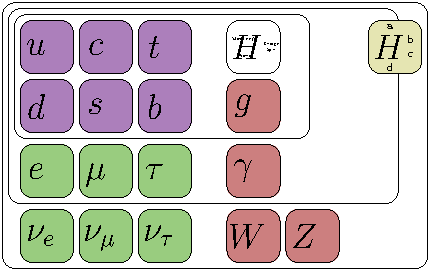
\includegraphics[scale=1.6]{texfig/SM}
\captionsetup{width=.8\linewidth}
\caption{A schematic of the Standard Model.}
\label{fig:sm}
\end{figure}

This analysis revolves around decays of the so called $B$ mesons, which are particles that consist of a $b$ quark and a light $\bar u$ or $\bar d$ quark (or vice-versa). One of the most surprising features of the universe that can be studied with decays of $B$ mesons is the $CP$ symmetry violation ($\cancel{CP}$). $CP$ symmetry is a combination of the $C$ symmetry (charge conjugation) and the $P$ symmetry (spatial inversion). It states that there is no reason why processes of particles and mirrored processes of antiparticles would be different. Today we know that this does not hold for all cases and we in fact find processes which violate this postulate. We also know that $\cancel{CP}$ is very closely related to the the weak nuclear force. Here lies our motivation for studying decays of $B$ mesons, since they exhibit a rich spectrum of decays, many of which underway via the weak nuclear force.

One of the most important properties of the weak nuclear force is that it can change the flavor of particles. Flavor is a quantum number which is conserved for each type of quark, so changing a flavor of a quark means changing the quark itself. Such processes are forbidden for the electromagnetic and the strong nuclear force, but not for the weak one. All of the information regarding quark transitions and transition probabilities can be merged into a form of a complex matrix called the Cabibbo-Kobayashi-Maskawa (CKM) matrix \cite{cabibbo1963unitary,kobayashi1973cp}
\begin{equation}
V_{CKM} = \begin{bmatrix}
    V_{ud} & V_{us} & V_{ub}\\
	V_{cd} & V_{cs} & V_{cb}\\
	V_{td} & V_{ts} & V_{tb}
\end{bmatrix}.
\end{equation}

The CKM matrix is a unitary matrix and has only four free parameters which are not described by theory. Its unitarity provides us with several mathematical identities, out of which the most famous one is
\begin{equation}
V_{ud}V_{ub}^* + V_{cd}V_{cb}^* + V_{td}V_{tb}^* = 0.
\end{equation}

It can be represented by a triangle in the complex plane, called the unitarity triangle, shown in Figure~\ref{ut}. The sides and the angles of the unitarity triangle are closely connected to the free parameters of the CKM matrix. It is important to mention that all experimental measurements depend only on these four parameters, so it is possible to determine them by measuring the angles and sides of the unitarity triangle. This way the unitarity triangle offers us a unique way to test the consistency of the SM. The ultimate goal is to then join all such measurements and overconstrain the unitarity triangle to check if all the sides meet. By improving such measurements one can check whether the SM is consistent, or if there are some contributing physics processes that we do not yet understand. Such processes are commonly referred to as "new physics" (NP). The measurements of the sides and angles of the triangle are done by using different decays of which a large portion are $B$ meson decays. Here lies another motivation for using $B$ mesons in the analysis.

\begin{figure}[H]
\centering
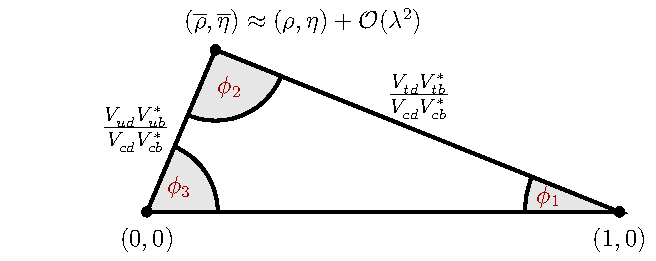
\includegraphics[scale=1]{texfig/UT_Triangle}
\caption{The unitarity triangle with $\lambda,~\eta,~\rho$ and $A$ (not shown) as free parameters of the CKM matrix.}
\label{ut}
\end{figure}

In this analysis we focus on the $V_{ub}$ CKM matrix element, which corresponds to $b \rightarrow u$ quark transitions. It has the smallest absolute value of all the CKM matrix elements and the largest error, so it offers the most room for improvement. Such quark transitions are present in charmless semi-leptonic $B$ meson decays of the form
\begin{equation}
B^+ \to X_u \ell^+ \nu_\ell,
\end{equation}

where $X_u$ represents a charmless hadron with a $u$ quark and $\ell$ one of the charged leptons $e,~\mu$ or $\tau$. Measuring the decay rate of the $B$ meson in such decays offers the way for the CKM matrix element determination. Decay rates are directly connected to the $V_{ub}$ element as
\begin{equation}
\mathrm{d} \Gamma \propto G_F^2 \vert V_{ub} \vert ^2 \vert L^\mu \langle X_u \vert \bar u \gamma_u \frac{1}{2} (1-\gamma_5) b \vert B \rangle \vert ^2,
\end{equation}

where $\Gamma$ is the decay width, $G_F$ is the Fermi coupling constant, $L^\mu$ is the leptonic current and the expression in the Dirac brackets the hadronic current. The factor $\vert V_{ub} \vert ^2$ represents the probability for the $b \rightarrow u$ quark transition. Measurement of the $V_{ub}$ CKM matrix element can be performed in two possible ways. With the exclusive or the inclusive method, which are described below. Both methods require different experimental and theoretical techniques, so they provide largely independent determinations of $V_{ub}$. Currently both methods also have comparable accuracies. %TODO: check if still true

In the exclusive method one studies the decays of $B$ mesons to a specific charmless hadronic final state, such as $B \rightarrow \pi \ell \nu$. Clean determination of the $V_{ub}$ is possible due to precise experimental measurement along with reliable theoretical calculations. However, theoretical calculations are more challenging for decays to a specific final state, since hadronization of quarks has to be taken into account. There are also two main experimental challenges in this method. One has to reduce the much more abundant background from $B \rightarrow X_c \ell \nu$ processes, since the $b \rightarrow c$ quark transition is much more common. The second experimental challenge is to separate the $B$ meson decay with the specific charmless hadronic final state from other $B \rightarrow X_u \ell \nu$ decays, since it roughly populates the same regions of phase-space as the signal decay.

In the inclusive method one studies the decays of $B$ mesons to any charmless hadronic final state $B \to X_u \ell \nu$. In this case, the total decay rate for $b \rightarrow u \ell \nu$ can be calculated accurately, since hadronization does not have to be taken into account. The greater challenge with this method is again the experimental measurement of the total decay rate due to the $B \rightarrow X_c \ell \nu$ background. Experimental sensitivity to $V_{ub}$ is highest where $B \rightarrow X_c \ell \nu$ decays are less dominant. Theory and experiment have to compromise and limit the $V_{ub}$ determination to a region where the signal-to-background ratio is good. Theory takes this into account by reliably calculating the partial decay rate $\Delta \Gamma$, which is more challenging than the total decay rate. One possible and relevant approach to reduce $b \rightarrow c$ background is to reject all events with $K$ particles, or kaons, in the final state. The procedure is also called a $K$-veto. Kaons consist of an $s$ quark, which is mainly produced in $c \rightarrow s$ transitions. This means that if a kaon is found, it is very likely that it originates from a particle with a $c$ quark. 

If $V_{ub}$ is determined with both these methods, the values can be compared. It turns out that consistency between these two results is only marginal, where the difference is at a level of $3\sigma$. In fact, inclusive measurements prefer higher values than exclusive ones. This is known as the $V_{ub}$ puzzle. It is necessary to make further research as to why this difference occurs. The reason could be an unknown experimental or theoretical error, or it is even possible that some NP contributions occur. Part of the reason could be hidden in the selection mentioned before. By performing a $K$-veto, one discards all events with kaons in the final state in order to suppress $b \rightarrow c$ contributions. In this analysis we focus on the charged \decaya~decay, which is very similar to the $B \rightarrow \pi \ell \nu$, except for a production of an $s \bar s$ quark pair, which then combines with final state quarks to form kaons, as shown in Figure~\ref{feynman}. In this case, we have kaons in the final state where the $B$ meson decayed via a $b \rightarrow u$ process. Such decays were discarded in previous $V_{ub}$ determinations with the inclusive method, but in principle they contribute to the result. The results of this analysis should help us make a step closer to solving the $V_{ub}$ puzzle. 

\begin{figure}[H]
\centering
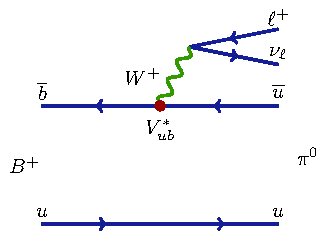
\includegraphics{texfig/B2pilnu}
\hspace{1cm}
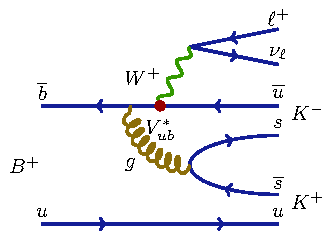
\includegraphics{texfig/B2KKlnu}
\caption{Feynman diagrams for the $B^+ \to \pi^0 \ell^+ \nu_\ell$ decay (left) and the $B^+ \to K^- K^+ \ell^+ \nu_\ell$ decay (right).}
\label{feynman}
\end{figure}

Even though the Belle experiment finished collecting data in 2010, the data is still relevant and available for analysis. On the other hand, Belle II experiment has entered its initial stages of operation. A large part of Belle II software is already available and working, so the practical part of this analysis is done in the framework of the Belle II experiment, called Belle II Analysis Framework (BASF2). The Belle II detector wasn't able to collect a significant amount of data for this analysis, however, the Belle II collaboration developed a data converter for Belle to Belle II format conversion, making it possible to perform analysis of Belle data with Belle II software and enables us to make a relevant contribution despite the transitional period.

Specifically, we will be focusing on decays of the charged $B$ mesons of the form \decayb, since it includes two charged kaons, as opposed to the case of the neutral $B$ meson decay. The reason for this is a simpler decay chain and a higher reconstruction efficiency. All further occurrences of \decaya~automatically imply decays of the form \decayb~and its charge conjugated counterpart.

\chapter{Data and Monte-Carlo samples}\label{sec:data-and-monte-carlo-samples}

The Belle detector acquired a dataset of about $L_0 \approx 710\e{fb^{-1}}$ of integrated luminosity in it's lifetime, which corresponds to about $771\E{6}$ $B \bar B$ meson pairs. Additionally, several streams of Monte-Carlo (MC) samples were produced, where each stream of MC corresponds to the same amount of data that was taken with the detector. The main focus of this and other similar analyses is to study a rare signal decay, which means that the amount of such decays in the existing MC is not abundant enough. In such cases, it is a common practice to produce specific samples of signal MC, where the abundance of signal decays is much larger, enabling us to study it's properties in greater detail.

The following samples were used in this analysis
\begin{itemize}
\item signal MC, corresponding to about $400 \times L_0$,
\item other MC
\begin{itemize}
\item generic, $10$ streams of $B\bar B$ (denoted \texttt{charged} and \texttt{mixed}) and $6$ streams of $q\bar q$ produced at $\Upsilon(4S)$ resonance energy, where each stream corresponds to $L_0$,
\item generic, $6$ streams of $q\bar q$ produced at $60\e{MeV}$ below $\Upsilon(4S)$ resonance energy, where each stream corresponds to $1/10 \times L_0$,
\item $B\to X_u \ell \nu$ (denoted \texttt{ulnu}), not included in previous MC samples, equal to an amount of $20 \times L_0$, 
\item other rare $B$ meson decays (denoted \texttt{rare}), not included in previous MC samples, equal to an amount of $50 \times L_0$, 
\end{itemize}
\item data
\begin{itemize}
\item Belle dataset of about $L_0$ integrated luminosity, measured at $\Upsilon(4S)$ resonance energy,
\item Belle dataset of about $1/10 \times L_0$ integrated luminosity, measured at $60\e{MeV}$ below $\Upsilon(4S)$ resonance energy.
\end{itemize}
\end{itemize}

\section{Signal MC production}

The signal MC sample of $B^+ \to K^+ K^- \ell \nu_\ell$ and the charge conjugated $B^-$ decays was produced using the \texttt{mcproduzh} package for Belle MC generation. The package accepts a decay file, which describes the decays to be generated. The decay file used for signal MC generation was the same as for the $B\to X_u \ell \nu$ generation, since it includes the decays of interest. An additional skim was applied in order to select only events of interest with at least 2 kaons and a light lepton, all coming from the same particle. This decreases the CPU consumption during the detector simulation and reconstruction.

The relevant processes which contribute to our signal decay are
\begin{itemize}
\item $B^+ \to a_{00} \ell^+ \nu_\ell$,
\item $B^+ \to a_{20} \ell^+ \nu_\ell$,
\item $B^+ \to f_{2} \ell^+ \nu_\ell$,
\item $B^+ \to f_{0} \ell^+ \nu_\ell$,
\item $B^+ \to X_{u}^0 \ell^+ \nu_\ell$,
\end{itemize}
where $a_{00}$, $a_{20}$, $f_{2}$ and $f_{0}$ are some of the light unflavored states which in some cases further decay into a $K^+K^-$ pair, while $X_u^0$ represents a generic $u \bar u$ quark pair, which further hadronizes based on the \texttt{PYTHIA} quark hadronization model \cite{sjostrand2006pythia}. %TODO: check this
Figure \ref{fig:KKsrc} shows the invariant mass of the $KK$ pair from various contributions of the MC generator. The light unflavored states have small contributions with resonant structurer, while $KK$ pairs from the $X_u^0$ state are more frequent and follow a wider and smoother distribution.

\begin{figure}[H]
\centering
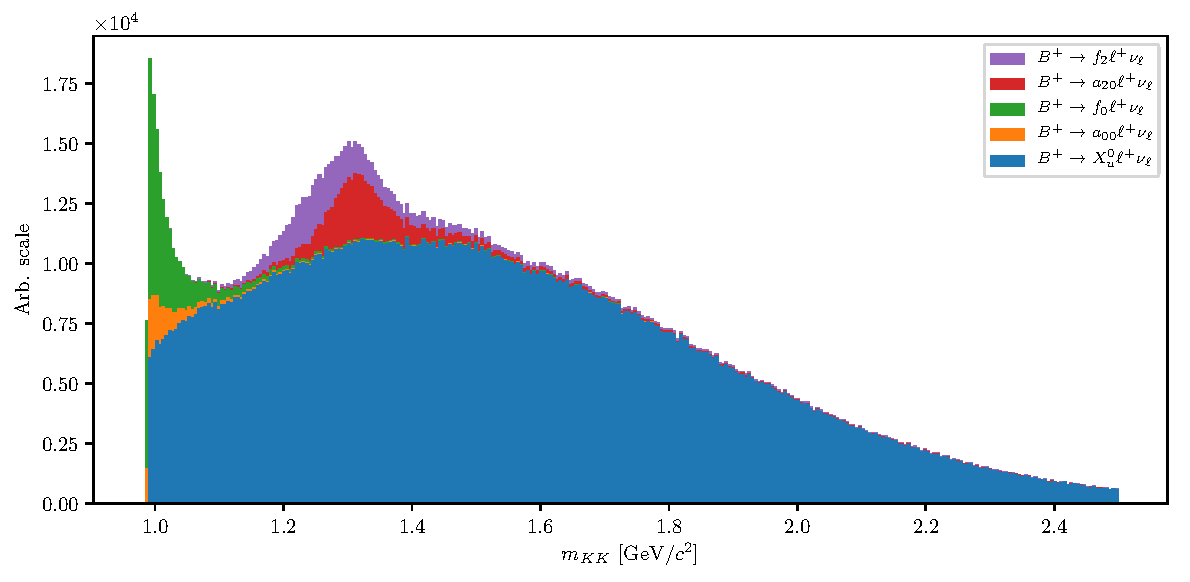
\includegraphics[width=\linewidth]{fig/KKlnu_src}
\captionsetup{width=.8\linewidth}
\caption{Invariant mass of the $KK$ pair from various contributions of the MC generator. The light unflavored states have small contributions with resonant structurer, while $KK$ pairs from the $X_u^0$ state are more frequent and follow a wider and smoother distribution.}
\label{fig:KKsrc}
\end{figure}

The produced signal MC sample contains decays of the form $B \to KK\ell \nu$ as well as $B \to KKX\ell \nu$, where $X$ can be any hadron as long as it satisfies all the selection rules of the decay. It is possible to calculate the MC branching ratios for each channel by making combinations of the particles directly from the generator. Table \ref{tab:KKX} shows some of the most prominent channels, which are similar to our signal decay, as long as their relative fraction. It is clear that our signal decay is the most abundant one, with a relative contribution of about $28.14~\%$, while other channels contribute only up to about $8~\%$ or less. Additionally, our signal decay is also the cleanest, meaning that it has no neutral particles like $\pi^0$, which are harder to reconstruct and suffer from decrease in efficiency due to reconstruction effects.
\begin{table}[H]
\centering
\begin{tabular}{|l|c|}
\hline
Channel & Ratio $[\%]$ \\
\hline 
$K^+ K^-$ & 28.14 \\
\hline
$K^+ K^- \pi^0$ & 8.94 \\
\hline
$K^+ \bar{K}{}^0 \pi^-$ & 8.71 \\
\hline
$K^0 K^- \pi^+$ & 8.70 \\
\hline
$K^+ K^- \pi^+ \pi^-$ & 4.15 \\
\hline
$K^0 \bar K {}^0$ & 3.32 \\
\hline
$K^0 \bar K {}^0 \pi^0$ & 3.26 \\
\hline
$K^+ K^- \rho^0$ & 1.93 \\
\hline
$K^+ \bar{K}{}^0 \rho^-$ & 1.84 \\
\hline
$K^0 K^- \rho^+$ & 1.83 \\
\hline
\end{tabular}
\begin{tabular}{|l|c|}
\hline
Channel & Ratio \\
\hline 
$K^+ K^- \pi^0 \pi^0$ & 0.86 \\
\hline
$K^+ K^- \pi^+ \rho^-$ & 0.69 \\
\hline
$K^+ K^- \rho^+ \pi^-$ & 0.68 \\
\hline
$K^0 \bar K {}^0 \rho^0$ & 0.00 \\
\hline
\hline
$K \bar K$ pair with $\eta$ & 7.08 \\
\hline
$K \bar K$ pair with $\omega$ & 5.33 \\
\hline
Other & 14.53 \\
\hline
\end{tabular}
\caption{Relative branching ratios of $B \to KKX\ell \nu$ decays by channel.}
\label{tab:KKX}
\end{table}

We generate about $1.3\E{9}$ events of the form $B\to X_u \ell \nu$, which corresponds to an integrated luminosity of about $L = 400\times L_0$, where this value was obtained by normalizing the signal MC to the amount of signal in the $B\to X_u \ell \nu$ MC sample. This amounts to a total of about $9.37\E{6}$ generated signal events, and to a branching ratio
\begin{equation}
\mathcal{B}\left(B^+ \to K^+ K^- \ell^+ \nu_\ell\right)_{MC} = 1.53\E{-5},
\end{equation}
where $\ell$ is $e$ or $\mu$. During analysis the abundant signal MC sample is scaled down to correspond to the amount of data taken with the Belle detector.

\chapter{B2BII conversion}

The predecessor of the Belle II experiment was the Belle experiment, which finished its data taking run of 10 years at end of 2010 after collecting a dataset of about $1\e{ab^{-1}}$. That year the Belle detector was shut down and the Belle II experiment was born from the ashes, where even some of the old detector components were reused. The construction of the Belle II detector today is still an ongoing process, although first collisions are expected in 2018. By the year 2025 it is foreseen that Belle II will have recorded about $50\e{ab^{-1}}$ of data, which is about $50$ times more than in case of Belle. However, this is still a long time away, while the recorded dataset of the Belle experiment still has the potential for interesting physics analyses today. On the other hand, most of the people from Belle transitioned to Belle II and a lot of new institutes joined the Belle II Collaboration. This moved focus from Belle analyses and Belle Analysis Framework (BASF) to the construction of the Belle II detector and the development of Belle II Analysis Framework (BASF2), which was written completely from scratch, making the BASF2 software incompatible with the Belle data. This resulted in gradual loss of knowledge on the maintenance and operation of the BASF software.

In the Belle II Collaboration, a task force was created in order to convert Belle data into Belle II format (\btbii). The \btbii~package was developed as a part of BASF2 in order to convert data and MC of the Belle experiment and make it available within BASF2. In addition to the convenience of Belle data being processed in the more intuitive and advanced BASF2 framework, \btbii~allows for estimation and validation of performances of various advanced algorithms being developed for Belle II. The conversion itself, however, is considered non-trivial. Although the conversion of the raw detector data would be possible, the reconstruction algorithms of BASF2 are optimized for Belle II and cannot be effectively applied to Belle data. To bypass this problem, reconstructed objects from \texttt{PANTHER} tables, a custom solution of the Belle collaboration based on C/C++ and Fortran, are mapped to their corresponding representations in BASF2.

The conversion in the \btbii~package is divided into three BASF2 modules. The first module opens the Belle input files and reads the events into memory in the form of \texttt{PANTHER} tables. This module consists predominantly of reused BASF code. The second module applies various calibration factors, such as experiment and run dependent factors, to the beam energy, particle identification information, error matrices of the fitted tracks, etc. The module also applies some low-level cuts to reproduce removing background events as done within BASF. The actual conversion and the mapping of reconstructed objects is done in the last module. For more information see \cite{Keck:48940}.

\section{Validation}

In order to make sure the conversion was successful and without errors, a thorough validation should be performed. This is done by comparing histograms of all physical quantities of the reconstructed objects on simulated and recorded events, processed with BASF and BASF2. Figures X and X show some of the physical properties of the neutral and charged particles, obtained with BASF and BASF2, and their difference. The plots indicate that the conversion is successful and we can proceed with the analysis in the framework of BASF2.

PLOT

PLOT

\chapter{Event reconstruction}

In this chapter the procedure for event reconstruction of the $B$ meson decay $B \to K K \ell \nu$ is shown, starting with final state particle selection and then combining them to obtain $B$ meson candidates.

\section{Final state particles selection}

Since the neutrino escapes detection, we can only reconstruct the charged tracks in the decay, which are the two charged kaons ($K$) and the light lepton, which is the electron ($e$) or muon ($\mu$). These are some of the particles which are commonly referred to as final state particles (FSP). Final state particles have a long lifetime and are usually the particles that we detect when they interact with the material in the detector.

It is important to limit our selection of FSP particles in order to cut down the number of particle combinations,  and consequentially computation time and file sizes.

\subsubsection{Leptons}

Figures \ref{fig:evars} and \ref{fig:muvars} show the impact parameters $d_0$ and $z_0$, the momentum in  $\Upsilon(4S)$ center-of-mass system (CMS), and the PID information for true and fake electrons and muons, where an extra category for true electrons/muons from the signal decay is shown.

\begin{figure}[H]
\centering
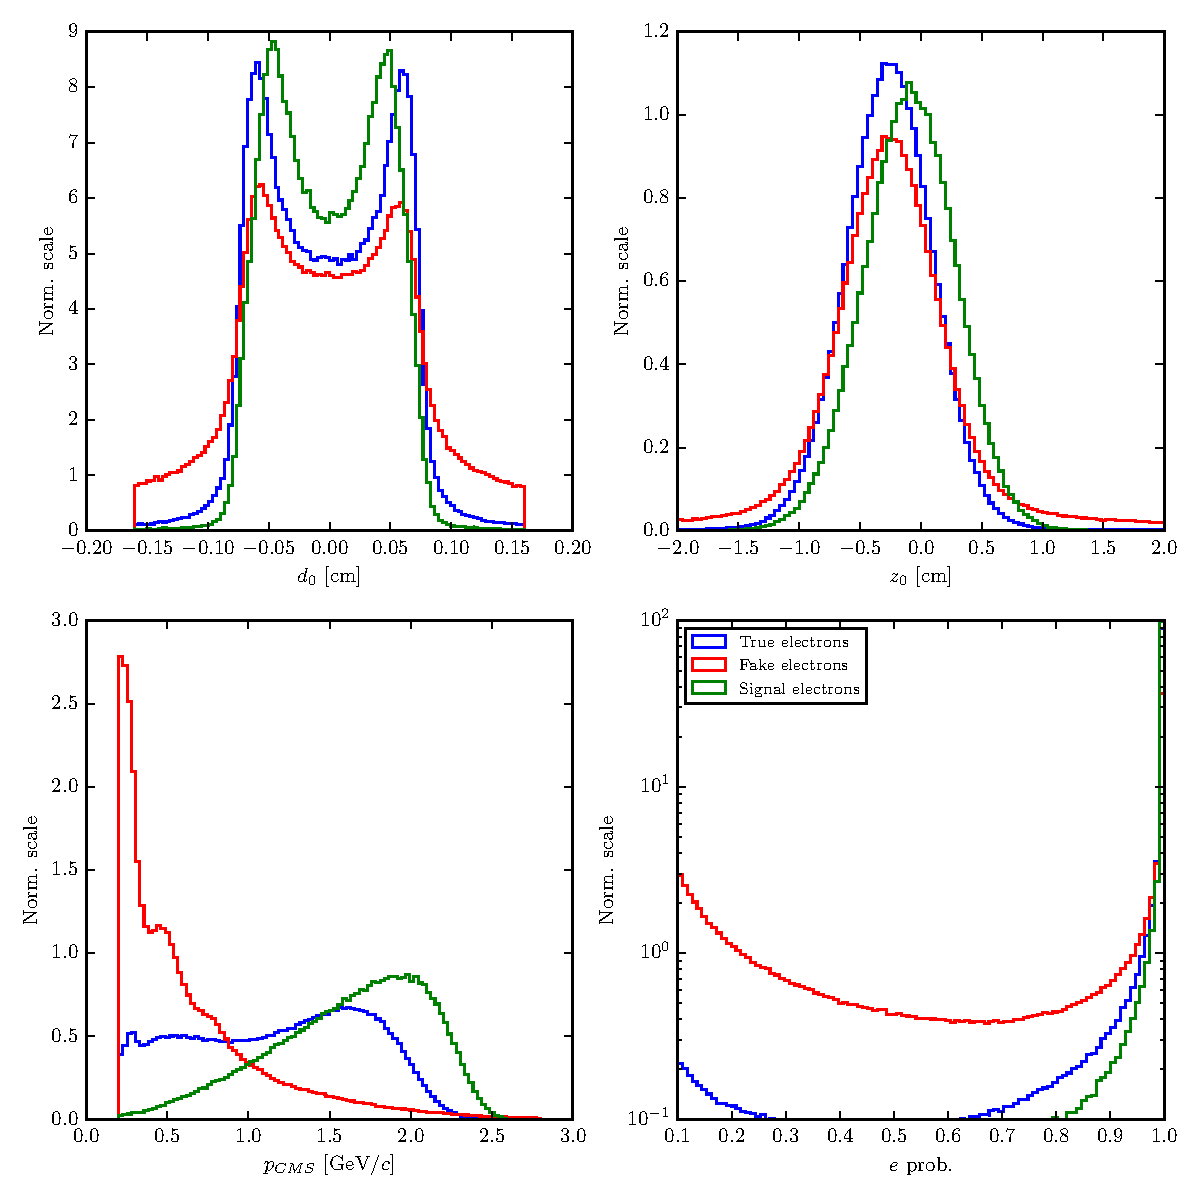
\includegraphics[width=\linewidth]{fig/FSP_e_vars}
\captionsetup{width=.8\linewidth}
\caption{Normalized properties of true (blue), fake (red) and true electrons from signal decay (green).}
\label{fig:evars}
\end{figure}

\begin{figure}[H]
\centering
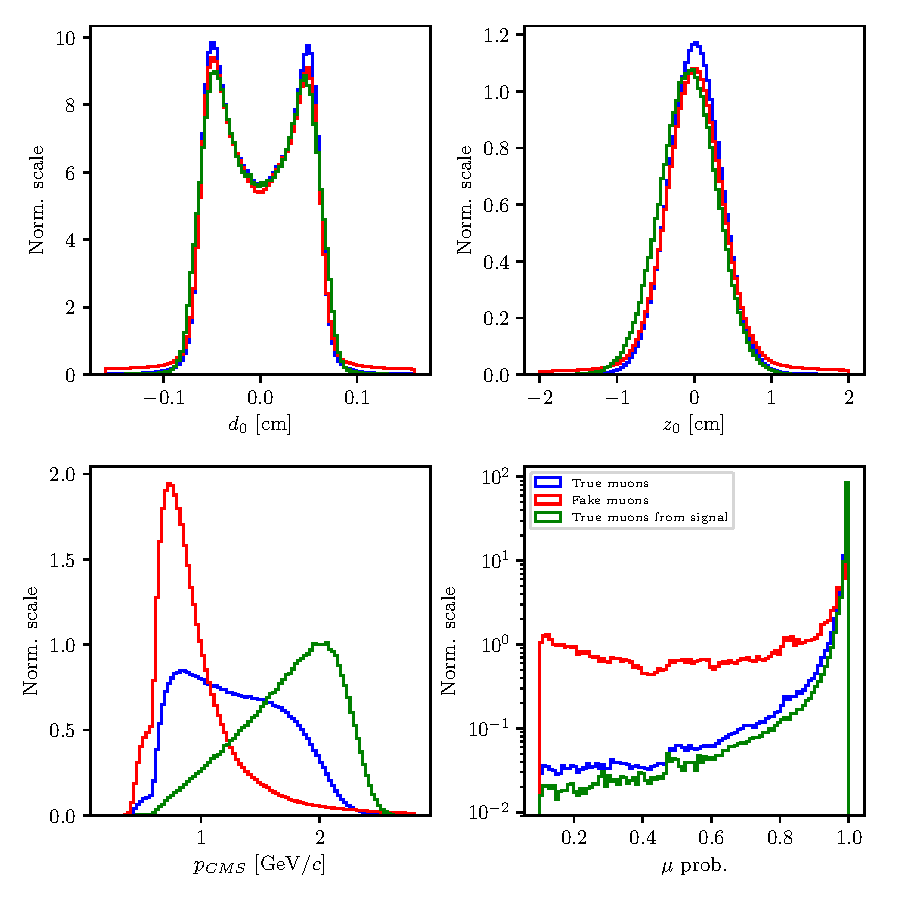
\includegraphics[width=\linewidth]{fig/FSP_mu_vars}
\captionsetup{width=.8\linewidth}
\caption{Normalized properties of true (blue), fake (red) and true muons from signal decay (green).}
\label{fig:muvars}
\end{figure}

Based on these distributions, we can define a set of cuts
\begin{itemize}
\item $\vert d_0 \vert < 0.1\e{cm}$,
\item $\vert z_0 \vert < 1.5\e{cm}$,
\item $p_{CMS} \in [0.4,\,2.6]~\e{GeV}/c$ for electrons,
\item $p_{CMS} \in [0.6,\,2.6]~\e{GeV}/c$ for muons.
\end{itemize}

After this selection we can determine the optimal PID cuts for electrons and muons, where we optimize the selection by maximizing the standard definition of \textit{figure of merit} (FOM), defined in Eq. (\ref{eq:fom})
\begin{equation}
\label{eq:fom}
FOM = \frac{S}{\sqrt{S+B}}.
\end{equation} 
The definition of $S$ and $B$ are somewhat fluid throughout the analysis and need to be defined for each FOM separately. In this section we define two representations of $S$ and $B$. In $FOM_1$ the signal $S$ represents correctly reconstructed particles, while in $FOM_2$ the signal $S$ represents correctly reconstructed particles, which come from a correctly reconstructed $B$ meson candidate. In both cases $B$ represents all other particle candidates which do not satisfy the conditions of $S$.

The $FOM$ plots are shown in Figures \ref{fig:efom} and \ref{fig:mufom}. The cuts values are based on PID cuts used for PID efficiency calibration. The optimal value for the PID cuts is equal to the largest available value, regardless of the leptons coming from signal decays or not. The optimized PID cuts for leptons are
\begin{itemize}
\item $e$ prob. $ > 0.9$ for electrons,
\item $\mu$ prob. $ > 0.97$ for muons.
\end{itemize}

\begin{figure}[H]
\centering
\captionsetup{width=.8\linewidth}
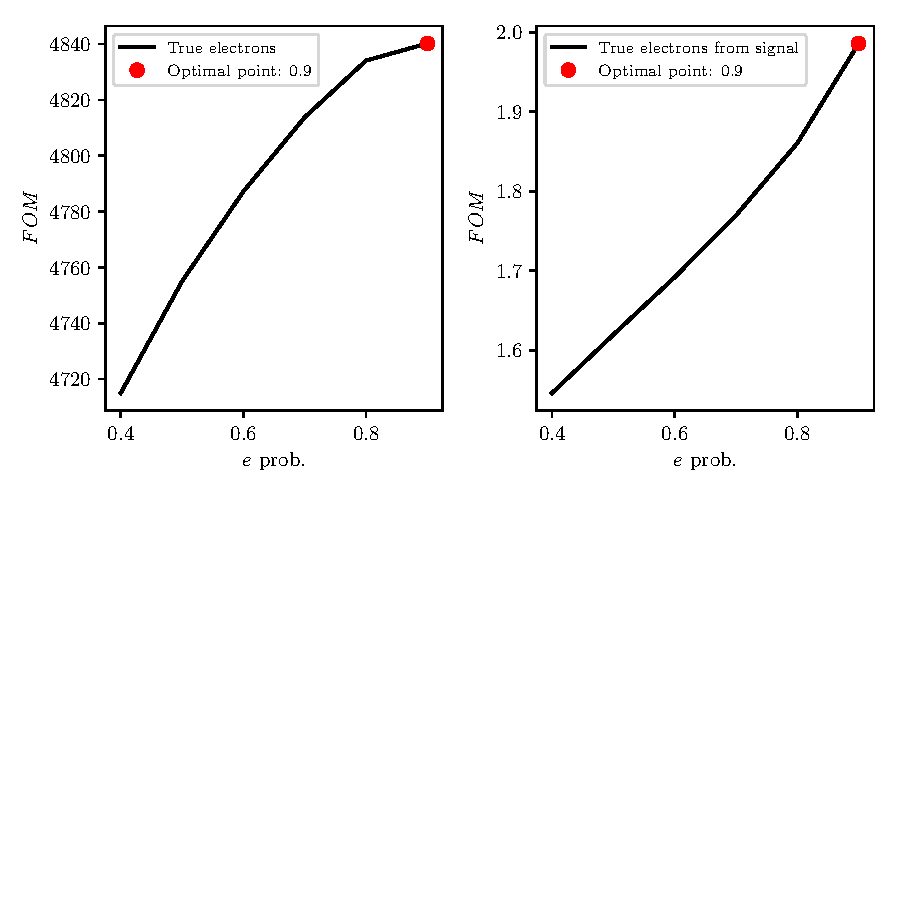
\includegraphics[width=\linewidth]{fig/FSP_e_fom}
\caption{$FOM$ optimizations of the PID probability cuts for true electrons (left) and true electrons from signal decays (right).}
\label{fig:efom}
\end{figure}

\begin{figure}[H]
\centering
\captionsetup{width=.8\linewidth}
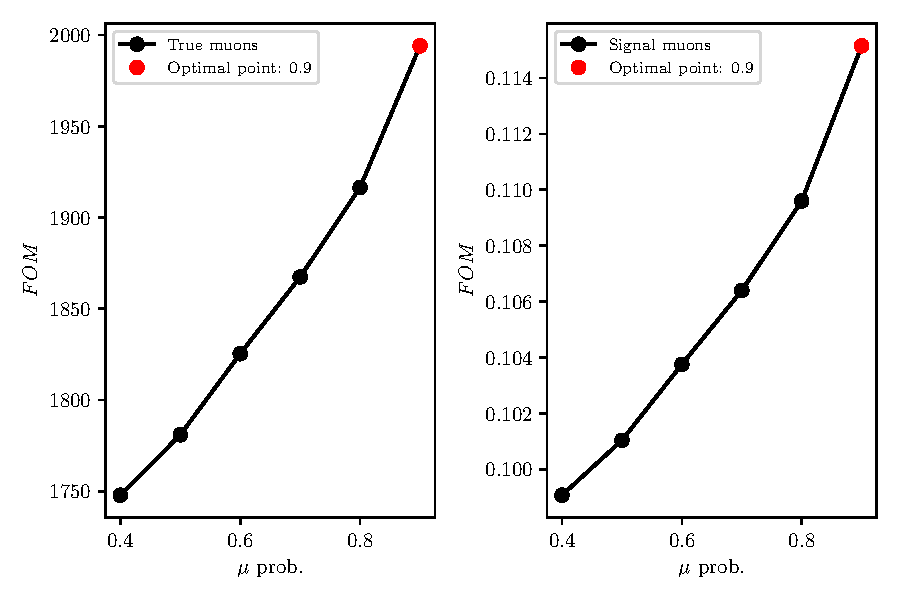
\includegraphics[width=\linewidth]{fig/FSP_mu_fom}
\caption{$FOM$ optimizations of the PID probability cuts for true muons (left) and true muons from signal decays (right).}
\label{fig:mufom}
\end{figure}


\subsubsection{Kaons}

We repeat the procedure for both kaons. Figure \ref{fig:Kvars} shows the impact parameters $d_0$ and $z_0$, the momentum in  $\Upsilon(4S)$ center-of-mass system (CMS), and the PID information for true and fake kaons, where an extra category for true kaons from the signal decay is shown.

\begin{figure}[H]
\centering
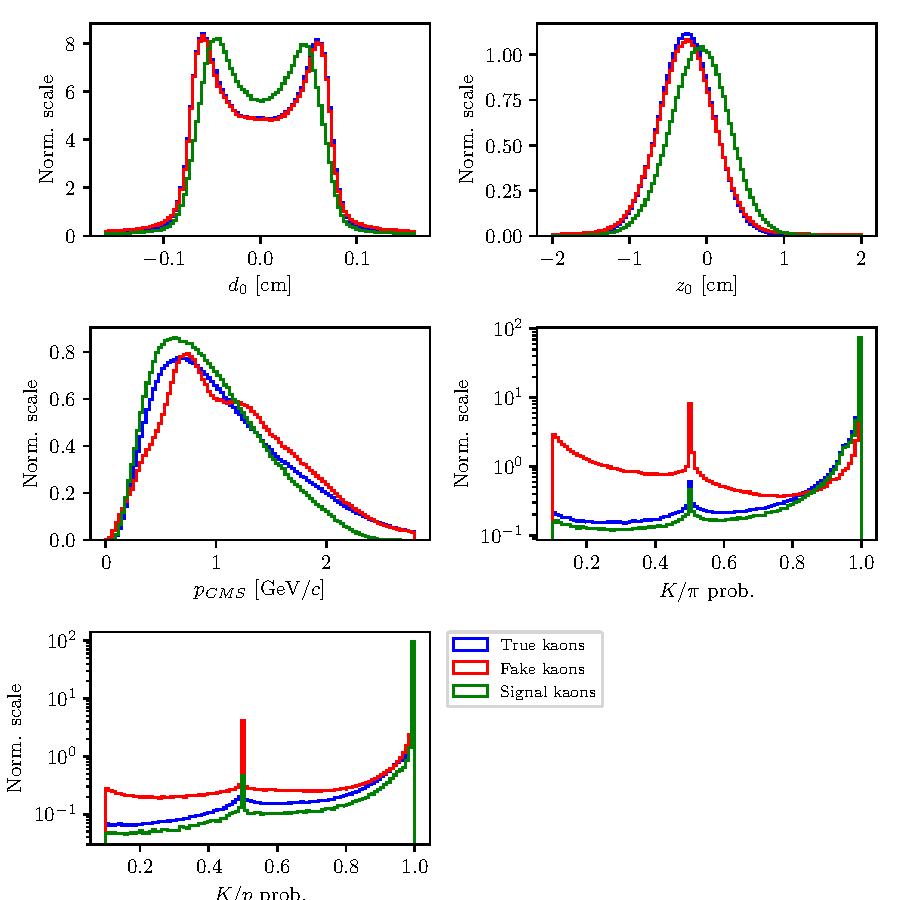
\includegraphics[width=\linewidth]{fig/FSP_kaon_vars}
\captionsetup{width=.8\linewidth}
\caption{Normalized properties of true (blue), fake (red) and true kaons (green) from signal decay.}
\label{fig:Kvars}
\end{figure}

We define the kaon cuts in the same manner as in the case for leptons
\begin{itemize}
\item $\vert d_0 \vert < 0.15\e{cm}$,
\item $\vert z_0 \vert < 1.5\e{cm}$,
\item $p_{CMS} \in [0,\,2.5]~\e{GeV}/c$.
\end{itemize}

The PID optimization in this case is taken in two steps. First we optimize the cut on $K / \pi$, and after that the $K/p$ separation probability. Figure \ref{fig:Kfom} shows the optimization procedure for PID cuts on kaon candidates.

\begin{figure}[H]
\centering
\captionsetup{width=.8\linewidth}
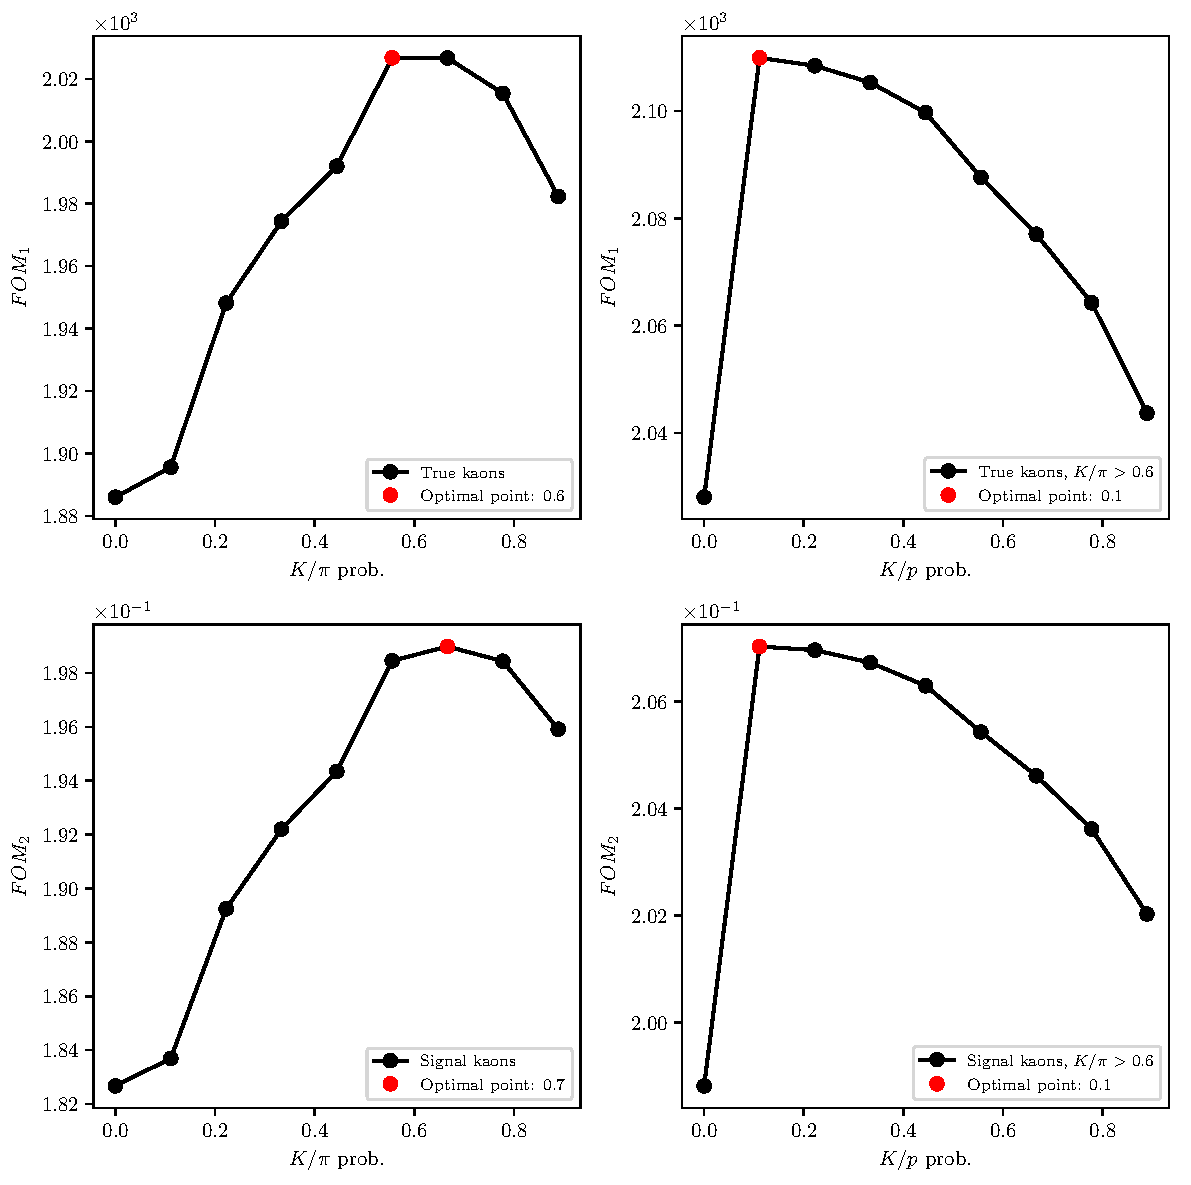
\includegraphics[width=\linewidth]{fig/FSP_kaon_fom}
\caption{$FOM$ optimizations of the PID probability cuts for true kaons (top) and true kaons from signal decays (bottom). The plots on the left show the optimization of the first step for the $K / \pi$ probability cut, and the plot on the right the $K/p$ probability cut.}
\label{fig:Kfom}
\end{figure}

The optimized PID cuts for kaons are
\begin{itemize}
\item $K/\pi > 0.6$,
\item $K/p > 0.1$.
\end{itemize}

\section{Combination of FSP particles}

With the pre-selected kaon and lepton candidates we make combinations for potential $B$ meson candidates. Since the missing neutrino escapes detection, we reconstruct the $B$ mesons in the following two channels
\begin{align*}
B^+ &\to K^+ K^- e^+, \\
B^+ &\to K^+ K^- \mu^+,
\end{align*}
and similarly for $B^-$. When an arbitrary combination is obtained, we perform a vertex fit of the three tracks in order to discard combinations with a low probability of tracks coming from the same point. $B$ mesons have a relatively long lifetime and decay along the z-axis of the detector in the direction of the boost, so the vertex fit is enforced with an \texttt{iptube} constraint, which constrains the vertex to an elongated ellipsoid along beam direction. We demand that the fit converged and apply a cut on the minimal fit probability. The fit probability for signal and background $B$ meson candidates is shown in Figure \ref{fig:vtx} (left). We perform a $FOM$ cut optimization of this variable, which is shown in Figure \ref{fig:vtx} (right). In this and in the following cases, the definition of $S$ from Eq. (\ref{eq:fom}) are correctly reconstructed $B$ meson candidates with a missing neutrino, with an additional constraint that the $B$ meson did not decay via a $b \to c$ transition.

\begin{figure}[H]
\centering
\captionsetup{width=0.8\linewidth}
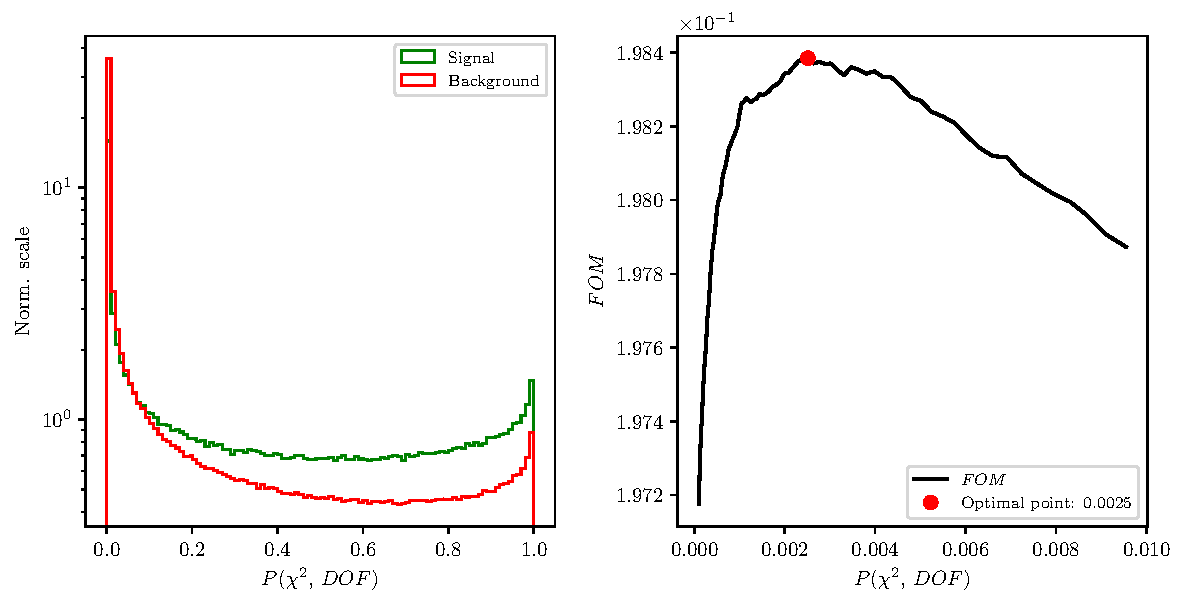
\includegraphics[width=\linewidth]{fig/VTX}
\caption{Normalized vertex fit probability distribution for signal and background $B$ meson candidates in logarithmic scale (left) and $FOM$ optimization of the vertex fit probability (right).}
\label{fig:vtx}
\end{figure}

Even though that the vertex fit probability cut was optimized here, we choose a standard cut of
\begin{itemize}
\item $P(\chi^2,NDF) > 1.0\E{-3}$.
\end{itemize}

With the neutrino being the only missing particle on the reconstructed side, it is possible to determine the angle between the direction of the reconstructed $B$ (denoted as $Y \to K K \ell$) and the true $B$, as
\begin{align}
\mathrm{p}_\nu &= \mathrm{p}_B - \mathrm{p}_{Y}, \\
\label{eq:massnu}
\mathrm{p}_\nu^2 = m_\nu^2 &= m_B^2 + m_Y^2 - 2E_BE_Y + 2\vec{p}_B \cdot \vec{p}_Y \approx 0, \\ 
\label{eq:cosby}
\cos \left(\theta_{BY}\right) &= \frac{2E_BE_Y - m_B^2 - m_Y^2}{2\vert \vec{p}_B \vert \vert \vec{p}_Y\vert},
\end{align} 

where all the energy and momenta above are calculated in the CMS frame. The mass of the neutrino is equal to 0 to a very good precision, so we use it in Eq. (\ref{eq:massnu}). In addition, we can substitute the unknown energy and momentum magnitude, $E_B$ and $\vert \vec{p}_B \vert$, of the $B$ meson in Eq. (\ref{eq:cosby}), with quantities from the well known initial conditions
\begin{align}
E_B &= E_{CMS} / 2,\\
\vert \vec{p}_B \vert = p_B &= \sqrt{E_B^2 - m_B^2},
\end{align} 

where $E_{CMS}$ is the total energy of the $e^+e^-$ collision in the CMS frame and $m_B$ is the nominal mass of the $B$ meson. 

For the correctly reconstructed candidates, this variable lies in the $[-1,1]$ region, though only to a certain precision, due to the finite detector resolution. For background candidates, however, the values populate also the non-physical regions, as is shown in Figure \ref{fig:cosby} (left). We impose an optimized cut on this variable from Figure \ref{fig:cosby} (right) to discard a large amount of background.
\begin{itemize}
\item $\vert \cos \left(\theta_{BY}\right) \vert < 1.0$.
\end{itemize}

\begin{figure}[H]
\centering
\captionsetup{width=.8\linewidth}
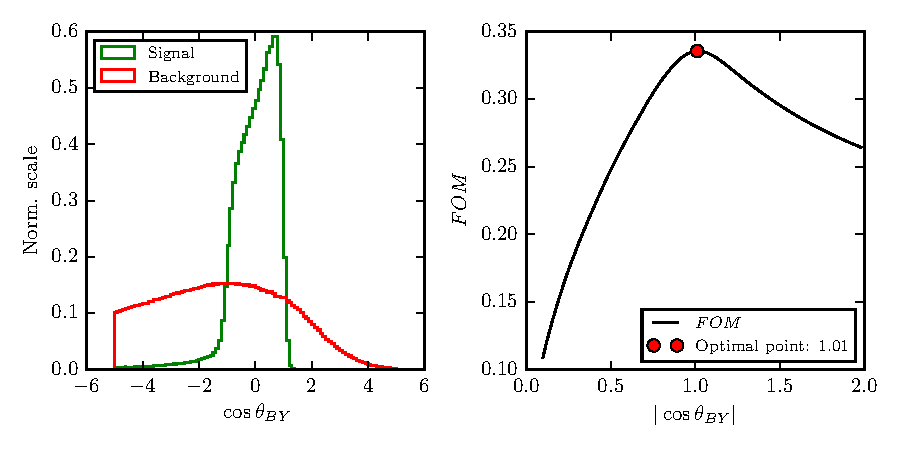
\includegraphics[width=\linewidth]{fig/cosBY}
\caption{Normalized $\cos \theta_{BY}$ distribution for signal and background $B$ meson candidates (left) and $FOM$ optimization of the $\cos \theta_{BY}$ variable (right).}
\label{fig:cosby}
\end{figure}

\section{Loose neutrino reconstruction}\label{sec:loose-neutrino-reconstruction}

%Due to the beam background in the detector, material interactions, or other processes, random tracks and clusters enter our event and get reconstructed as part of the physics process we want to study. These tracks and clusters are not interesting and further spoil the data we measure. In order to remedy this, we perform an extensive clean-up of the tracks and clusters in the ROE side before calculating the four-momentum of the missing part of the event. The clean-up procedure is performed separately on tracks and clusters and uses multiple steps with multivariate analysis (MVA) algorithms in order to separate good tracks and clusters from the bad ones, which populate the ROE. Then, for each ROE object, a ROE mask is created for tracks and clusters, which narrates the use of this track or cluster in the final calculations of the ROE four-momentum.
%
%In order to preserve the continuity of this chapter, a more detailed description of the ROE clean-up can be found in Chapter \ref{ch:roe}. From this point on we assume the ROE to be efficiently cleansed of extra tracks and clusters .


The signal-side neutrino escapes detection, so we cannot directly determine it's four-momentum. However, due to the detectors geometry, which almost completely covers the full solid angle, and due to well known initial conditions of the $\Upsilon(4S)$ meson, it is possible to determine the kinematics of the missing neutrino via indirectly reconstructing the companion $B$ meson by summing up the four-momenta of all the FSP particles in the event which were not used in the reconstruction of the signal side $B$ meson. This is known as the \textit{untagged} method since we are not using any kind of tagging method to reconstruct the companion $B$ meson. The particles used in the indirect companion $B$ meson reconstruction are also said to belong to the \textit{rest of the event} (ROE).

Due to the beam background in the detector, material interactions, or other processes, random tracks and clusters enter our event and get reconstructed as part of the physics process we want to study. These tracks and clusters are not interesting and further spoil the data we measure. In order to remedy this, we perform an extensive clean-up of the tracks and clusters in the ROE side before calculating the four-momentum of the missing part of the event. Here we see the motivation for the ROE clean-up, since our signal candidate reconstruction depends on tracks and clusters in the ROE side. The clean-up procedure is performed separately on tracks and clusters and uses multiple steps with multivariate analysis (MVA) algorithms in order to separate good tracks and clusters from the bad ones, which populate the ROE. Then, for each ROE object, a ROE mask is created for tracks and clusters, which narrates the use of this object in the final calculations of the ROE four-momentum. From this point on we assume the ROE to be efficiently cleansed of extra tracks and clusters. A more detailed description of the ROE clean-up can be found in Chapter \ref{ch:roe}. 

The total missing four-momentum in the event can be determined as
\begin{align}
\mathrm{p}_{miss} &= \mathrm{p}_{\Upsilon(4S)} - \sum_i^{\mathrm{Event}}\left(E_i,\,\vec{p}_i \right),\\
\label{eq:ROEloop}
\mathrm{p}_{miss} &= \mathrm{p}_{\Upsilon(4S)} - \left(\mathrm{p}_{Y} -\sum_i^{\mathrm{Rest~of~event}}\left(E_i,\,\vec{p}_i \right)\right),
\end{align}

where the summation runs over all charged and neutral particles in the defined set with
\begin{equation}
\mathrm{p}^{neutral}_i = \left(p_i,\, \vec{p}_i \right) \quad \mathrm{and} \quad \mathrm{p}^{charged}_i = \left(\sqrt{m_i^2 + p_i^2},\, \vec{p}_i \right),
\label{eq:pcharged}
\end{equation}
where we assumed all neutral particles to be massless photons. For charged tracks in the ROE a mass hypothesis needs to be defined in order to determine the track's energy. After the ROE clean-up we make the following procedure of choosing the mass hypothesis
\begin{enumerate}
\item $e$, if $e$ prob. $> \mu$ prob. and $e$ prob. $> 0.9$,
\item otherwise $\mu$, if $\mu$ prob. $> e$ prob. and $\mu$ prob. $> 0.97$,
\item otherwise $K$, if $K/\pi$ prob. $> 0.6$,
\item otherwise $\pi$.
\end{enumerate} 
We define the square of the missing mass, $m_{miss}^2$, which is zero, if signal-side neutrino is the only missing particle in the event, as shown in Eq. (\ref{eq:m2def}).
\begin{align}
\label{eq:nuold}
\mathrm{p}_\nu &= \mathrm{p}_{miss} = \left(E_{miss},\,\vec{p}_{miss} \right),\\
\label{eq:m2def}
m_{miss}^2 &= \mathrm{p}_{miss}^2 = \mathrm{p}_{\nu}^2 = m_\nu^2 \approx 0.
\end{align}

Since the detector is not perfect, the distribution of the $m_{miss}^2$ variable has a non-zero width. Additionally, tails are introduced as soon as we have missing particles such as extra missing neutrinos, other neutral undetected particles such as $K_L^0$, or simply missing tracks due to detection failure. Figure \ref{fig:missm2} shows the distribution of $m_{miss}^2$ as defined with the missing four-momentum in Eq. (\ref{eq:nuold}). Correctly reconstructed candidates, which come from events where the other $B$ meson decayed via a hadronic decay mode, should peak at zero. If this is not the case, candidates are shifted to larger values of this variable. Due to this fact, we impose a cut on the $m_{miss}^2$ variable in order to partially discard candidates with spoiled properties, even if it was in principle a correct combination of FSP particles on the signal side
\begin{itemize}
\item $\vert m_{miss}^2 \vert < 7\e{GeV}/c^2$.
\end{itemize}
This cut was not optimized, since the optimal case would result in a too strong threshold at this point in the analysis, since we still may want to retain as much signal candidates as possible, even if they are coming from events with semi-leptonic decays of the other $B$ meson.

For further purposes in this analysis we also define a subset of all signal candidates, which come from events where the companion $B$ meson decayed hadronically and all of it's particles were taken into account correctly. We only allow for missing photons, since they are frequently irradiated due to brehmsstrahlung effects and don't have such a big impact on the 4-momentum of the final candidate. We denote this subset as \textit{perfect} signal.

\begin{figure}[H]
\centering
\captionsetup{width=.8\linewidth}
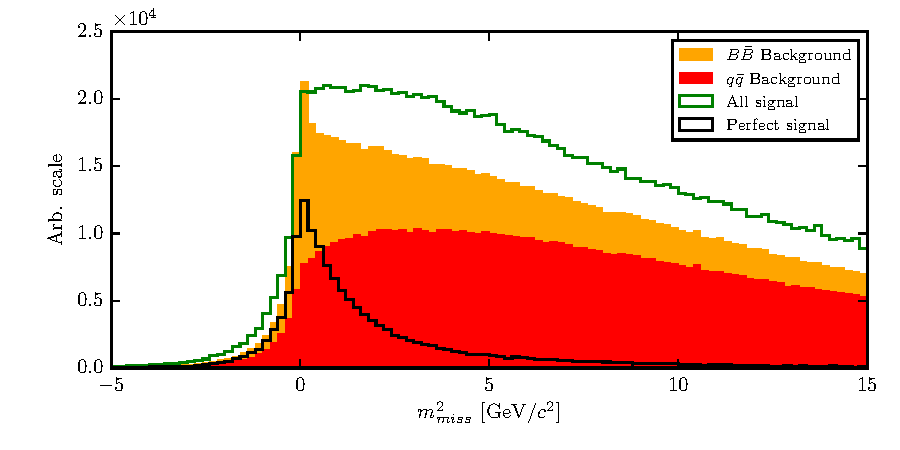
\includegraphics[width=\linewidth]{fig/missM2}
\caption{Squared missing mass distribution for $q \bar q$ and $B \bar B$ background in filled histograms. All signal (green) and perfect signal (black) are scaled up equally.}
\label{fig:missm2}
\end{figure}

The main uncertainty in neutrino four-momentum, defined as in Eq. (\ref{eq:nuold}) comes from energy uncertainty. It is a common practice to substitute the missing energy with the magnitude of the missing momentum, since the momentum resolution from the measurement is much better, thus redefining the neutrino four-momentum to
\begin{equation}
\label{eq:nunew}
\mathrm{p}_\nu = \left(\vert \vec{p}_{miss} \vert,\,\vec{p}_{miss} \right),
\end{equation}
which fixes the neutrino mass to $0\e{GeV}/c^2$.

The newly defined neutrino four-momentum can be added to the four-momentum of the $Y(KK\ell)$ candidate to obtain the full $B$ meson four-momentum and calculate the traditional $M_{BC}$ and $\Delta E$ variables
\begin{align}
\label{eq:de}
\Delta E &= E_B - E_{CMS}/2,\\
M_{BC} &= \sqrt{\left(E_{CMS}/2\right)^2 - \vert \vec{p} \vert^2}.
\end{align}

Since the final fit will be performed over \vars, we define the fit region
\begin{itemize}
\item $M_{BC} \in [5.1,\,5.295]\e{GeV}/c^2$,
\item $\Delta E \in [-1.0,\,1.3]\e{GeV}$.
%\item Signal enhanced region: $M_{BC} \in [5.27,\,5.295]\e{GeV}/c^2$ and $\vert \Delta E \vert < 0.143 \e{GeV}$,
\end{itemize}

Figure \ref{fig:mbc_de_pre} shows the distributions of $\Delta E$ (left) and $M_{BC}$ (right) for signal and major types of background after the pre-cuts. Both signal components are scaled up with respect to the background components, but are in proper scale one to another. The effects of missing particles are clearly seen based on the shape difference between all and perfect signal.

\begin{figure}[H]
\centering
\captionsetup{width=0.8\linewidth}
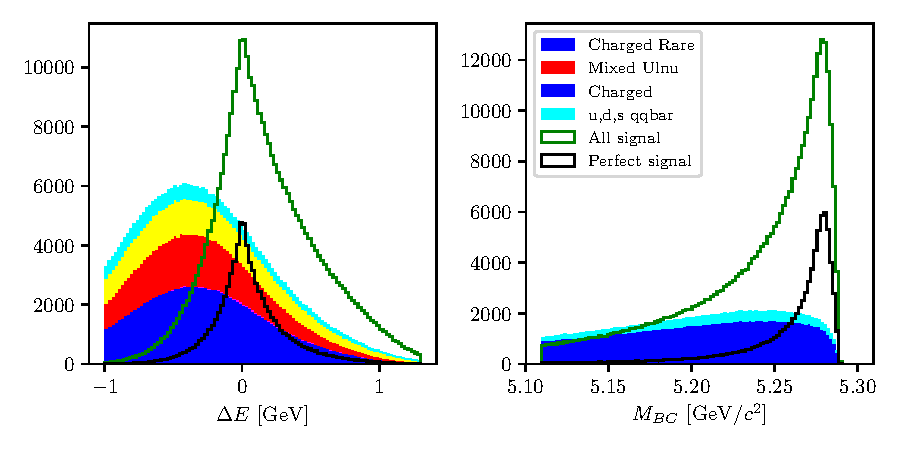
\includegraphics[width=\linewidth]{fig/mbc_de_pre}
\caption{Distributions of $\Delta E$ (left) and $M_{BC}$ (right) for signal and major types of background after the precuts. Both signal components are scaled up with respect to the background components, but are in proper scale one to another. The perfect signal has a much better resolution in both distributions, since the event is perfectly reconstructed.}
\label{fig:mbc_de_pre}
\end{figure}


%\section{$q^2$ calculation}
%
%Momentum transfer squared, $q^2$, is the squared Lorentz invariant of the four-momentum which is transferred from the $B$ meson to the $W$ boson. There are several possible calculations of this variable which offer different resolution. The following describes the calculation of $q^2$ which follows the calculation from [] and yields the best resolution.
%
%For correctly reconstructed events Eq. (\ref{eq:de}) satisfies the condition $\Delta E \approx 0$ within precision. It is possible to rescale the neutrino energy in such way that we fix $\Delta E$ to zero, meaning 
%\begin{equation}
%\Delta E' = (E_Y + \alpha E_\nu) - E_{CMS}/2 = 0.
%\end{equation}
%and calculate and adapted version of $M_{BC}$
%\begin{equation}
%M_{BC}' = \sqrt{\left(E_{CMS}/2\right)^2 - \vert \vec{p}_Y + \alpha \vec{p}_\nu \vert^2}.
%\end{equation}
%
%The neutrino momentum resolution dominates the $\Delta E$ uncertainty [], so the correction factor $\alpha$ reduces this source of uncertainty.
%
%A second correction can be applied by rotating the direction of the neutrino momentum by a small angle with respect to the reconstructed one. Such an angle is chosen in order fix the value of $M_{BC}'$ to the nominal mass of the $B$ meson, $m_B$.
%
%The corrected neutrino momentum is then solely used for the $q^2$ calculation, alongside the reconstructed lepton four-momentum, as
%\begin{equation}
%\label{eq:q2}
%q^2 = \mathrm{q}^2 = \left(\mathrm{p}_\ell + \mathrm{p}_\nu \right)^2.
%\end{equation}
%
%The $q^2$ distribution and its resolution are shown in Figure \ref{fig:q2}, along with additional versions of $q^2$, with details of the calculation method in the caption.
%\begin{figure}[H]
%\centering
%\captionsetup{width=0.8\linewidth}
%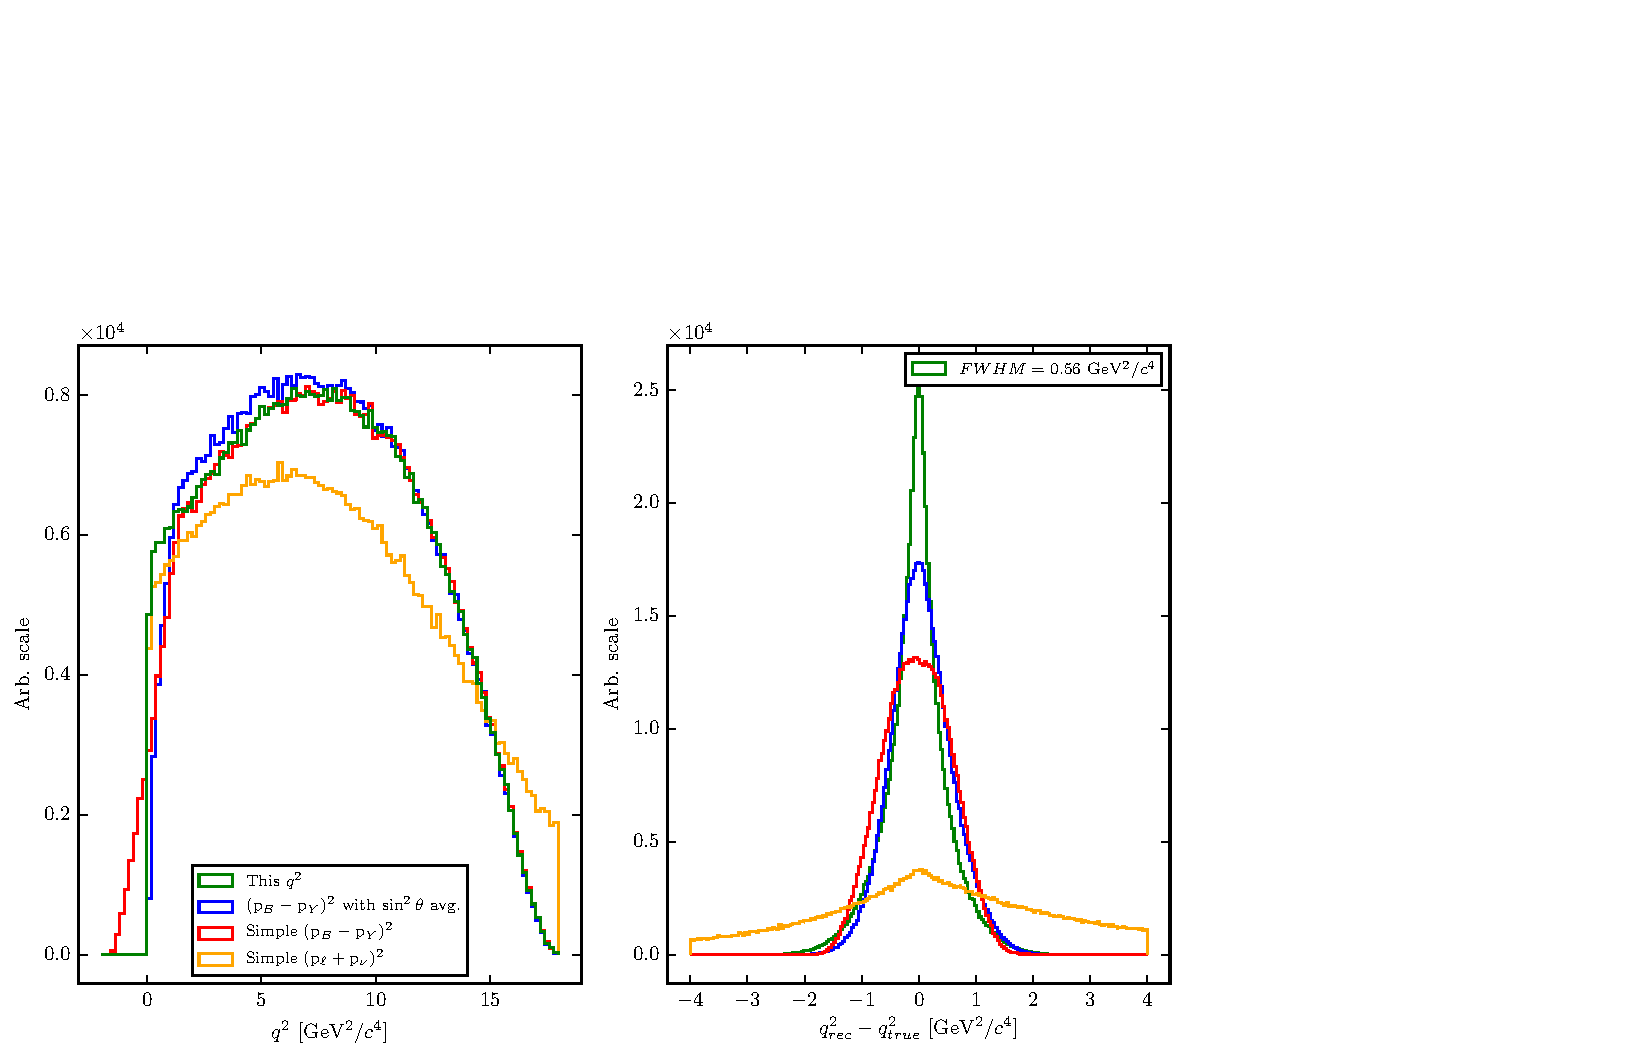
\includegraphics[width=\linewidth]{fig/q2}
%\caption{Distributions of $q^2$ (left) and $q^2$ resolution (right) for various methods of $q^2$ calculation. The blue distribution follows the procedure in [], whereas the red and the orange ones are straight-forward calculations with available information in the reconstruction. The $q^2$ calculation in red assumes a resting $B$ meson in the CMS frame, and the calculation in orange uses the neutrino four-momentum from Eq. (\ref{eq:nuold}).}
%\label{fig:q2}
%\end{figure}
%
%One must bare in mind that even though this calculation yields a precise result, this says nothing about the correctness of the $q^2$ model which was used (ISGW2) []. Since this decay has not been observed yet, we do not have a good description of the decay model, which is also a source of systematics in this analysis.

\section{Event categorization}\label{sec:event-categorization}

The missing information due to an escaping neutrino in our reconstructed channel is replaced by information from the companion $B$ meson. Since this is an untagged reconstruction, the quality of the companion $B$ meson affects the properties of signal candidate. Perfect reconstruction of a hadronically decaying companion $B$ meson results in pronounced peaks at $\Delta E \approx 0$, $m_{miss}^2 \approx 0$ and $M_{BC} \approx m_B$, while imperfect reconstruction due to any kind of missing particles produces long tails and/or a shift from the desired value in the mentioned distributions. These effects are undesired, since they make it harder to separate signal from background.

To remedy this, we split our signal candidates into 4 categories and work only with the best category. For categorization we use splitting in two ways. First, we look at the charge product of the reconstructed $B$ meson and the ROE object. For correctly reconstructed events, this should have a value of 
\begin{equation}
\label{eq:chargeprod}
q_{B_{sig}}~q_{B_{comp}} = -1,
\end{equation}

however, this value is distributed due to missing charged particles in the reconstruction. Secondly, we train an MVA classifier based on ROE object properties in order to recognize companion $B$ mesons, which decayed hadronically. The details of the training are described in subsection \ref{subs:HDMVA}.

We define the 4 categories in the following way
\begin{enumerate} 
\item[]category I: $q_{B^\pm}~q_{B^\mp} = -1$ and $BDT_{had.} > 0.57$,
\item[]category II: $q_{B^\pm}~q_{B^\mp} \neq -1$ and $BDT_{had.} > 0.57$,
\item[]category III: $q_{B^\pm}~q_{B^\mp} = -1$ and $BDT_{had.} \leq 0.57$,
\item[]category IV: $q_{B^\pm}~q_{B^\mp} \neq -1$ and $BDT_{had.} \leq 0.57$,
\end{enumerate}

with the relative ratios of $37.74~\%$, $40.50~\%$, $13.43~\%$ and $8.32~\%$ for categories I, II, III and IV, respectively. Different categories for all signal candidates after the pre-cuts are shown in Figure \ref{fig:sig_categ}. Category I and II represent the majority of the candidates more or less equally, but category I has the best resolution, so we focus on candidates from category I in this analysis.

\begin{figure}[H]
\centering
\captionsetup{width=0.8\linewidth}
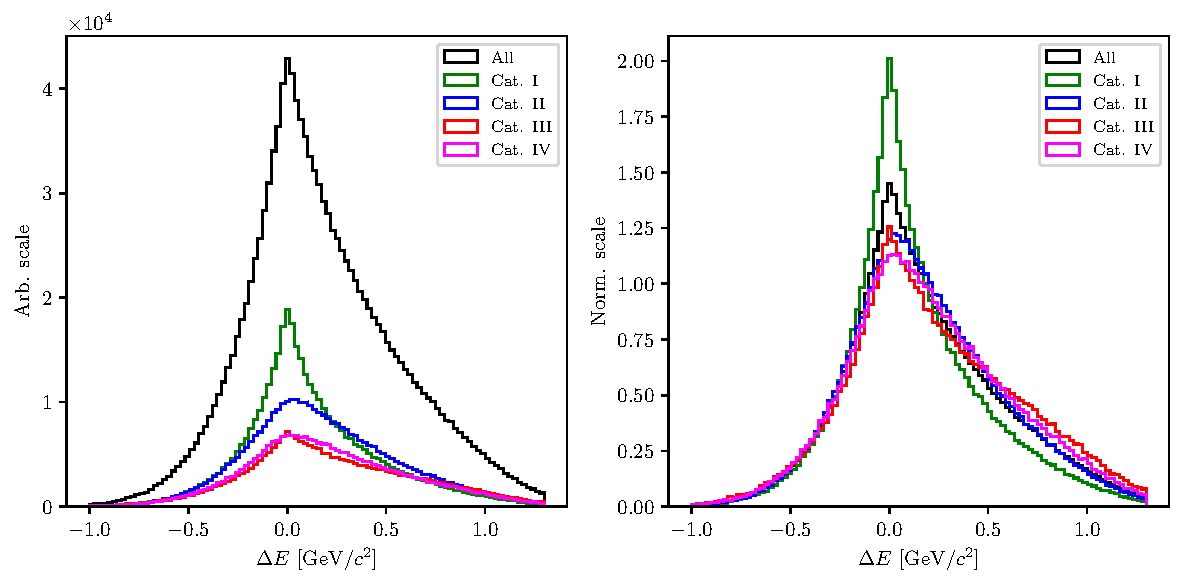
\includegraphics[width=\linewidth]{fig/sig_categ}
\caption{Categorization of signal candidates based on the charge product of both $B$ mesons in the event and the MVA output for recognizing hadronic decays of the companion $B$ meson. The plot on the left shows the distributions in an arbitrary scales, while the plot on the right shows the normalized distributions.}
\label{fig:sig_categ}
\end{figure}


\subsection{Hadronic decay MVA training}
\label{subs:HDMVA}

In order to train an MVA classifier to recognize events with hadronically decaying $B$ mesons in the ROE side, we prepare a dataset of
\begin{itemize}
\item 249385 target candidates,
\item 223681 background candidates,
\end{itemize}
where the definition of target is a ROE which corresponds to a hadronically decayed companion $B$ meson. 

The input variables used in this MVA are ROE specific and do not depend on the signal side. They are
\begin{itemize}
\item angle between tracks,
\item track quantities
	\begin{itemize}
	\item $P(\chi^2,DOF)$ of the tracks fit from the ROE side,
	\item $K$ and $\ell$ FlavorTagger variables,
	\item Charge of the ROE,
	\item $\cos \theta$ of the ROE momentum in the CMS frame,
	\item Number of tracks in ROE,
	\item Number of distant tracks in ROE, which don't pass requirements from Section \ref{s:ss}.
	\end{itemize}
\end{itemize}
%
The classifier output is shown in Figure \ref{fig:hdmva} (left). Candidates which populate the region with low values of the classifier output are more likely to come from semi-leptonic decays, so we want to discard those candidates. When optimizing the $FOM$, we redefine the $S$ in Eq. (\ref{eq:fom}) to a correctly reconstructed signal candidate with a hadronically decayed companion $B$ meson. This $FOM$ optimization, shown in Figure \ref{fig:hdmva} (right), yields the optimal cut
\begin{itemize}
\item $BDT_{had.} > 0.57.$
\end{itemize} 

\begin{figure}[H]
\centering
\captionsetup{width=0.8\linewidth}
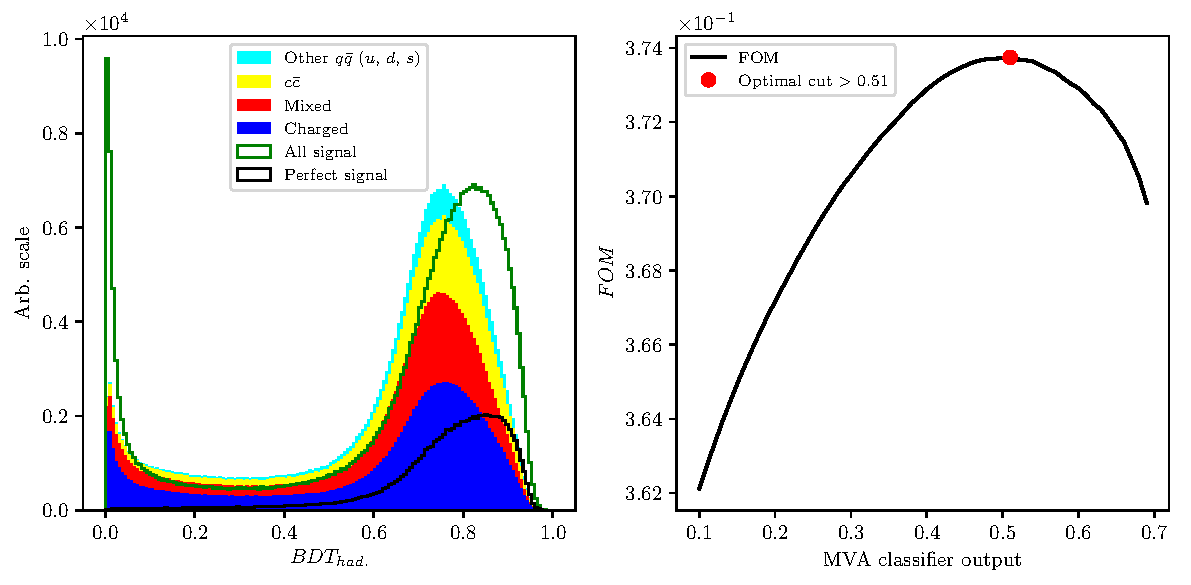
\includegraphics[width=\linewidth]{fig/hdmva_opt}
\caption{Hadronic MVA classifier output for major types of background and scaled-up signal (left), and $FOM$ optimization on this cut for correctly reconstructed signal candidates with hadronically decayed companion $B$ meson (right).}
\label{fig:hdmva}
\end{figure}

\section{Signal region definition}

Since signal candidates are now categorized, we can define a signal region, where most of our perfectly reconstructed candidates lie. We use this region for optimizations of all cuts in the following steps of background suppression in chapter \ref{sec:background-suppression}. The 2D $FOM$ optimization of the optimal $M_{BC}$ and $\Delta E$ is shown in Figure \ref{fig:sigwin}.
The signal region is defined as
\begin{itemize}
\item $M_{BC} > 5.270\e{GeV}/c^2.$,
\item $\vert \Delta E \vert < 0.166\e{Gev}$. 
\end{itemize}

\begin{figure}[H]
\centering
\captionsetup{width=0.8\linewidth}
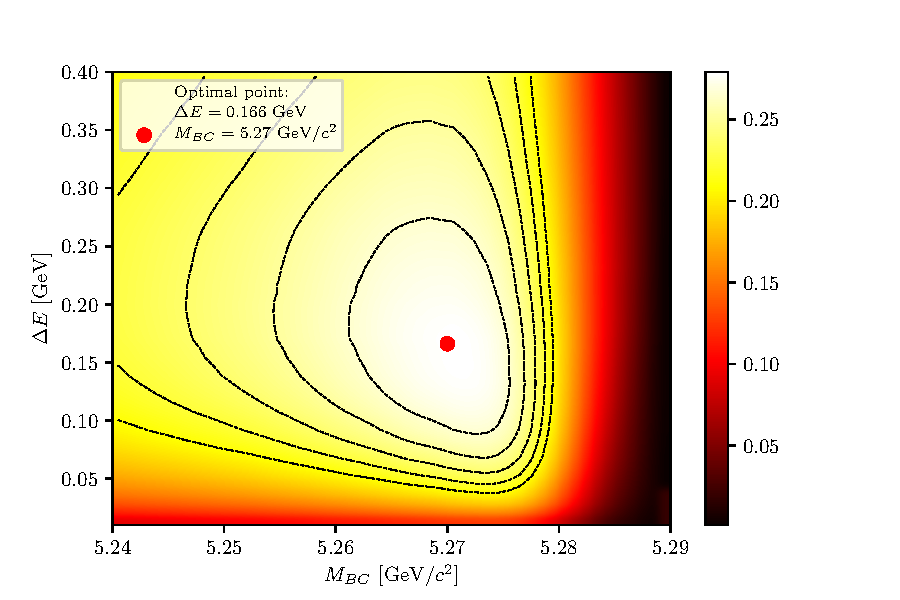
\includegraphics[width=\linewidth]{fig/sigWin}
\caption{2D $FOM$ optimization of the signal region definition, where the signal in the optimization was represented by perfectly reconstructed candidates.}
\label{fig:sigwin}
\end{figure}

Lastly, we can tighten the cut on $m_{miss}^2$, which we intentionally left loose before the signal categorization. With the $FOM$ optimization of perfectly reconstructed candidates inside the signal region, shown in Figure \ref{fig:missm2opt}, the optimal cut on $m_{miss}^2$ is 

\begin{itemize}
\item $\vert m_{miss}^2 \vert < 1.1\e{GeV}/c^2$.
\end{itemize}

\begin{figure}[H]
\centering
\captionsetup{width=0.8\linewidth}
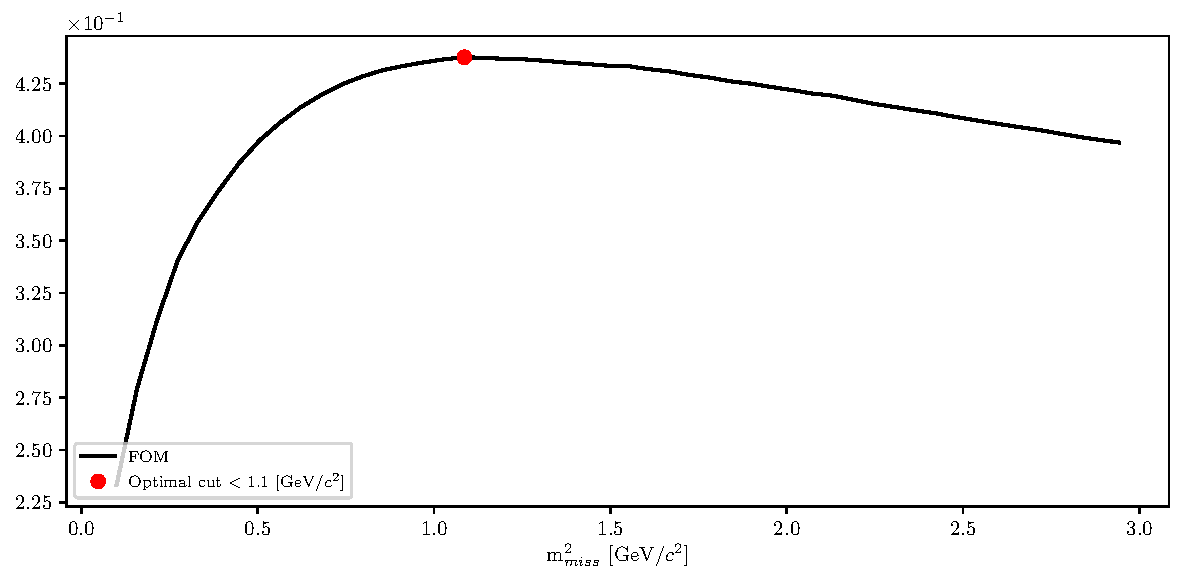
\includegraphics[width=\linewidth]{fig/missm2_opt}
\caption{$FOM$ optimization of the optimal $m_{miss}^2$ cut in the signal region.}
\label{fig:missm2opt}
\end{figure}

\section{Selection summary}
\label{s:ss}
In this section one can find the summary of all selection cuts in the event reconstruction, from FSP particles up to the $B$ meson.

\begin{itemize}
\item FSP particles:
	\begin{itemize}
	\item Electrons: $\vert d_0 \vert < 0.1\e{cm},\,\vert z_0 \vert < 1,5\e{cm},\,p>0.6\e{GeV}/c,\\p_{CMS}\in[0.4,\,2.6]\e{GeV}/c,\,eID>0.9,$
    \item Muons: $\vert d_0 \vert < 0.1\e{cm},\,\vert z_0 \vert < 1,5\e{cm},\,p_{CMS}\in[0.6,\,2.6]\e{GeV}/c,\\\mu ID>0.97,$
    \item Kaons: $\vert d_0 \vert < 0.15\e{cm},\,\vert z_0 \vert < 1,5\e{cm},\,p_{CMS} < 2.5\e{GeV}/c,\\K/\pi~ID>0.6,\,K/p~ID>0.1,$
	\end{itemize}
\item $B$ meson candidates:
	\begin{itemize}
	\item Before ROE clean-up: $P(\chi^2,\,DOF) > 1\E{-3},\,\vert \cos \theta_{BY} \vert < 1,\,\vert m_{miss}^2 \vert < 7\e{GeV}/c^2,$
    \item After ROE clean-up: $\Delta E \in [-1.0,1.3]\e{GeV},\,M_{BC} \in [5.1,5.295]\e{GeV}/c^2,$
    \item After signal categorization: $q_{B_{sig}}~q_{B_{comp}} = -1,\,BDT_{had.} > 0.51,\,\vert m_{miss}^2\vert<~1.1\e{GeV}/c^2.$
	\end{itemize}
\end{itemize}

\chapter{Rest of event clean-up}
\label{ch:roe}

Continuing from Section \ref{sec:loose-neutrino-reconstruction}, the description of the ROE clean-up process is described here. 

\section{Setting up the MVA}

Training the MVA classifiers follows the same recipe for all the steps in this chapter. For each step we run $B$ meson reconstruction on Signal MC with a generic companion $B$ meson. This way the produced weight files are less likely to be signal-side dependent and can be used also for untagged analyses of other decays. For every correctly reconstructed signal $B$ meson we save the necessary information for each MVA step (i.e. properties of ROE clusters). Only correctly reconstructed candidates are chosen here, to prevent leaks of information from the signal side to the ROE side.

For each clean-up step a dataset was prepared for the training of "signal" (target) against "background". The Fast-BDT (FBDT) \cite{keck2017fastbdt} algorithm was used as the MVA classifier and the following hyper-parameters were chosen for optimization
\begin{itemize}
\item \texttt{nTrees}: the number of trees in the FBDT forest,
\item \texttt{nLevels}: the number of levels in each FBDT tree.
\end{itemize}

Figure \ref{fig:BDT} shows a graphical interpretation of the FBDT forest with \texttt{nTrees} and \texttt{nLevels}. In all cases the hyper-parameters were optimized with a grid-search method in the hyper-parameter phase-space. Additionally, we perform a $k$-fold cross-validation ($k=5$) for each hyper-parameter set, where we cycle through the $5$ parts of the dataset and use $4$ parts of the dataset for training, whereas the remaining part is used for validation. This minimizes the bias towards the validation sample when optimizing the hyper-parameters.

\begin{figure}[H]
\centering
\captionsetup{width=0.8\linewidth}
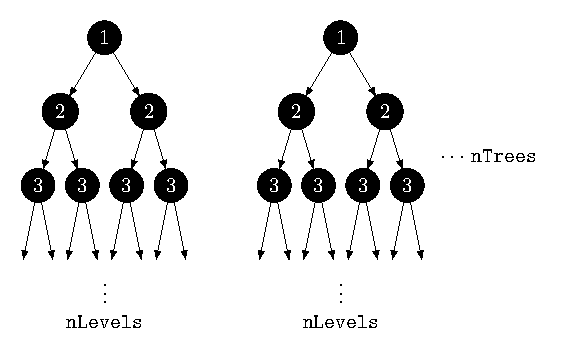
\includegraphics[scale=1]{texfig/BDT_forest}
\caption{A schematic of a BDT forest with \texttt{nTrees}, each tree having a depth of \texttt{nLevels}.}
\label{fig:BDT}
\end{figure}

\section{Clusters clean-up}

Photons originate from the IP region, travel to the ECL part of the detector in a straight line and produce a cluster. The direction of the photon is determined via the location of the cluster hit in the ECL and the energy of the photon is directly measured via the deposited energy. This way the four-momentum of photons is determined and used in Eq. (\ref{eq:ROEloop}).

Most of the photons in events with $B$ mesons come from $\pi^0 \to \gamma \gamma$ decays. However, a lot of hits in the ECL are also created by photons coming from beam-induced background or secondary interactions with the detector material. Such photons add extra energy and momentum which spoils our measured quantities.

In the first step of the clusters clean-up we train an MVA which recognizes good $\pi^0$ candidates. The output of this classifier is then applied to photons and represents a sort of a $\pi^0$ origin probability, which is used as an additional classifier variable in the next step of the clean-up.

\subsection{$\pi^0$ MVA training}

The dataset of $\pi^0$ candidates contains
\begin{itemize}
\item 387125 target candidates,
\item 416019 background candidates,
\end{itemize}
where the definition of target is that both photon daughters that were used in the reconstruction of the $\pi^0$ are actual photons and real daughters of the $\pi^0$ particle. We use $\pi^0$ candidates from the converted Belle particle list and select those with invariant mass in the range of $M \in [0.10,~0.16]\e{GeV}$. After that we perform a mass-constrained fit on all candidates, keeping only the ones for which the fit converged. 

The input variables used in this MVA are
\begin{itemize}
\item $p$ and $p_{CMS}$ of $\pi^0$ and $\gamma$ daughters,
\item fit prob. of the mass-constrained fit, invariant mass and significance of mass before and after the fit,
\item angle between the photon daughters in the CMS frame,
\item cluster quantities for each daughter photon
	\begin{itemize}
	\item $E_9/E_{25}$,
	\item theta angle,
	\item number of hit cells in the ECL,
	\item highest energy in cell,
	\item energy error,
	\item distance to closest track at ECL radius.
	\end{itemize}
\end{itemize}

The classifier output variable is shown in Figure \ref{fig:ROE_pi0}.

\begin{figure}[H]
\centering
\captionsetup{width=0.8\linewidth}
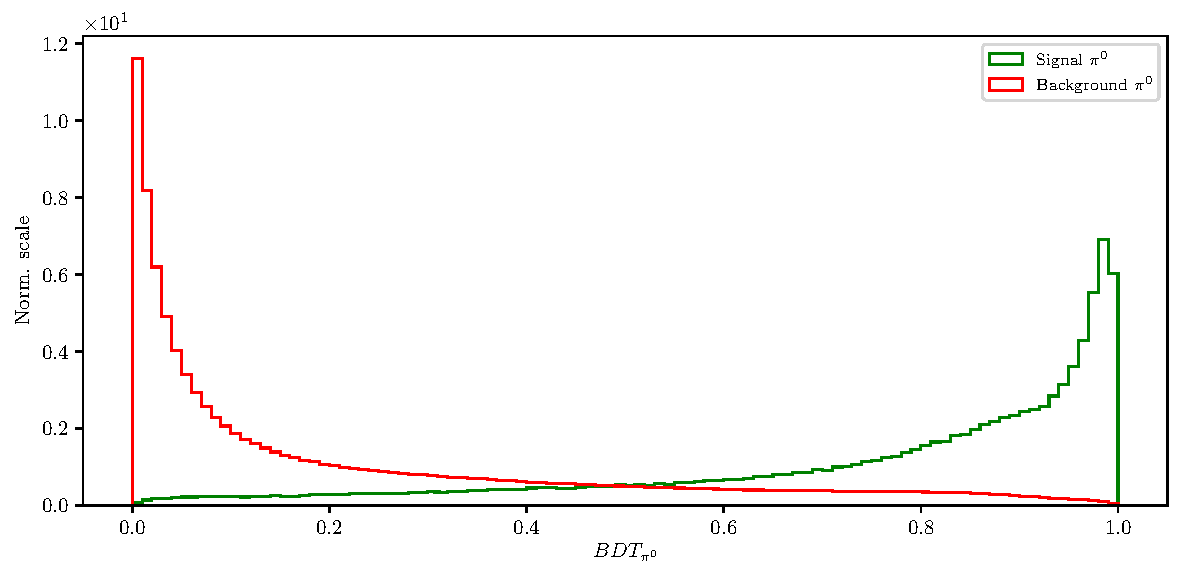
\includegraphics[width=\linewidth]{fig/ROECleanup_pi0}
\caption{Classifier output of the $\pi^0$ training for signal and background $\pi^0$ candidates.}
\label{fig:ROE_pi0}
\end{figure}

The distributions for all input variables and their correlations for signal and background candidates can be found in Appendix X for all steps of the ROE clean-up.


\subsection{$\gamma$ MVA training}

In this MVA training we take the $\pi^0$ classifier output of the previous training as an input in order to train a classifier to distinguish between good and bad photons. The $\pi^0$ probability information from the previous step is applied to all photon pairs which pass the same $\pi^0$ cuts as defined in the previous step. Since it's possible to have overlapping pairs of photons, the $\pi^0$ probability is overwritten in the case of a larger value, since this points to a greater probability of a correct photon combination. On the other hand, some photon candidates fail to pass the $\pi^0$ selection, these candidates have a fixed value of $\pi^0$ probability equal to zero.

The dataset of $\gamma$ candidates contains
\begin{itemize}
\item 324781 target candidates,
\item 333353 background candidates,
\end{itemize}
where the definition of target is that the photon is an actual photon which is related to a primary MC particle. This tags all photon particles from secondary interactions as background photons. We use the converted $\gamma$ candidates from the existing Belle particle list. 

The input variables used in this MVA are
\begin{itemize}
\item $p$ and $p_{CMS}$ of $\gamma$ candidates,
\item $\pi^0$ probability,
\item cluster quantities
	\begin{itemize}
	\item $E_9/E{25}$,
	\item theta angle,
	\item number of hit cells in the ECL,
	\item highest energy in cell,
	\item energy error,
	\item distance to closest track at ECL radius.
	\end{itemize}
\end{itemize}

The classifier output variable is shown in Figure \ref{fig:ROE_gamma}.

\begin{figure}[H]
\centering
\captionsetup{width=0.8\linewidth}
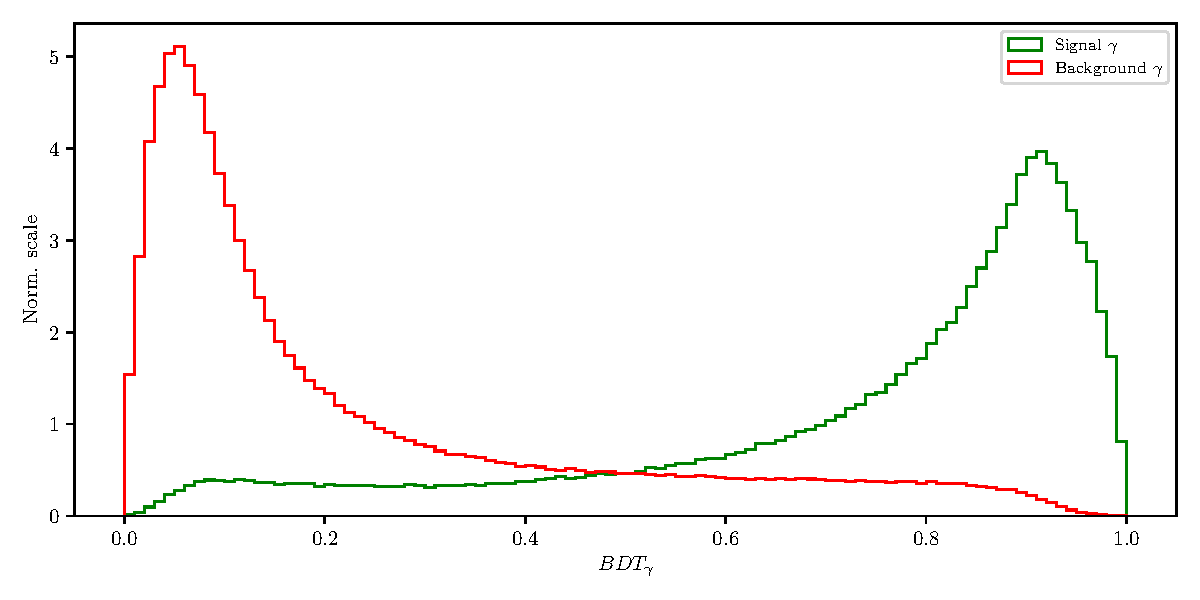
\includegraphics[width=\linewidth]{fig/ROECleanup_gamma}
\caption{Classifier output of the $\gamma$ training for signal and background $\gamma$ candidates.}
\label{fig:ROE_gamma}
\end{figure}

With the final weights for photon classification in hand, we apply them to the photon particle list. The cut optimization is shown in Figure \ref{fig:ROE_gamma_opt} (left), with the optimal cut on the $\gamma$ classifier output at
\begin{itemize}
\item $BDT_\gamma > 0.519$.
\end{itemize}

Figure \ref{fig:ROE_gamma_opt} (right) shows the LAB frame momentum of the photons before and after the cut in logarithmic scale. The signal efficiency and background rejection at this clean-up cut are
\begin{itemize}
\item Signal efficiency: $\epsilon_{SIG} = 82.6~\%$,
\item Background rejection: $1-\epsilon_{BKG} = 81.7~\%$.
\end{itemize}

\begin{figure}[H]
\centering
\captionsetup{width=0.8\linewidth}
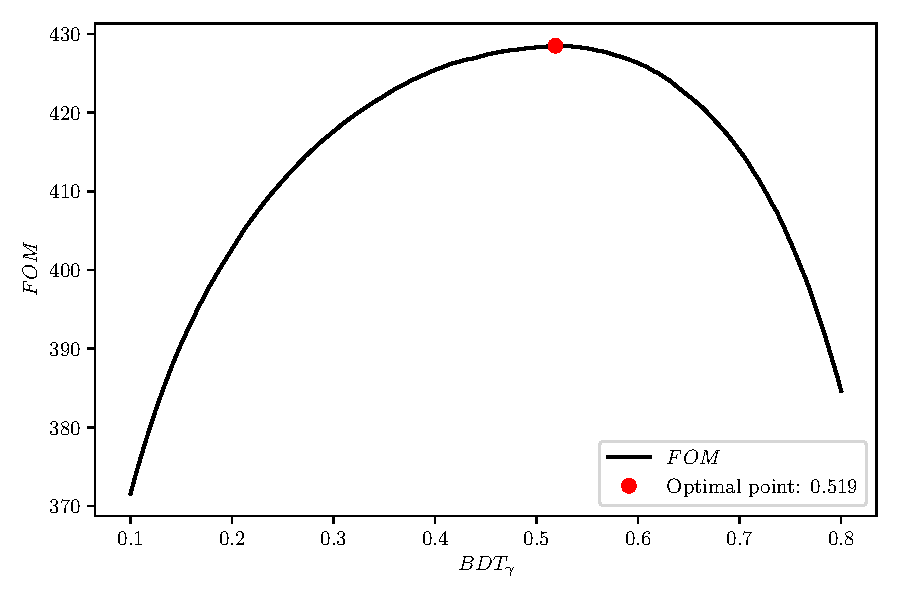
\includegraphics[width=\linewidth]{fig/ROECleanup_gamma_opt}
\caption{The $FOM$ of the classifier output optimization (left) and  momentum magnitude in the LAB frame of signal and background photon candidates before and after the optimal cut (right).}
\label{fig:ROE_gamma_opt}
\end{figure}

The event is now considered to be clean of extra clusters.

\section{Tracks clean-up}

Charged particles leave hits in the detector, which are then grouped into tracks by advanced tracking algorithms. The track is fitted and the track momentum is determined. With the help of particle identification information (PID), we are able to make an intelligent decision about the mass hypothesis of the particle and thus reconstruct the charged particle's four-momentum, which is then added in the loop in Eq. (\ref{eq:ROEloop}).

Most of the quality (good) tracks, which come from physics event of interest, come from the IP region, where the collisions occur. Cleaning up the tracks is a more complex procedure than cleaning up the clusters. The following facts need to be taken into account
\begin{enumerate}[(a)]
\item good tracks can also originate away from the IP region, due to decays of long-lived particles, such as $K_S^0 \to \pi^+ \pi^-$,
\item charged particles from background sources produce extra tracks, or duplicates,
\item low momentum charged particles can curl in the magnetic field and produce multiple tracks,
\item secondary interactions with detector material or decays of particles in flight can produce "kinks" in the flight directory, resulting in multiple track fit results per track.
\end{enumerate}

Schematics of all the cases mentioned above are shown in Figure \ref{fig:track_cleanup}.

\begin{figure}[H]
\centering
\subfigure[]{
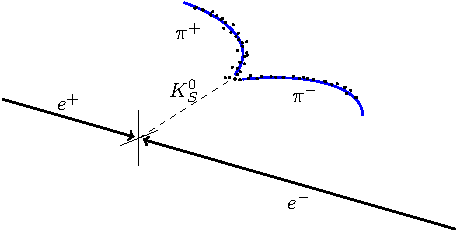
\includegraphics[width=0.49\linewidth]{texfig/V0}}%
\subfigure[]{
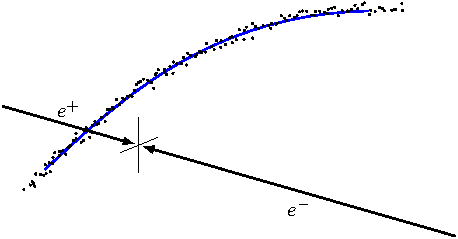
\includegraphics[width=0.49\linewidth]{texfig/background}}\\
\subfigure[]{
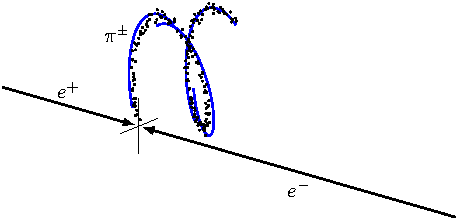
\includegraphics[width=0.49\linewidth]{texfig/curler}}%
\subfigure[]{
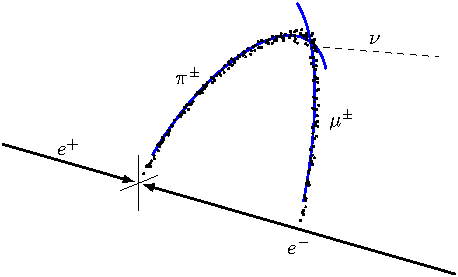
\includegraphics[width=0.49\linewidth]{texfig/decay}}%
\caption{(a) Tracks from long-lived neutral particles, which decay away from the IP region, (b) Random tracks from background which are reconstructed, (c) Low-momentum particles which curl in the magnetic field, (d) in-flight decays of particles, which produce a kink in the trajectory.}
\label{fig:track_cleanup}
\end{figure}

It is obvious that tracks from the same momentum source should only be taken into account once, or, in case of background tracks, not at all. Such tracks will from this point on be denoted as \textit{extra} tracks, because they add extra four-momentum to our final calculations in Eq. (\ref{eq:ROEloop}). At the same time, we have to take care that we don't identify \textit{good} tracks as \textit{extra} tracks. Both of these cases have negative impacts on the final resolution of all variables which depend on information from ROE.

\subsection{Tracks from long-lived particles}

The first step in tracks clean-up is taking care of tracks from long-lived particles. Here we only focus on $K_S^0$, since they are the most abundant. This step is necessary because the $\pi^\pm$ particles, coming from the $K_S^0$ decays, have large impact parameters, which is usually a trait of background particles. In order to minimize confusion from the MVA point-of-view, these tracks are taken into account separately.

We use the converted $K_S^0$ candidates from the existing Belle particle list and use a pre-trained Neural Network classifier result in order to select only the good $K_S^0$ candidates. Figure \ref{fig:ROE_V0} shows the distribution of the $K_S^0$ invariant mass for signal and background candidates, before and after the classifier cut. The momentum of selected $K_S^0$ candidates is added to the ROE, while the daughter tracks are discarded from our set.

\begin{figure}[H]
\centering
\captionsetup{width=0.8\linewidth}
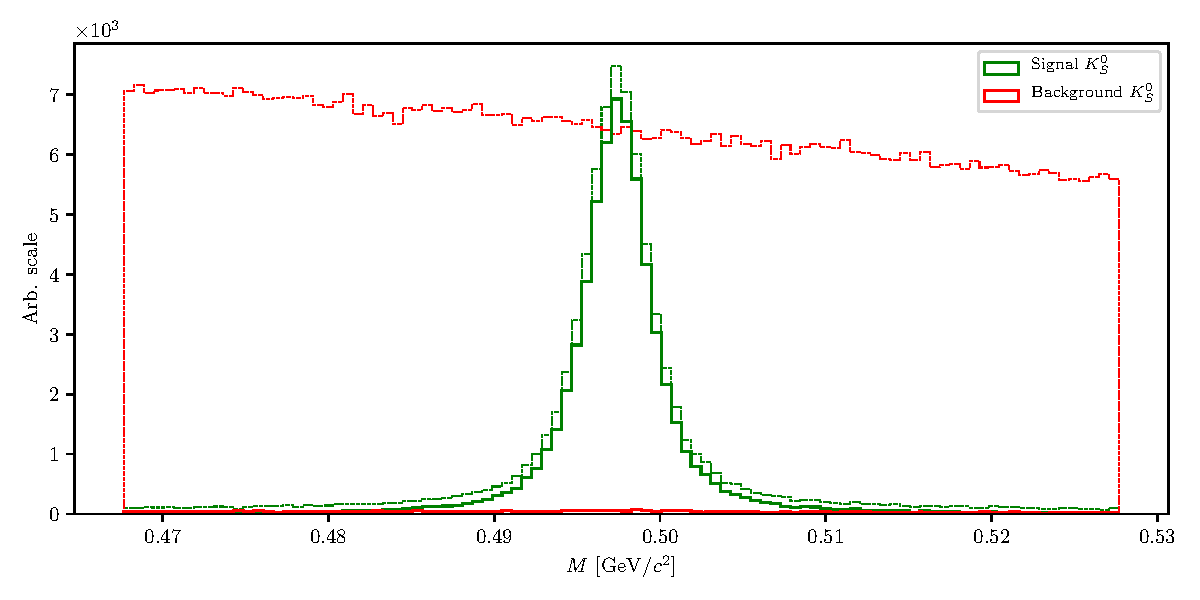
\includegraphics[width=\linewidth]{fig/ROECleanup_V0}
\caption{Invariant mass of the $K_S^0$ candidates before (dashed lines) and after (solid lines) the cut on the Neural Network classifier for signal (green) and background candidates (red). Signal peaks at nominal $K_S^0$ mass, while background covers a wider region.}
\label{fig:ROE_V0}
\end{figure}

The signal efficiency and background rejection for $K_S^0$ candidates after this cut and on the full range are
\begin{itemize}
\item Signal efficiency: $\epsilon_{SIG} = 80.7~\%$,
\item Background rejection: $1-\epsilon_{BKG} = 99.4~\%$.
\end{itemize}

\subsection{Duplicate tracks}
All good tracks at this point should be coming from the IP region, since we took care of all the good tracks from long-lived particle decays, therefore we apply a cut on impact parameters for all the remaining tracks
\begin{itemize}
\item $\vert d_0 \vert < 10\e{cm}$ and $\vert z_0 \vert < 20\e{cm}$
\end{itemize} 

and proceed with the clean-up of track duplicates.

\subsubsection{Defining a duplicate track pair}

In this step we wish to find a handle on secondary tracks from low momentum curlers and decays in flight. The main property for these cases is that the angle between such two tracks is very close to $0^\circ$ or $180^\circ$, since tracks deviate only slightly from the initial direction, but can also be reconstructed in the opposite way. Figure \ref{fig:ROE_dupAngleInit} shows the distribution of the angle between two tracks in a single pair for random track pairs and duplicate track pairs, where the latter were reconstructed as two same-sign or opposite-sign tracks.

\begin{figure}[H]
\centering
\captionsetup{width=0.8\linewidth}
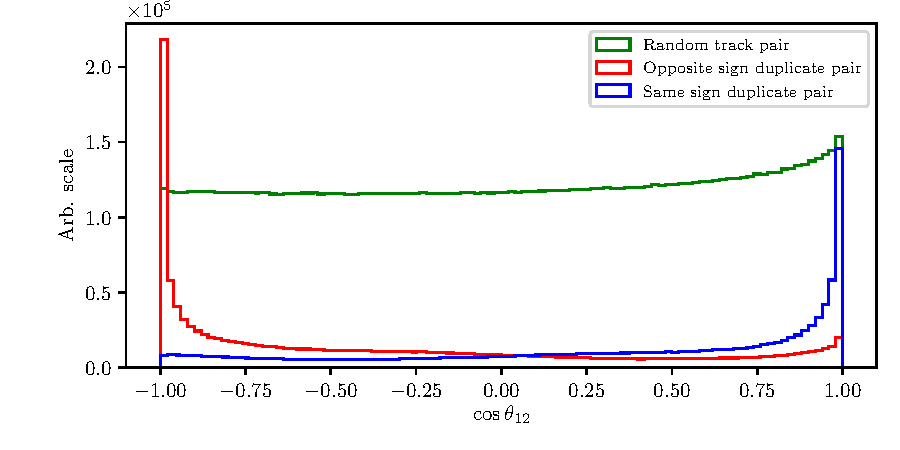
\includegraphics[width=\linewidth]{fig/ROECleanup_dup_angle_initial}
\caption{Distribution of the angle between two tracks in a single pair for random track pairs (green) and duplicate track pairs, where the latter were reconstructed as two same-sign (blue) or opposite-sign tracks (red).}
\label{fig:ROE_dupAngleInit}
\end{figure}

If the particle decayed mid-flight or produced multiple tracks due to being a low-momentum curler, then, as the name suggests, these particles most likely had low momentum in the transverse direction, $p_T$. Since both tracks originate from the same initial particle, the momentum difference should also peak at small values. Figure \ref{fig:ROE_dupPt} shows the momentum and momentum difference of tracks which belong to a random or a duplicate track pair.

\begin{figure}[H]
\centering
\captionsetup{width=0.8\linewidth}
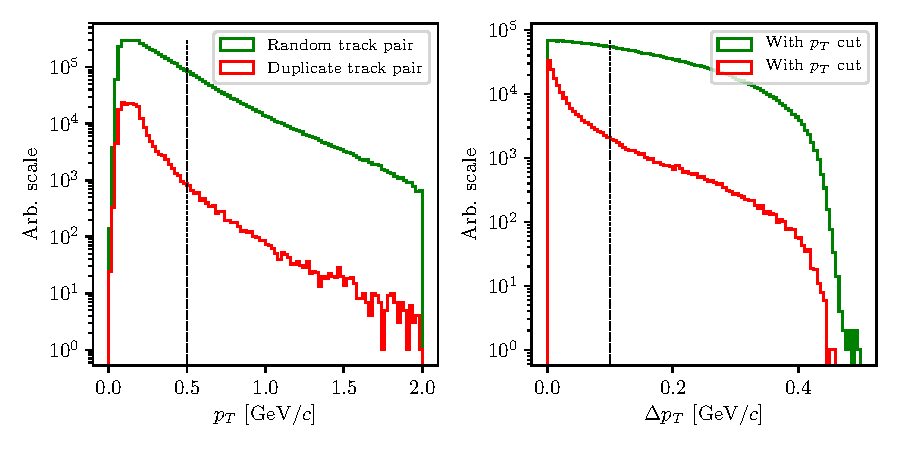
\includegraphics[width=\linewidth]{fig/ROECleanup_dup_pt}
\caption{Distribution of transverse momentum $p_T$ (left) and transverse momentum difference $\Delta p_T$ (right) for all tracks coming from random (green) or duplicate track pairs (red). The plot on the right already includes the cut on $p_T$ from the plot on the left.}
\label{fig:ROE_dupPt}
\end{figure}

We impose a cut of
\begin{itemize}
\item $p_T < 0.5\e{GeV}/c$,
\item $\vert \Delta p_T \vert < 0.1\e{GeV}/c$,
\end{itemize}

in order to cut down the number of random track pairs, while retaining a high percentage of duplicate track pairs. After all the cuts defined in this chapter, the final distribution of the angle between two tracks is shown in Figure \ref{fig:ROE_dupAngleFinal}.

\begin{figure}[H]
\centering
\captionsetup{width=0.8\linewidth}
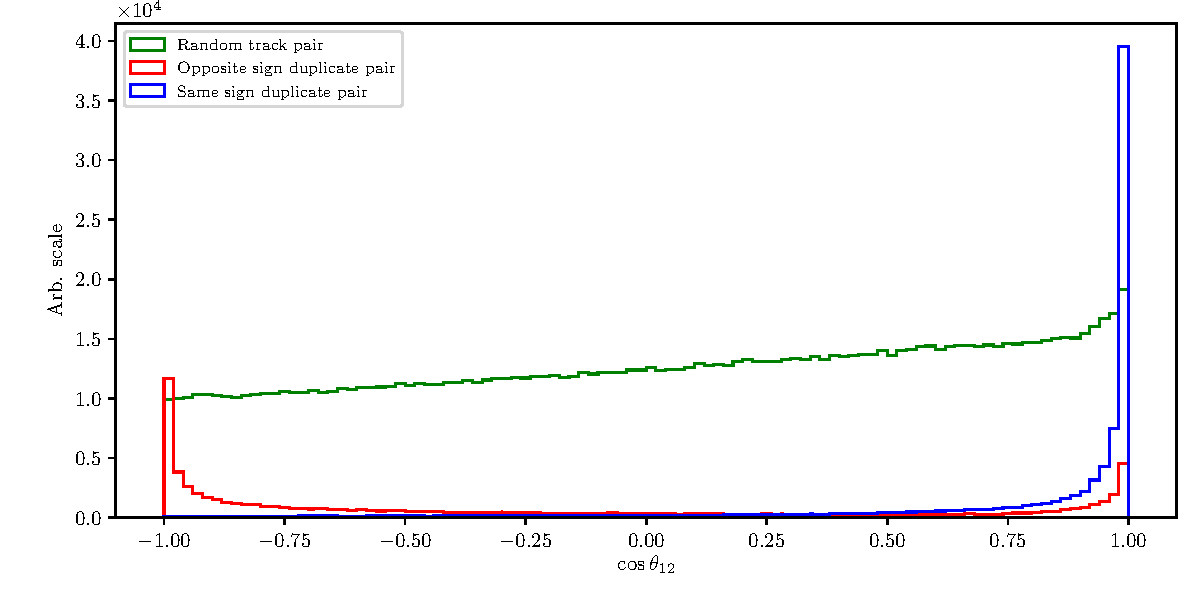
\includegraphics[width=\linewidth]{fig/ROECleanup_dup_angle_final}
\caption{Distribution of the angle between two tracks in a single pair after applying the selection cuts defined in this subsection. The distributions are shown for random track pairs (green) and duplicate track pairs, where the latter were reconstructed as two same-sign (blue) or opposite-sign tracks (red).}
\label{fig:ROE_dupAngleFinal}
\end{figure}

\subsubsection{Training the duplicate track pair MVA}
\label{ss:trackMVA}

This final sample of track pairs is now fed into an MVA, which is trained to recognize duplicate track pairs over random ones. The dataset contains
\begin{itemize}
\item 215601 target candidates,
\item 311124 background candidates,
\end{itemize}
where the definition of target is that the track pair is a duplicate track pair. 

The input variables used in this MVA are
\begin{itemize}
\item angle between tracks,
\item track quantities
	\begin{itemize}
	\item impact parameters $d_0$ and $z_0$,
	\item transverse momentum $p_T$,
	\item helix parameters and helix parameter errors of the track,
	\item track fit $p$-value,
	\item number of hits in the SVD and CDC detectors
	\end{itemize}
\end{itemize}

The classifier is able to distinguish between random and duplicate track pairs in a very efficient manner, as shown in Figure \ref{fig:ROE_dupBDT}.

\begin{figure}[H]
\centering
\captionsetup{width=0.8\linewidth}
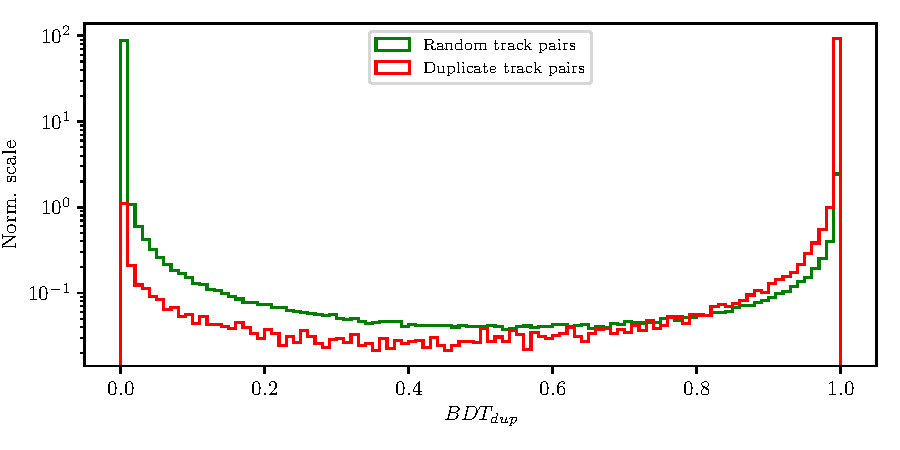
\includegraphics[width=\linewidth]{fig/ROECleanup_dup}
\caption{Classifier output of the track pair training for random track pairs and duplicate track pairs.}
\label{fig:ROE_dupBDT}
\end{figure}

The $FOM$ function for optimal cut selection is shown in Figure \ref{fig:ROE_dupOpt} (left), along with the angle between the two tracks before and after the optimal cut (right). The optimal cut for duplicate track selection is
\begin{itemize}
\item $BDT_{duplicate} > 0.99915.$
\end{itemize}

\begin{figure}[H]
\centering
\captionsetup{width=0.8\linewidth}
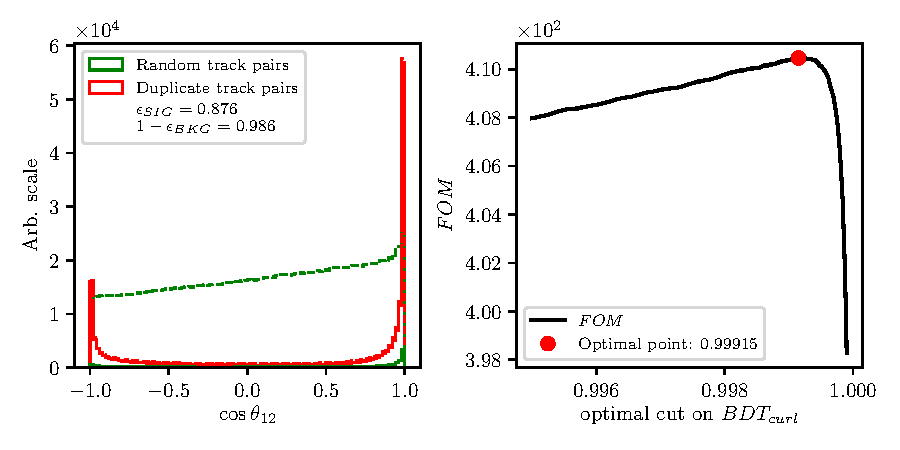
\includegraphics[width=\linewidth]{fig/ROECleanup_dup_opt}
\caption{The optimization of the FOM function for the cut on classifier output (left) and distribution of the angle between two tracks in a single pair before (dashed) and after (solid) applying the optimal cut on the output classifier for random and duplicate track pairs (right).}
\label{fig:ROE_dupOpt}
\end{figure}

\subsubsection{Defining duplicate tracks}

What remains now is to decide which track from the duplicate track pair to keep and which to discard. For this purpose we apply duplicate pair-level information to each track in the pair in the form of
\begin{equation}
\Delta f = f_{this} - f_{other},
\end{equation}

where $f$ is an arbitrary variable from the list of track quantities in Subsection \ref{ss:trackMVA}. From the point-of-view of \textit{this} track, a track is more $duplicate$-like if the following is true
\begin{itemize}
\item $\Delta d_0,\,\Delta z_0 > 0$ (\textit{this} track further away from the IP region),
\item $\Delta p_T,\,\Delta p_Z < 0$ (\textit{this} track has lower momentum),
\item $\Delta N_{SVD},\,\Delta N_{CDC} < 0$ (\textit{this} track has less hits in the SVD and CDC),
\end{itemize}

Additionally we define an MC truth variable 
\begin{equation}
\label{eq:chi2}
\Delta \chi^2 = \chi^2_{this} - \chi^2_{other},\quad\chi^2 = \sum_{i=x,y,z}\frac{\left(p_i - p_i^{MC}\right)^2}{\sigma(p_i)^2},
\end{equation}
where we compare all components of track momentum to the true values. If $\Delta \chi^2 > 0$, then \textit{this} track has a higher probability of being a duplicate track and should be discarded.

However, it turns out that solving this problem is not as simple as discarding one track and keeping the other one. An additional complication here is that we can have more than one extra track from the same initial particle, which leads to track pairs where both tracks are track duplicates. For example, if we have the following case
\begin{align*}
t_1&: \mathrm{good~track},\\
t_2&: \mathrm{extra~track},\\
t_3&: \mathrm{extra~track},\\
\mathrm{pair}_1&:\left(t_1,t_2\right),\\
\mathrm{pair}_2&:\left(t_1,t_3\right),\\
\mathrm{pair}_3&:\left(t_2,t_3\right),
\end{align*}
where $t_1$ is the original track and $t_2$ and $t_3$ are extra tracks, with $t_3$ being even more duplicate-like with respect to $t_2$. Here tracks $t_2$ and $t_3$ should be discarded while $t_1$ should be kept. We can achieve this if we overwrite existing pair-level information in the tracks for cases where the variable difference $\Delta f$ is more duplicate-like. If we follow the same example, we could fill information about the property $f$ in six different orders. 
\begin{align*}
1.&~\left(t_1,t_2*\right)\quad \to \quad \left(t_1,t_3*\right)\quad \to \quad \left(t_2*,t_3*\right),\\ 
2.&~\left(t_1,t_2*\right)\quad \to \quad \left(t_2*,t_3*\right)\quad \to \quad \left(t_1,t_3*\right),\\ 
3.&~\left(t_1,t_3*\right)\quad \to \quad \left(t_2,t_3*\right)\quad \to \quad \left(t_1,t_2*\right),\\
4.&~\left(t_1,t_3*\right)\quad \to \quad \left(t_1,t_2*\right)\quad \to \quad \left(t_2*,t_3*\right),\\
5.&~\left(t_2,t_3*\right)\quad \to \quad \left(t_1,t_3*\right)\quad \to \quad \left(t_1,t_2*\right),\\
6.&~\left(t_2,t_3*\right)\quad \to \quad \left(t_1,t_2*\right)\quad \to \quad \left(t_1,t_3*\right),
\end{align*}

where the "*" symbol denotes when a track is recognized as a duplicate track with respect to the other track. We see that no matter the order, both $t_2$ and $t_3$ get recognized as duplicate tracks correctly.

\subsubsection{Training the duplicate track MVA}
The training procedure is similar as before. The sample of tracks from duplicate track pairs is now fed into an MVA, which is trained to distinguish duplicate tracks from good tracks. The dataset contains
\begin{itemize}
\item 160146 target candidates,
\item 128568 background candidates,
\end{itemize}
where the definition of target is that the track is a duplicate track. 

The input variables used in this MVA are
\begin{itemize}
\item theta angle of the track momentum,
\item track quantities
	\begin{itemize}
	\item impact parameters $d_0$ and $z_0$,
	\item momentum components $p_T$ and $p_z$
	\item number of hits in the SVD and CDC detectors
	\item track fit $p$-value,
	\end{itemize}
\item pair-level information
	\begin{itemize}
	\item $\Delta d_0$, $\Delta z_0$, $\Delta N_{CDC}$, $\Delta N_{SVD}$, $\Delta p_T$, $\Delta p_z$.  
	\end{itemize}
\end{itemize}

The classifier is shown in Figure \ref{fig:ROE_curl}. The weights from this training are applied to the tracks, where now each track has a certain probability of being a duplicate track. We now compare these values between both tracks in each track pair as
\begin{equation}
\Delta BDT_{final} = BDT_{final}^{this} - BDT_{final}^{other},
\end{equation}

which is again applied to all track pairs and overwritten for tracks which are more duplicate-like.

\begin{figure}[H]
\centering
\captionsetup{width=0.8\linewidth}
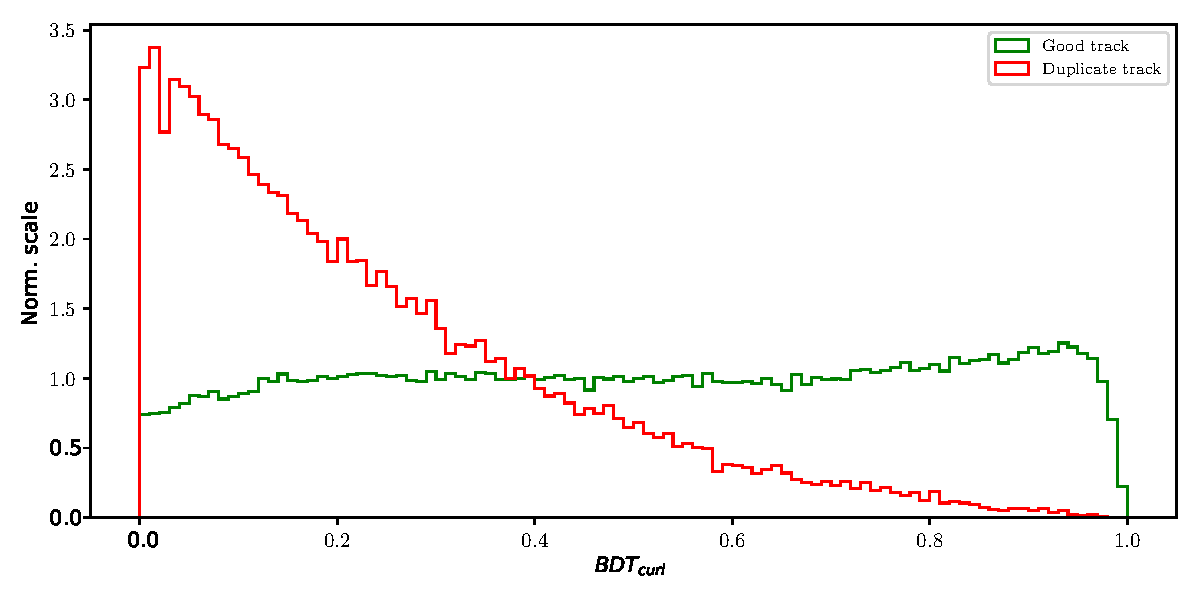
\includegraphics[width=\linewidth]{fig/ROECleanup_curl}
\caption{Classifier output of the MVA training for curling track recognition.}
\label{fig:ROE_curl}
\end{figure}

Finally, we select all duplicate tracks which survive the cut 
\begin{equation}
\Delta BDT_{final} > 0
\end{equation}

and discard them from our ROE. We can check the performance of our duplicate track classifier by applying the procedure on a sample of duplicate track pairs and comparing the predicted result with the truth, based on Eq. (\ref{eq:chi2}). Table \ref{tab:rat} shows the performance of the duplicate track recognition in the form of percentages of correctly and incorrectly identified duplicate and original tracks. The model seems to perform well and the event is now considered to be clean of duplicate tracks.

\begin{table}[H]
\centering
\begin{tabular}{|c|c|c|}
\hline
 & Predicted duplicate track & Predicted good track \\
 \hline 
 Duplicate track & $84.63~\%$  & $20.95~\%$  \\
 \hline
 Good track & $15.37~\%$ & $79.05~\%$ \\
 \hline
\end{tabular}
\caption{Ratios of correctly classified and misclassified tracks.}
\label{tab:rat}
\end{table}

\section{Belle clean-up}

The clean-up, used standardly at Belle, is much simpler and relies only on a set of rectangular cuts for neutral particles as well as charged ones. In case of photons, a single cut on photon energy is applied, depending on the region where the photon hit the relevant part of the detector. The photon cuts are summarized in Table \ref{tab:bellegamma}.

\begin{table}[H]
\centering
\begin{tabular}{|c|c|c|c|}
\hline
 & $17^\circ < \theta < 32^\circ$ & $32^\circ < \theta < 130^\circ$ & $130^\circ < \theta < 150^\circ$ \\
 \hline 
 $E_\gamma$ & $> 100\e{MeV}$  & $> 50\e{MeV}$ & $> 150\e{MeV}$  \\
 \hline
\end{tabular}
\caption{Photon selection for the Belle clean-up procedure. Different cuts are applied on photons in different parts of the detector}
\label{tab:bellegamma}
\end{table}

In case of tracks, pairs are selected which satisfy the following criteria:
\begin{itemize}
\item $p_T < 275\e{MeV}/c$,
\item $\Delta p = \vert \textbf{p}_1 - \textbf{p}_2\vert  < 100\e{MeV}/c$,
\item $\cos \theta (\textbf{p}_1,\textbf{p}_2) < 15^\circ$ for same sign,
\item $\cos\theta(\textbf{p}_1,\textbf{p}_2) > 165^\circ$ for opposite sign.
\end{itemize}

Of the two tracks, the one with a larger value of formula in Eq. \ref{eq:belleformula} is discarded. The remaining tracks in the event then need to satisfy the conditions described in Table \ref{tab:belletrack}.
\begin{equation}
\label{eq:belleformula}
\left(\gamma\vert d_0 \vert \right)^2 + \vert z_0 \vert^2, \quad \gamma = 5.
\end{equation}

\begin{table}[H]
\centering
\begin{tabular}{|c|c|c|c|}
\hline
 & $p_T < 250\e{MeV}/c$ & $250\e{MeV}/c < p_T < 500\e{MeV}/c$ & $p_T > 500\e{MeV}/c$ \\
 \hline 
 $\vert d_0 \vert$ & $< 20\e{cm}$  & $< 15\e{cm}$ & $< 10\e{cm}$  \\
 \hline
  $\vert z_0 \vert$ & $< 100\e{cm}$  & $< 50\e{cm}$ & $< 20\e{cm}$  \\
  \hline
 
\end{tabular}
\caption{Photon selection for the Belle clean-up procedure. Different cuts are applied on photons in different parts of the detector}
\label{tab:belletrack}
\end{table}

%TODO: preveri vektorje ce so vedno bold

\section{Clean-up results}

In this section the results of the ROE clean-up are shown. It is clear that cleaning up the event affects the shape of various distribution, especially \vars, which we are most interested in. Since the reconstruction procedure includes cuts on the cleaned-up variables, this also results in an efficiency increase of the reconstructed sample. 

We compare the clean-up setup, defined in this analysis, to the standard clean-up used by Belle, and to a default case, where no clean-up was applied at all. Figure \ref{fig:roeopt} shows distributions of \vars~for various clean-up setups. We see an improvement in resolution as well as an increase in efficiency in both observed variables for the case where the ROE clean-up is performed. Table \ref{tab:roeeff} shows ratios of efficiencies and $FWHM$'s of $\Delta E$ with respect to the default case. While both the Belle and ROE clean-up increase efficiency, only ROE clean-up improves the resolution.

%which is the same as our optimal clean-up, with the exception of the masses of FSP particles in Eq. (\ref{eq:pcharged}), which are, in this case, taken from MC. Mass hypothesis determination of charged FSP particles in Eq. (\ref{eq:pcharged}) based on PID information seems to be quite successful, since the benefits of using true masses from Monte Carlo are very small.

\begin{figure}[H]
\centering
\captionsetup{width=0.8\linewidth}
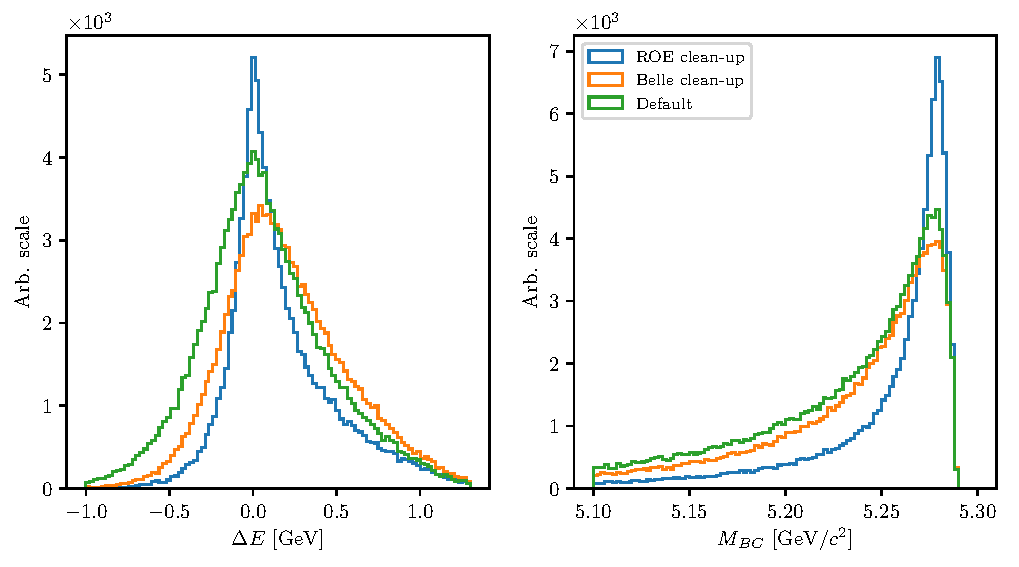
\includegraphics[width=\linewidth]{fig/roe_opt}
\caption{\vars~distributions for various types of clean-up procedures. For ROE clean-up, the procedure seems to improve resolution as well as increase efficiency, compared to the default case.}
\label{fig:roeopt}
\end{figure}

\begin{table}[H]
\centering
\begin{tabular}{|c|c|c|}
\hline
 & Efficiency ratio & FWHM ratio \\
 \hline 
 Belle clean-up & $121.90~\%$  & $102.60~\%$  \\
 \hline
 ROE clean-up & $123.40~\%$ & $77.92~\%$ \\
 \hline
\end{tabular}
\caption{Comparison of efficiencies and $FWHM$'s of ROE and Belle clean-up setups with respect to the default case (no clean-up).}
\label{tab:roeeff}
\end{table}

Another variable which heavily depends on the clean-up is the charge product of the signal and companion $B$ meson candidate, already defined in Eq. (\ref{eq:chargeprod}), shown in Figure \ref{fig:roe_chargeproduct} for various clean-up procedures. As a cross-check, we can also look at \vars~variables for each value of the charge product. These plots are shown in Figure \ref{fig:roe_split} and they show a clear increase in efficiency and improvement in resolution for the correct value of the charge product in the case of the ROE clean-up. For other values of the charge product there also seems to be an increase in efficiency for both cases of clean-up, but neither help improve the resolution. This supports our choice of signal categorization, defined in Section \ref{sec:event-categorization}, where we select only candidates with the correct value of the charge product.

\begin{figure}[H]
\centering
\captionsetup{width=0.8\linewidth}
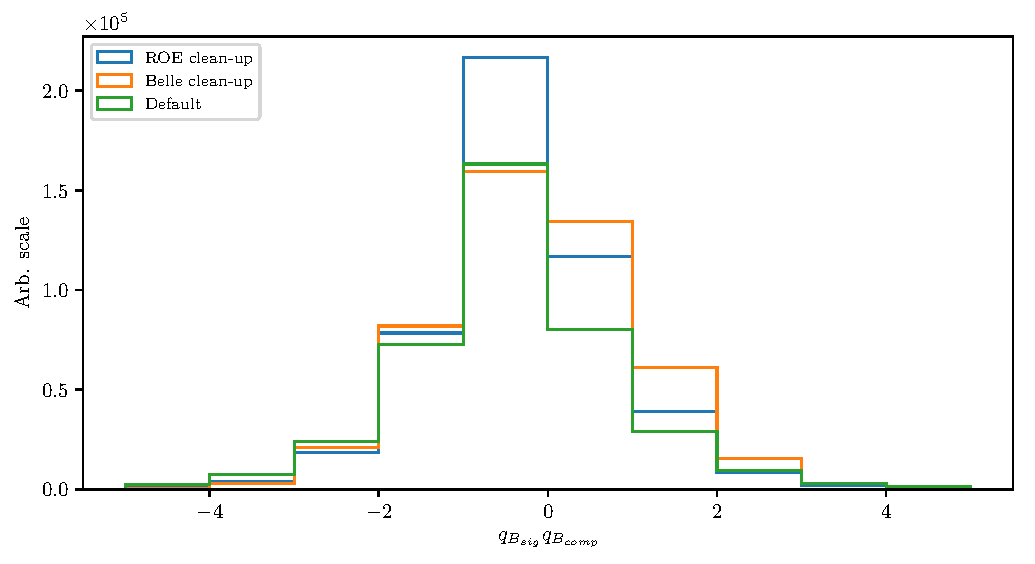
\includegraphics[width=\linewidth]{fig/roe_chargeprod}
\caption{Distribution of $B_{sig}$ and $B_{comp}$ charge product for various types of clean-up procedures. Fore ROE clean-up, the procedure seems to increase the number of candidates with the correct value of the product.}
\label{fig:roe_chargeproduct}
\end{figure}

\begin{figure}[H]
\centering
\captionsetup{width=0.8\linewidth}
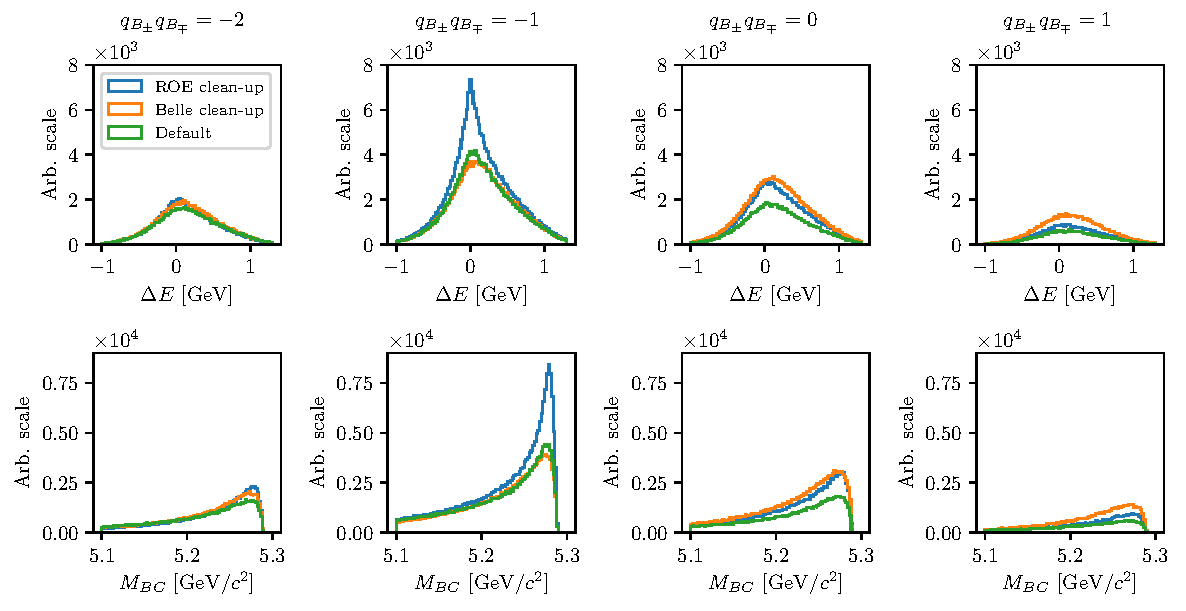
\includegraphics[width=\linewidth]{fig/roe_split}
\caption{Distributions of $\Delta E$ (top) and $M_{BC}$ (bottom)for various types of clean-up procedures, split by specific values of the charge product. While there seems to be an increase in efficiency for both clean-up procedures in general, ROE-cleanup makes the most improvement to resolution and efficiency for the correct value of the charge product.}
\label{fig:roe_split}
\end{figure}

\section{ROE clean-up validation}

The ROE clean-up seems to perform well, but we have to keep in mind that we are testing the procedure on simulated, not real data. Therefore we have to make sure that this procedure performs on simulated as well as real data in the same manner.

Will add more later.

\chapter{Background suppression}\label{sec:background-suppression}

This chapter shows the procedure in suppressing various kinds of background by applying cuts on MVA classifier outputs. 

\section{Control decay and other resonant background}

In this analysis we study decays with kaons in the final state. This means that standard procedures in $b \to u$ analyses in order to suppress $b \to c$ backgrounds, such as $K$-veto, are not possible. As a consequence, our final sample consists of combinations of $K$ pairs coming from $b \to c$  sources, such as $D^0 \to K^+ K^-$. Such candidates usually have resonance-like properties in the two-kaon invariant mass spectrum. Figure \ref{fig:res_bkg} shows this invariant mass spectrum of two kaons, $m_{KK}$, where obvious resonant structures are present from sources like
\begin{itemize}
\item $\phi \to K^+K^-$ (sharp resonance at $\sim1.019\e{GeV}/c^2$),
\item $D^0 \to K^+K^-$ (sharp peak at $\sim 1.864\e{GeV}/c^2$),
\item $D^0 \to K^+ \pi^-$ (wide, shifted peak, due to kaon miss-identification).
\end{itemize}

An opportunity for a control decay choice presents itself as $$B^+ \to D^0 \ell^+ \nu, \quad D^0 \to K^+ K^-,$$ which has very similar properties as the studied signal decay, is much more abundant, and, most importantly, is easy to suppress, since it only populates a very narrow region in the $m_{KK}$ invariant mass spectrum. In order to suppress these resonant backgrounds while studying the signal or control decay, we impose a set of the following cuts

\begin{itemize}
\item Signal decay: $\vert m_{KK} - m_{\phi} \vert > \Delta_\phi$, $\vert m_{KK} - m_{D^0} \vert > \Delta_{D^0}$, $\vert m_{K\pi} - m_{D^0} \vert > \Delta_{D^0}$,
\item Control decay: $\vert m_{KK} - m_{\phi} \vert > \Delta_\phi$, $\vert m_{KK} - m_{D^0} \vert \leq \Delta_{D^0}$, $\vert m_{K\pi} - m_{D^0} \vert > \Delta_{D^0}$,
\end{itemize}

where $m_\phi \approx 1.019\e{GeV}/c^2$ and $m_{D^0} \approx 1.864\e{GeV}/c^2$ are nominal masses of the $\phi$ and $D^0$ mesons, and $\Delta_\phi \approx 8\E{-3}\e{GeV}/c^2$ and $\Delta_{D^0} \approx 1.2\E{-2}\e{GeV}/c^2$ are symmetric cut widths around the nominal mass values for the $\phi$ and $D^0$ mesons, respectively.

\begin{figure}[H]
\centering
\captionsetup{width=0.8\linewidth}
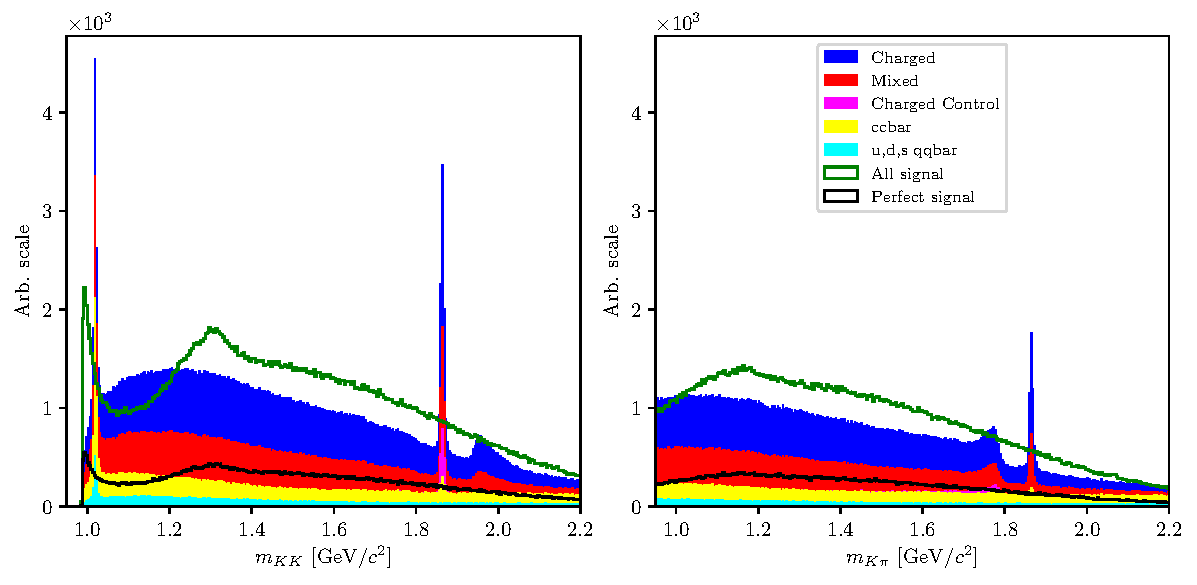
\includegraphics[width=\linewidth]{fig/res_bkg}
\caption{Invariant mass of two correctly reconstructed kaons (left) and invariant mass of two kaons, where one was miss-identified as a pion (right).}
\label{fig:res_bkg}
\end{figure}


\section{Continuum suppression}

Continuum background are physics processes where continuum states are produced in electron and positron collisions $$e^+ e^- \to q \bar q,$$ 
where $q = u,~d,~s$ or $c$, and are a sizable contribution to $B \bar B$ events. Additionally to kinematic constraints to separate $e^+ e^- \to \Upsilon(4S) \to B \bar B$ decays from $e^+ e^- \to q \bar q$, properties of the "event shape" are also often used, because phase-space distributions of decayed particles differ for these two processes. Continuum background events are generated in a back-to-back way in the CMS frame, so hadrons produced in the quark fragmentation possess only a small transverse momentum compared to the initial momentum magnitude. This leads to a spatially confined, jet-like structure. On the other hand $B$ mesons from $B \bar B$ events are produced almost at rest in the CMS frame. Their decay products from an isotropic distribution in the detector, which yields a spherical event shape.

\subsection{Characteristic variables}
\label{ss:charvar}
Information on the phase-space distribution of decay particles is obtained in a number of different ways. In this subsection different characteristic variables are presented which are used in the MVA training. They all focus on kinematic and shape differences between the two processes, which we want to discriminate. 

%\subsubsection{$B$ meson direction}
%Two $B$ mesons, coming from a spin-1 $\Upsilon(4S)$ meson, both have 0 spin, which results in a $\sin^2\theta_B$ angular distribution of the $B$ meson direction with respect to the beam axis. On the other hand, $q \bar q$ final states are represented by two half-spin fermions, which results in two jets, following a $1+\cos^2\theta_B$ distribution. The variable $\vert \cos \theta_B \vert$ allows one to discriminate between $B$ candidates from $B \bar B$ decays and continuum background. Figure X shows the distribution of $\vert \cos \theta_B \vert$ for different $B$ meson candidates.

\subsubsection{Thrust and related variables}
It is possible to define a thrust axis $\mathbf{T}$ for a collection of $N$ momenta $p_i$ as a unit vector along which their total projection is maximal. Thrust axis $\mathbf T$ can be obtained by maximizing the expression
\begin{equation}
\mathbf{T} = \frac{\sum_{i}\vert \mathbf{T} \cdot \mathbf{p}_i\vert}{\sum_{i}\vert \mathbf{p}_i\vert}.
\end{equation}
In this case, a related variable is $\vert \cos\theta_T\vert$, where $\theta_T$ is the angle between the thrust axis of the momenta from $B$ meson decay particles, and the thrust axis of all particles in the ROE. Since both $B$ mesons in $B \bar B$ events are produced at rest, their decay particles, and consequentially their thrust axes, are uniformly distributed in the range $[0,~1]$. On the other hand, decay particles from continuum events follow the direction of the jets in the event. As a consequence, the thrusts of both the $B$ meson and the ROE are strongly directional and collimated, which results in a large peak at $\vert \cos\theta_T\vert \approx 1$. Additionally, one can also use the variable $\vert \cos\theta_{TB}\vert $, which is the thrust axis between the $B$ candidate and the beam axis. For $B$ candidates from $B \bar B$, this distributions is again uniformly distributed, while for candidates from continuum events this distribution follows the distribution of the jets with the function $1+\cos^2\theta_{T,B}$. Figure \ref{fig:cosplots} shows the distributions of $\vert \cos\theta_T\vert$ (left) and $\vert \cos\theta_{T,B}\vert$ (right) for different $B$ meson candidates.

\begin{figure}[H]
\centering
\captionsetup{width=0.8\linewidth}
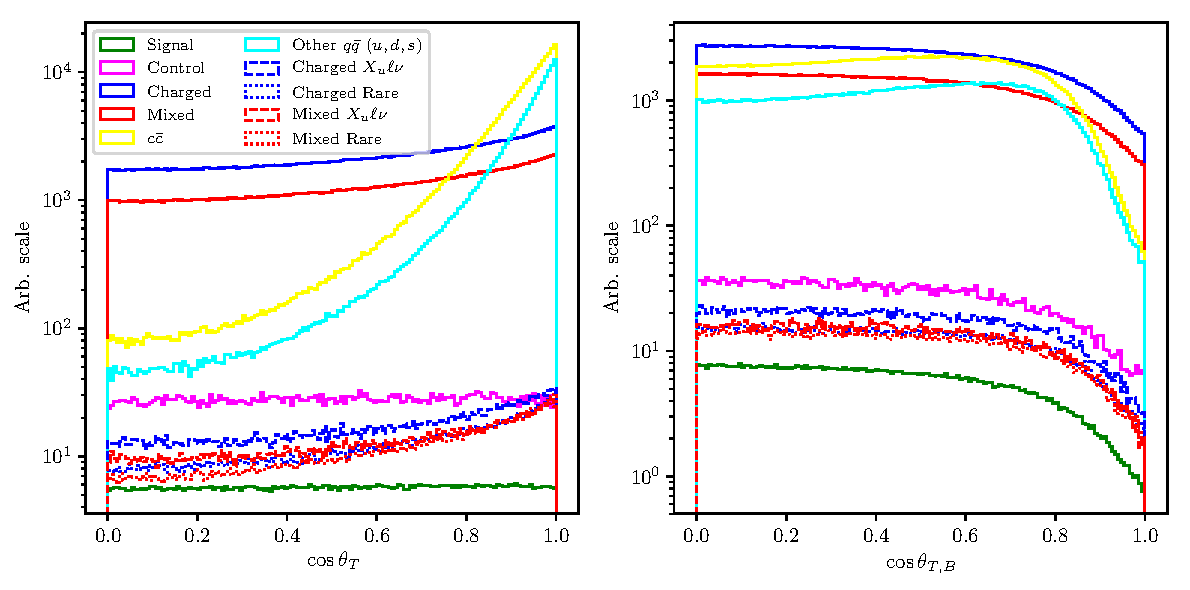
\includegraphics[width=\linewidth]{fig/cs_cosplots}
\caption{Distributions of $\vert \cos\theta_T\vert$ (left) and $\vert \cos\theta_{T,B}\vert$ (right) for different $B$ meson candidates.}
\label{fig:cosplots}
\end{figure}

\subsubsection{CLEO cones}
CLEO cones have been introduced by the CLEO collaboration \cite{asner1996search} and are an additional specific tool to provide optimal background discrimination. They are nine variables corresponding to the momentum flow around the thrust axis of the $B$ meson candidate, binned in nine cones of $10^\circ$ around the thrust axis, as illustrated in Figure \ref{fig:ccones}. 

\begin{figure}[H]
\centering
\captionsetup{width=0.8\linewidth}
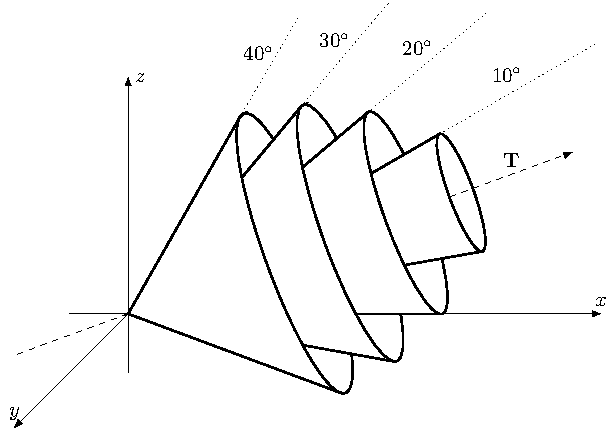
\includegraphics[scale=1]{texfig/CCones}
\caption{Concept of CLEO cones. $\mathbf{T}$ denotes the thrust axis of the $B$ meson candidates in the event. Each variable corresponds to a momentum flow around the thrust axis in steps of $10^\circ$.}
\label{fig:ccones}
\end{figure}

\subsubsection{KSFW moments}
Fox-Wolfram moments are another useful parametrization of phase-space distribution of energy flow and momentum in an event. For a collection of $N$ momenta $p_i$, the $k$-th order normalized Fox-Wolfram moment $R_k$ is defined as
\begin{equation}
R_k = \frac{H_k}{H_0} = \frac{1}{H_0} \sum_{i,j} \vert p_i \vert \vert p_j \vert P_k(\cos \theta_{ij}),
\end{equation}
where $\theta_{ij}$ is the angle between $p_i$ and $p_j$, and $P_k$ is the $k$-th order Legendre polynomial. For events with two strongly collimated jets, $R_k$ takes values close to 0 (1) for odd (even) values of $k$, so these moments provide a convenient discrimination between $B \bar B$ and continuum events.

Belle developed a refined generation of Fox-Wolfram moments, called Kakuno-Super-Fox-Wolfram (KSFW) moments to further suppress the continuum background. There are $17$  different KSFW moments which are grouped into $R^{so}_k$, $R^{oo}_k$ and $R^{ss}_k$ \cite{bevan2014physics}. The latter ones are excluded due to correlations with $B$ meson specific variables.

\subsection{MVA training}
\label{ss:qqmva}
Most of the characteristic variables, described in subsection \ref{ss:charvar}, were taken together in order to train a single MVA classifier for continuum suppression. All characteristic variables were checked for possible $q^2$ correlation. Variables with significant correlation or complex shapes in the 2D plot were discarded from the training set, since they would have introduced unwanted dependence on the unreliable model, ISGW2, used for signal MC generation. Additionally, all of the characteristic variables in our set do not depend on the signal mode, they only differ in the kinematic and topological aspects of $B \bar B$ and continuum background events.

The training dataset consisted of $2\E5$ candidates, where $50~\%$ of the candidates are correctly reconstructed signal events, $25~\%$ are $u \bar u$, $d \bar d$ and $s \bar s$ background with expected proportions, and $25~\%$ is $c \bar c$ background. Since the full Belle dataset is experiment dependent, we construct the training dataset by proportionally sampling each MC dataset, corresponding to the appropriate experiment number.

The training variable set consisted of
\begin{itemize}
\item $B$ meson direction and thrust related variables
	\begin{itemize}
	\item magnitude of thrust axes of $B$ and $ROE$,
	\item cosine of angle between thrust axis of $B$ and thrust axis of ROE,
	\item cosine of angle between thrust axis of $B$ and beam direction,
	\item reduced Fox-Wolfram moment $R_2$	,
	\end{itemize}
\item all $9$ CLEO Cones
\item KSFW Moments
	\begin{itemize}
	\item $R^{so}_{01}$, $R^{so}_{02}$, $R^{so}_{03}$, $R^{so}_{04}$,
	\item $R^{so}_{10}$, $R^{so}_{12}$, $R^{so}_{14}$,
	\item $R^{so}_{20}$, $R^{so}_{22}$, $R^{so}_{24}$,
	\item $R^{oo}_{0}$, $R^{oo}_{1}$, $R^{oo}_{2}$, $R^{oo}_{3}$, $R^{oo}_{4}$,
	\end{itemize}
\item FlavorTagging variables
	\begin{itemize}
	\item $qp$ of $e,~\mu,~\ell$,
    \item $qp$ of intermediate $e,~\mu,~\ell$,
	\item $qp$ of $K$, $K/\pi$, slow pion, fast hadron,
	\item $qp$ of maximum $P^*$, $\Lambda$, fast-slow-correlated (FSC),
	\end{itemize}
\item Other
	\begin{itemize}
	\item $\Delta z$, $\Delta t$.
	\end{itemize}
\end{itemize}

Figure \ref{fig:cs_mva} shows the classifier output for various types of background, all in expected MC proportions. $B$ meson candidates from continuum background are dominant at lower values, while candidates from $B \bar B$ events populate the region with higher values.

\begin{figure}[H]
\centering
\captionsetup{width=0.8\linewidth}
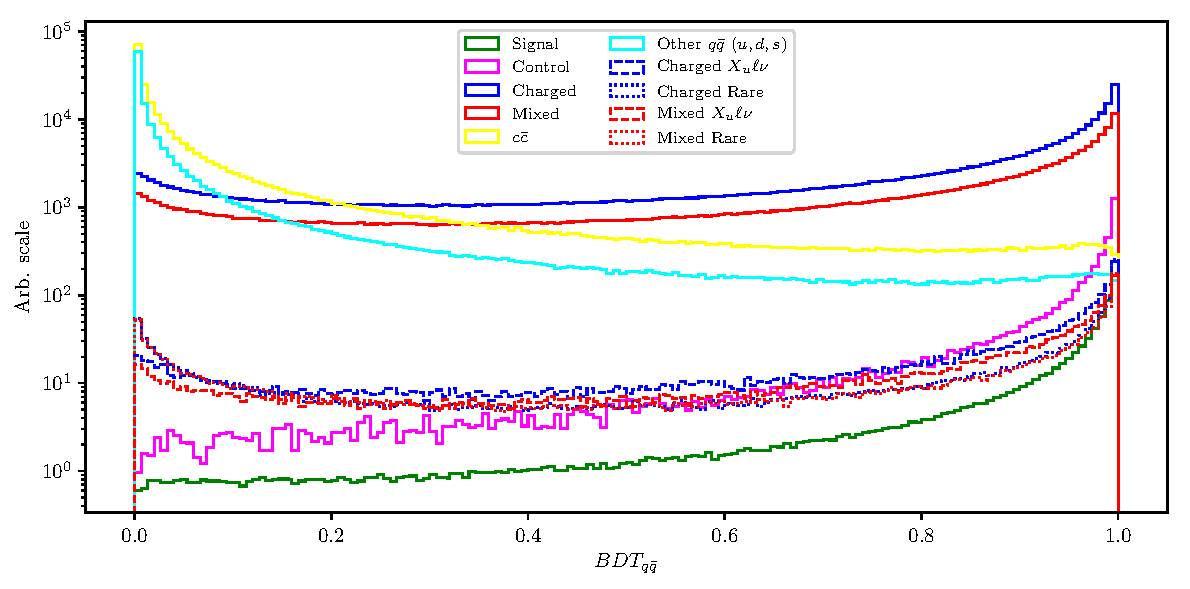
\includegraphics[width=\linewidth]{fig/cs_BDT}
\caption{Continuum suppression classifier output for signal and various types of background. $B$ candidates from continuum events dominate the lower region, while candidates from $B\bar B$ dominate in the upper region of the classifier output.}
\label{fig:cs_mva}
\end{figure}

\section{$B\bar B$ suppression}

After separating continuum background from $B \bar B$ events, the next step is to train an MVA classifier to recognize our signal candidates amongst the candidates of other $B \bar B$ background. $B \bar B$ background consists of
\begin{itemize}
\item $b \to c \ell \nu$ background,
\item $b \to u \ell \nu$ background,
\item Other rare decays (radiative, penguin, rare 2- and 3-body decays, \dots).
\end{itemize}

Similarly as before, the training dataset for this classifier consisted of $2\E5$ candidates, where $50~\%$ of the candidates are correctly reconstructed signal events. The remaining part of the training dataset consists of all background, not including the control sample, because we are not interested in suppressing it directly. The background part of the dataset consists of $75~\%$ charged and neutral $B \bar B$ events in equal proportions, whereas the remaining $25~\%$ is equally populated with charged and neutral $B \bar B$ events from $b \to u \ell \nu$ and other rare decays. The training dataset was proportionally sampled in the same manner as described in subsection \ref{ss:qqmva}.

In order to separate this kind of background, we must be careful not to introduce correlations with the fit variables ($\Delta E$, $M_{BC}$) or any kind of model dependence (correlation with $q^2$). This means that we can not use any information of the decay particles or the candidate, which is of kinematics nature, such as decay particles momenta, decay angles or other variables with such behavior.

The training variable set consisted of
\begin{itemize}
\item fit probability of $P(\chi^2,DOF)$ of the signal candidate and the ROE side, separately,
\item $\cos\theta_{BY}$ from Eq. (\ref{eq:cosby}),
\item $\cos$ of the angle between momentum and vertex of $X$, where $X \in [KK,~KK\ell,~KK\ell\nu]$,
\item FlavorTagger variables for the two signal-side kaons,
\item number of kaons, tracks and distant tracks in ROE,
\item $\theta$ angle of the ROE momentum in CMS frame,
\item $\xi_Z$ from \cite{PhysRevD.83.032007}
\item $\Delta z$,
\item $m_{miss}^2$ from Eq. (\ref{eq:m2def}),
\item $B \to D^* \ell \nu$ veto variables,
\end{itemize}
where distant tracks are all tracks in ROE which satisfy the condition of $\vert d_0 \vert  > 10.0\e{cm}$ or $\vert z_0 \vert > 20.0\e{cm}$. The last entry, $B \to D^* \ell \nu$ veto variables, are a set of variables where we partially reconstruct the $D^*$ candidate 4-momentum via a linear combination of the $\pi^\pm_s$ 4-momentum in the $D^* \to D \pi_s^\pm$ decay. It helps discard the most dominant $B \to D^* \ell \nu$ background. It is most efficient in the $B^0 \to D^{*-} \ell^+ \nu$ decay, where $D^{*-}$ further decays via $D^{*-} \to \bar D {}^0 \pi^-_s$. Other decays do not contain a charged $\pi_s$ particle and are harder to reconstruct with good precision. This results in larger suppression of the neutral $B \bar B$ background only. Figures \ref{fig:vetoplot} shows the veto variable with a partial reconstruction of a charged $\pi_s^\pm$.

\begin{figure}[H]
\centering
\captionsetup{width=0.8\linewidth}
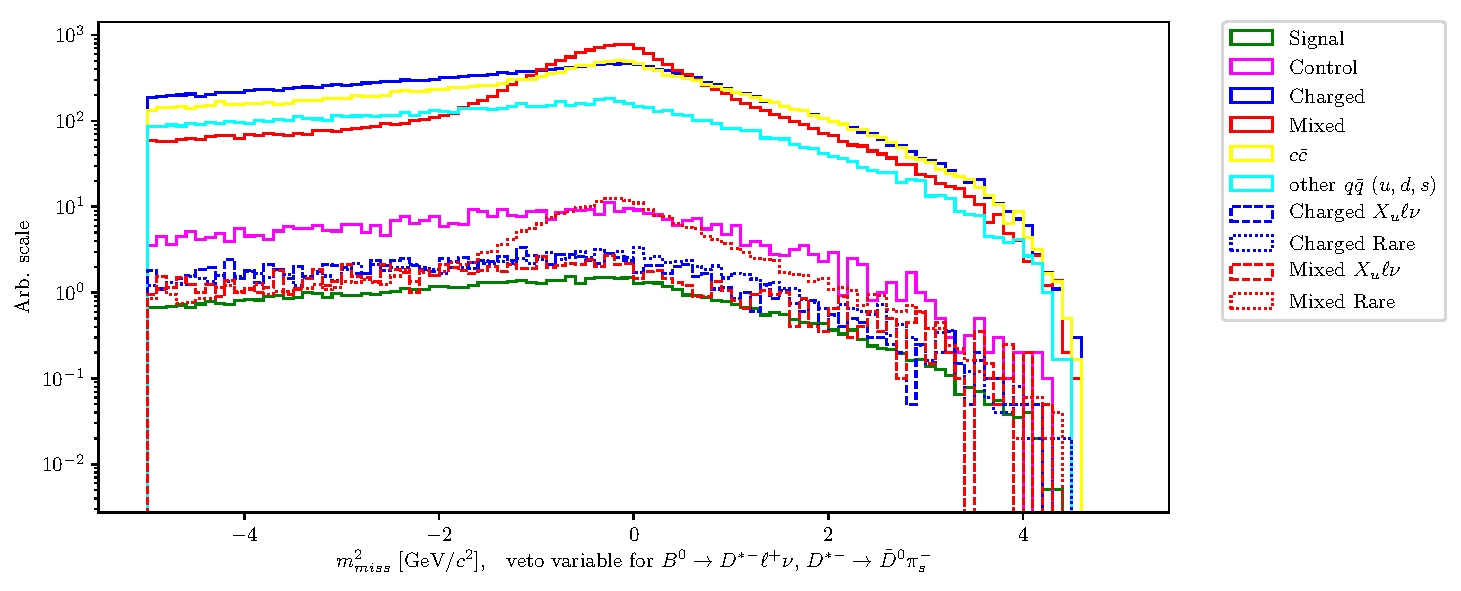
\includegraphics[width=\linewidth]{fig/bb_partial_veto}
\caption{Distribution of $m_{miss}^2$ for partially reconstructed $B^0 \to D^{*-} \ell^+ \nu$ decays, which serves as a veto.}
\label{fig:vetoplot}
\end{figure}

When the training is finished and hyper-parameters of the classifier are optimized, the classifier output, shown in Figure \ref{fig:bbmva} (left), can be used for background suppression. $B$ meson candidates from $B \bar B$ background are dominant at lower values, while candidates from $B \bar B$ events populate the region with higher values. Since the differences between signal and background $B \bar B$ events are smaller than $B \bar B$ and $q \bar q$ events, the resulting classifier has a smaller separation power than in previous section.

\subsection{Boosting to uniformity}
The selection approach with standard classifiers is optimal for counting experiments, as it by construction produces the optimal selection for observing an excess of signal over background events. Today's BDT algorithms, which work in this way, produce non-uniform selection efficiencies and may, as a consequence, shape background distributions to look like signal. In order to minimize such behavior, it is possible to discard variables, which are correlated with the variable of interest (in our case \vars), from the training set. This, however, decreases the classifiers discriminating power. Another approach is to use a novel boosting method, uBoost, which is trained to optimize an integrated FOM under the constraint that the BDT selection efficiency for the desired class must be uniform. The uBoost algorithm balances the biases to produce the optimal uniform selection \cite{stevens2013uboost}.

The training set used in this training is the same as described in the beginning of this chapter, along with the same set of training variables. It will be seen later that the standard BDT classifier shapes the background to look like signal mostly in the $M_{BC}$ picture, therefore we train the uBDT classifier with a uniformity constraint in the $M_{BC}$ variable for background candidates with the uBoost algorithm. The resulting classifier output is shown in Figure \ref{fig:bbmva} (right). For this classifier, the separation power between signal and background seems worse, however, the shapes of backgrounds can differ and the final conclusion will be shown only after the signal extraction.

\begin{figure}[H]
\centering
\captionsetup{width=0.8\linewidth}
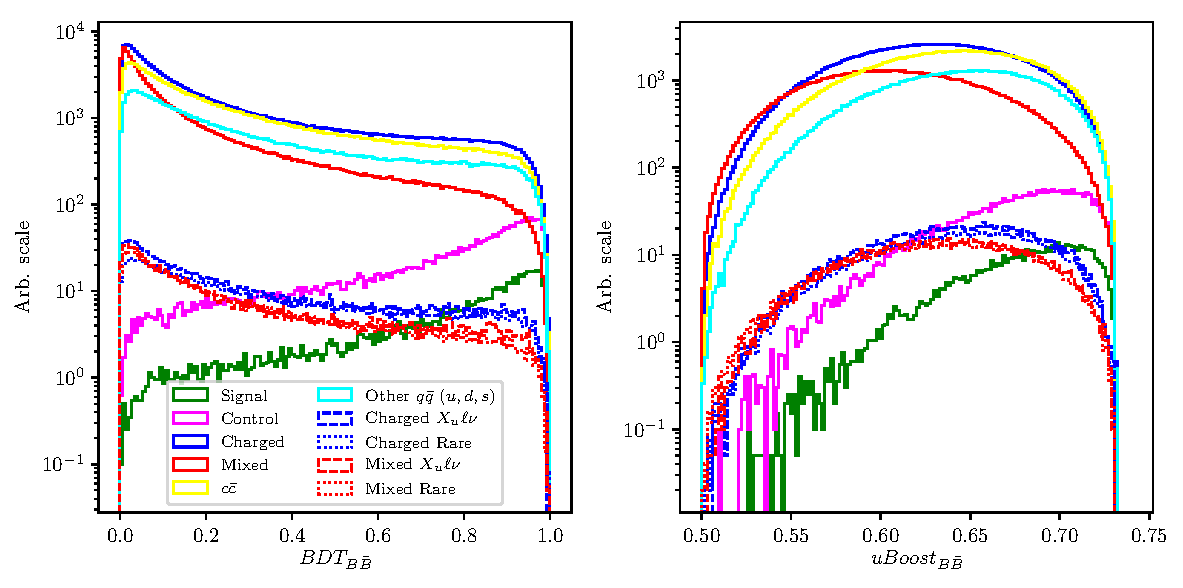
\includegraphics[width=\linewidth]{fig/bb_BDT}
\caption{$B\bar B$ suppression classifier output for signal and various types of background for the standard BDT classifier (left) and the uBDT classifier (right). $B$ candidates from $B\bar B$ background events dominate the lower region, while signal and control candidates dominate in the upper region of the classifier output.}
\label{fig:bbmva}
\end{figure}

\section{Selection optimization}

Instead of two separate $q \bar q$ and $B \bar B$ $FOM$ optimizations, it is more efficient to do a simultaneous 2D $FOM$ optimization, since the two classifiers are not completely uncorrelated. In the same manner as before, $FOM$ is optimized for perfectly reconstructed signal candidates in the signal window, after all the pre-cuts, signal categorization, and after cutting out the background resonances and the control decay. The $FOM$ plot with the optimal point for both $B \bar B$ MVA classifiers is shown in Figure \ref{fig:mvafom}.

\begin{figure}[H]
\centering
\captionsetup{width=0.8\linewidth}
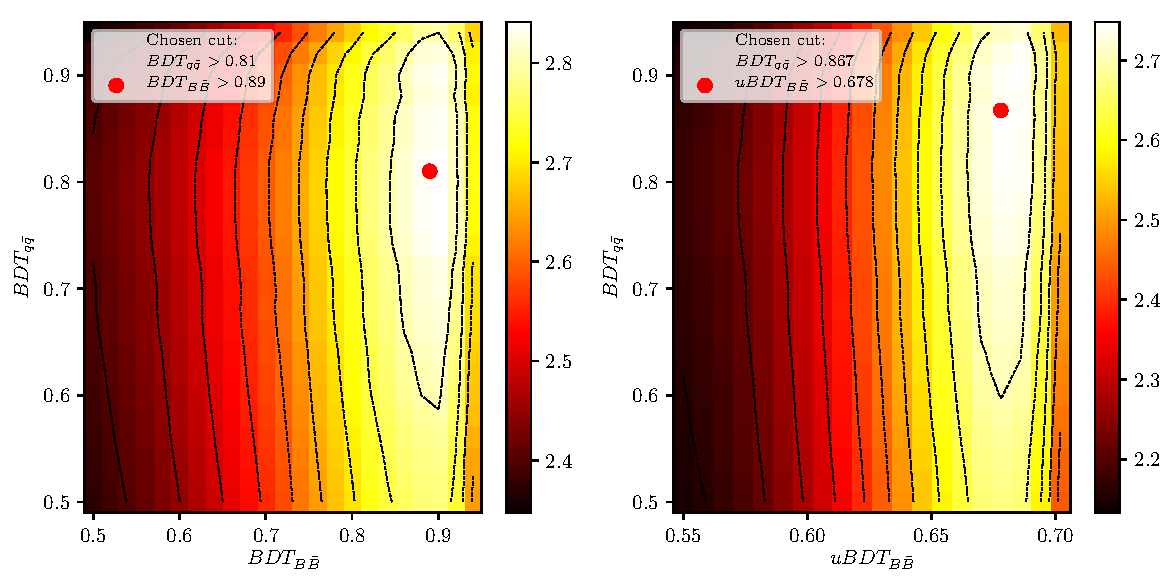
\includegraphics[width=\linewidth]{fig/mva_fom}
\caption{2D $FOM$ optimization of continuum suppression classifier and the standard BDT (left) and uBDT (right) $B\bar B$ suppression classifier.}
\label{fig:mvafom}
\end{figure}

We can compare signal and major background distributions of \vars~after the 2D $FOM$ optimization for both classifiers. Figure \ref{fig:opt01c} shows the arbitrary (left) and normalized scale (right) for $\Delta E$ (top) and $M_{BC}$ (bottom) for the final sample optimized with the standard BDT classifier, while Figure \ref{fig:opt1dc} shows similarly for the final sample optimized with uBDT classifier. We can see that there is considerably more background in the latter case, however, also shapes of background and signal distributions differ greatly. The biggest change seems to be in the shape of the $M_{BC}$ distribution, where the background component is much more signal like in the final sample optimized with the standard BDT classifier than in the other case. The total numbers of expected signal candidates and the signal-to-noise ratios for both classifiers are:
\begin{itemize}
\item Standard BDT: $N_{sig} = 152.82,\quad N_{sig}/N_{bkg} = 3.70~\%$,
\item uBDT: $N_{sig} = 241.56,\quad N_{sig}/N_{bkg} = 1.09~\%$.
\end{itemize}
%TODO: update numbers

\begin{figure}[H]
\centering
\captionsetup{width=0.8\linewidth}
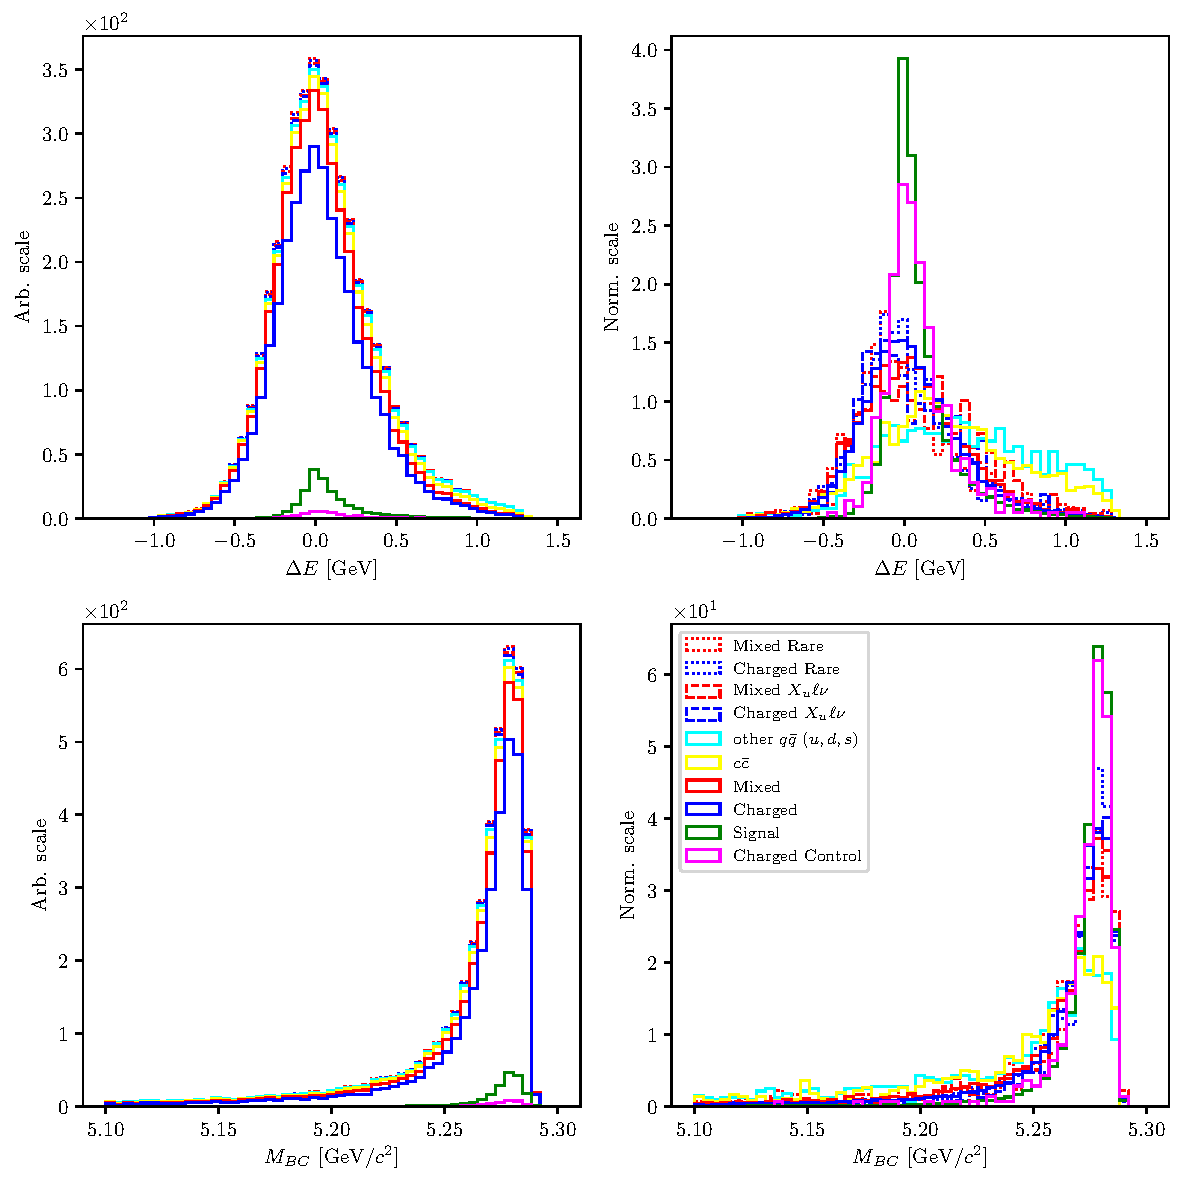
\includegraphics[width=\linewidth]{fig/opt_01c}
\caption{Arbitrary (left) and normalized scale (right) for $\Delta E$ (top) and $M_{BC}$ (bottom) for the final sample optimized with the standard BDT classifier.}
\label{fig:opt01c}
\end{figure} 

\begin{figure}[H]
\centering
\captionsetup{width=0.8\linewidth}
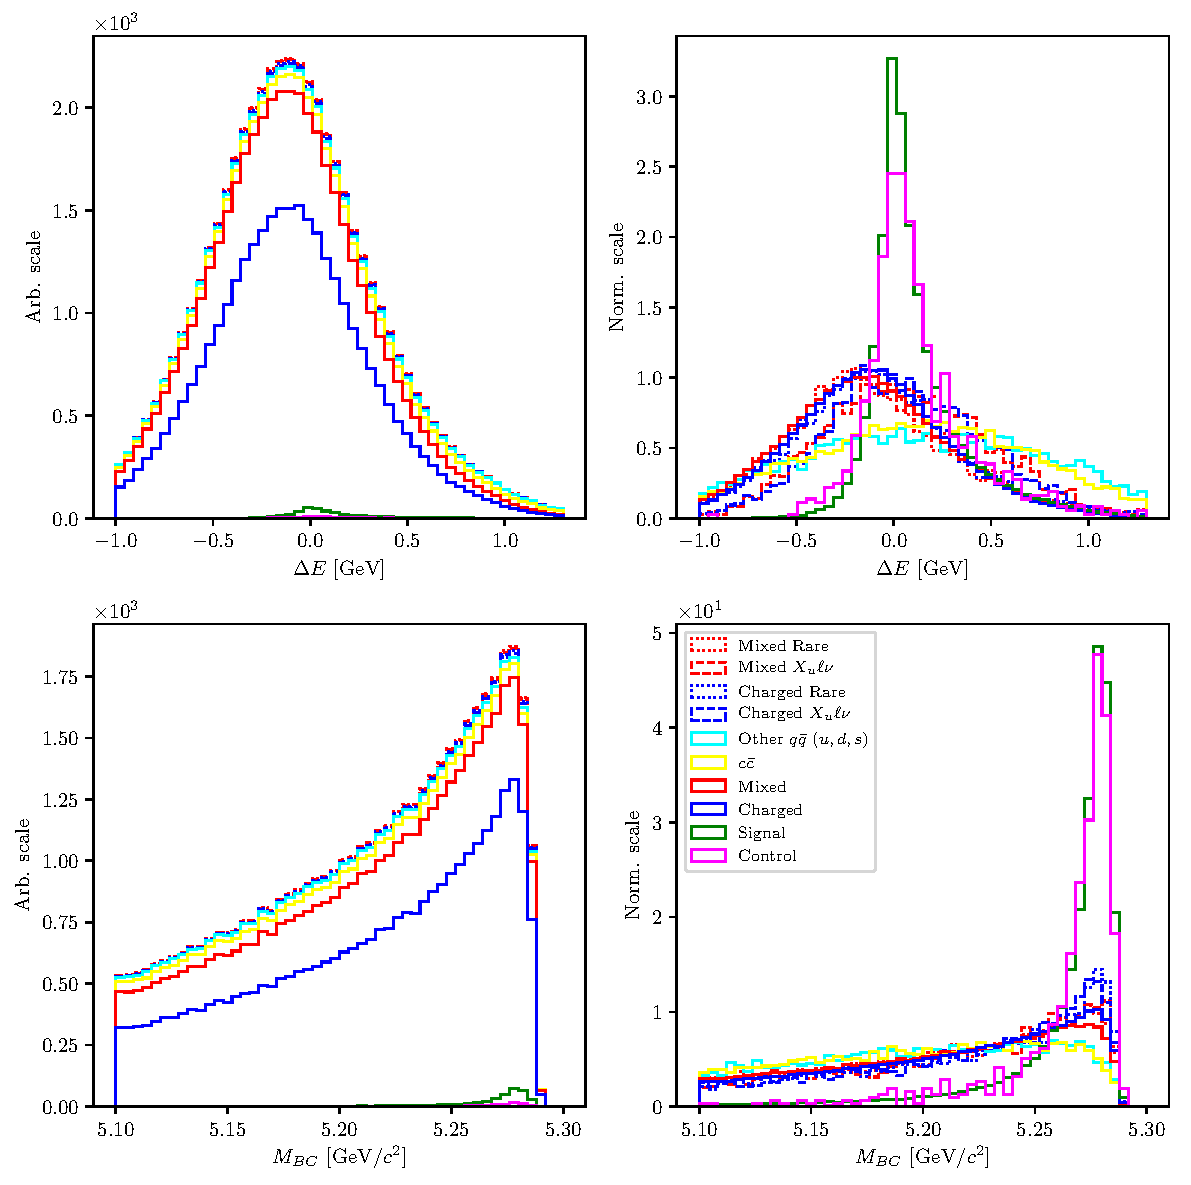
\includegraphics[width=\linewidth]{fig/opt_1dc}
\caption{Arbitrary (left) and normalized scale (right) for $\Delta E$ (top) and $M_{BC}$ (bottom) for the final sample optimized with the uBDT classifier.}
\label{fig:opt1dc}
\end{figure} 

\section{Data and MC agreement}

With the final selection in place, we can check the data and MC agreement by checking the control decay region in on- and off- resonance data. Off-resonance samples provide the ability to check the agreement of the $q\bar q$ background component, while on-resonance samples can be used to check the validity of the control MC sample and, consequentially, the signal MC sample.

The off-resonance data were collected at $60\e{MeV}$ below the $\Upsilon(4S)$ resonance peak energy in order to determine the non-$B\bar B$ background. It therefore offers a direct view of the $q\bar q$ background data sample, which we can compare to the off-resonance MC sample. Figure \ref{fig:offres_control} shows $\Delta E$, $M_{BC}$ and the $q \bar q$ classifier output, $BDT_{q\bar q}$, for off-resonance data and MC in the control region, before any MVA cuts, where the MC sample was scaled down by a factor of $6$, due to having more streams of MC. Figures show a slight and a consistent under-estimation of the $q\bar q$ MC sample. However, looking at the shapes of the fit distributions, the only difference seems to be the normalization factor, so the distribution shapes can be left as they are, since the normalization will be automatically set in the template fit. There also seems to be a difference in the classifier performance for the continuum background suppression on data and MC. This leads to further differences between data and MC in the $q \bar q$ sample after the classifier cut, but we estimate that these differences are negligible, since a relatively small amount of continuum background passes the selection, compared to other background types.

\begin{figure}[H]
\centering
\captionsetup{width=0.8\linewidth}
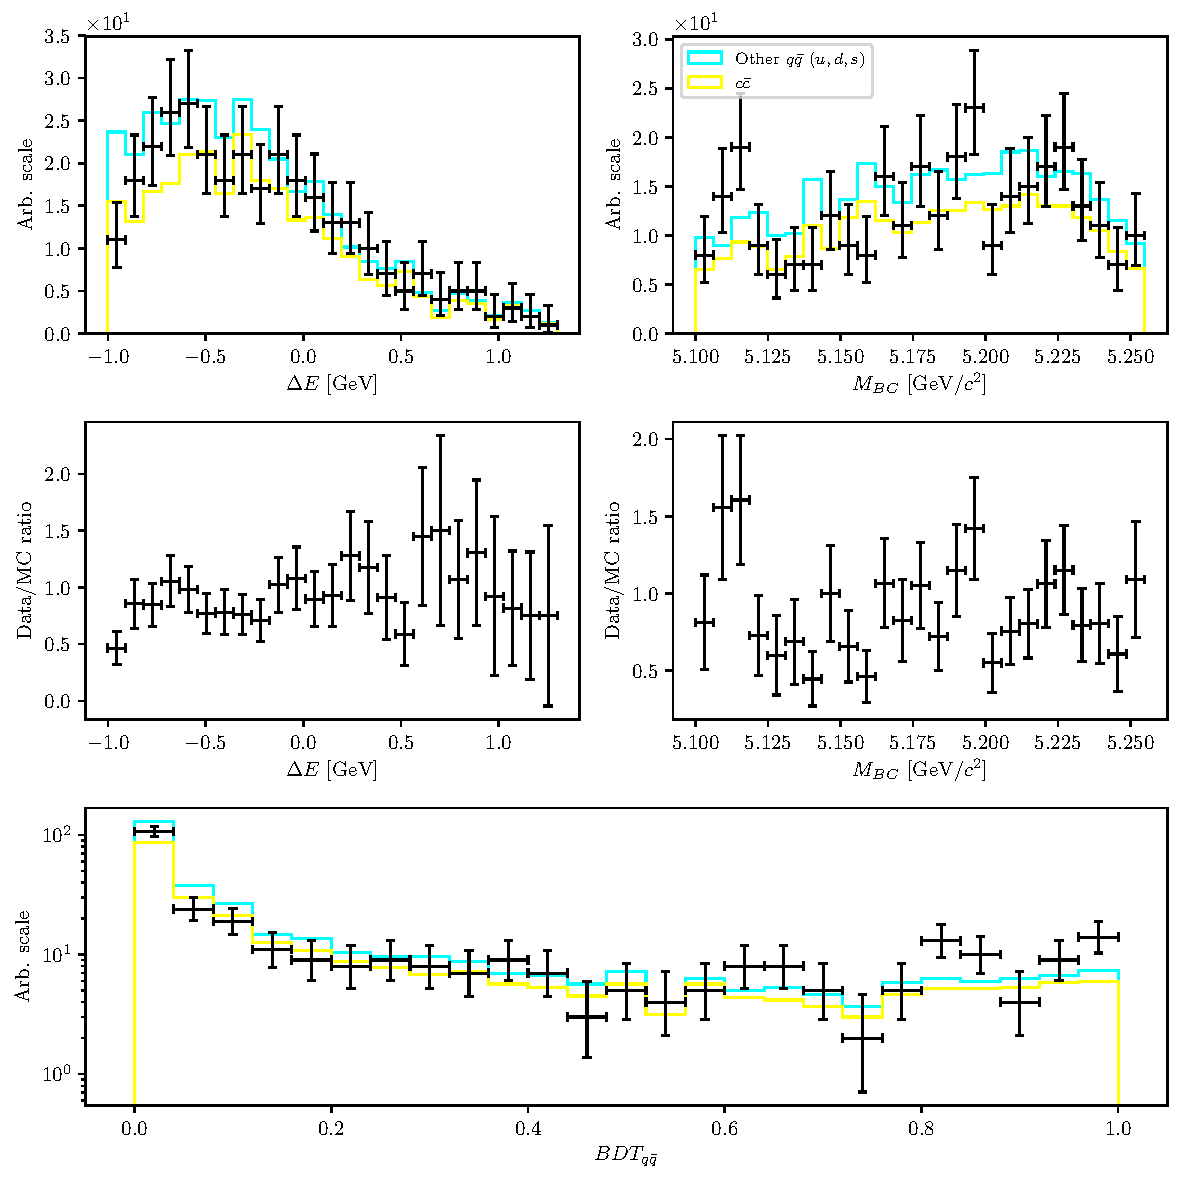
\includegraphics[width=\linewidth]{fig/offres_control}
\caption{$\Delta E$ (left), $M_{BC}$ (right) and the $q \bar q$ classifier output (bottom), for off-resonance data and MC in the control region before any MVA cuts.}
\label{fig:offres_control}
\end{figure}

%ratios of MC and data for these variables before and after the $q\bar q$ MVA cut, shown in Figure X, one can conclude that, based on the flatness of the function,
%PLOT

We can repeat the check on on-resonance data. Figure \ref{fig:onres_control} shows $\Delta E$, $M_{BC}$ and $BDT_{q \bar q}$, where one can see inconsistencies between data and MC on the lower spectrum, where continuum background is dominant. We see that MC is over-estimated in this region, most likely due to additional disagreements from other sources. On the other hand, data and MC seem to agree well in the upper part of the spectrum, where $B \bar B$ events are dominant. Overall, data and MC seem to agree well already off-the-shelf after all the pre-cuts and without any corrections. This means that the modeling of this MC sample is very precise in this particular region of data and that there are no significant differences between data an MC for the control sample and the signal sample.

\begin{figure}[H]
\centering
\captionsetup{width=0.8\linewidth}
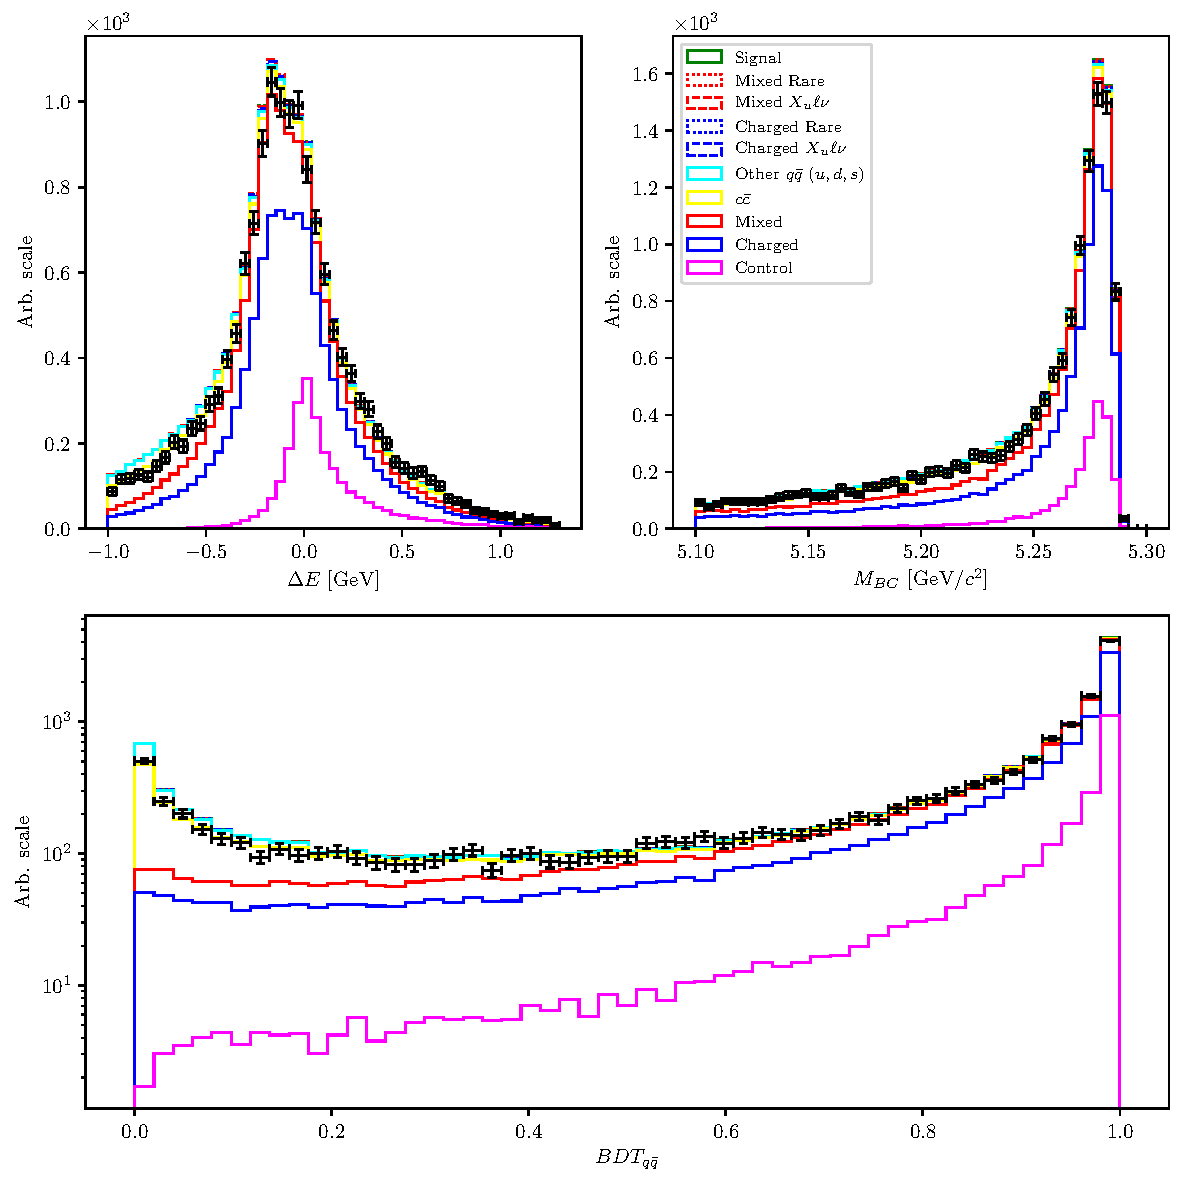
\includegraphics[width=\linewidth]{fig/onres_control}
\caption{$\Delta E$ (left), $M_{BC}$ (right) and the $q \bar q$ classifier output (bottom), for on-resonance data and MC in the control region before any MVA cuts.}
\label{fig:onres_control}
\end{figure}

\chapter{Signal extraction}
In this chapter the procedure for signal yield extraction is presented. We use the framework of \texttt{RooFit} \cite{verkerke2006roofit} where we define 2D histogram templates in \vars, based on MC, for signal and several types of background. Using these templates, the independent full sample is fitted with binned extended maximum likelihood (ML) fit, so that the individual template ratios and their sum describe the fitted sample as best as possible. In particle physics we are often dealing with low numbers of events and need to account for the Poisson nature of the data, therefore we use the likelihood fit, since it takes the Poisson errors into account, unlike the $\chi^2$ fit, where the errors are assumed to be Gaussian. In this procedure we attempt to find the parameter values that maximize the likelihood function, given the observations.

If $P(n\vert\vec \alpha)$ is the probability of measuring $n$ on a given event, where $\vec \alpha$ is a set of parameters on which $P$ depends, we can define the likelihood function $L$ for a series of such measurements (i.e., bins in histogram) $n_i$ based on Poisson statistics as
\begin{equation}
\label{eq:ML}
L(\vec \alpha) = \prod_{i=1} P(n_i|\vec \alpha) = \prod_{i=1} \frac{\mu_i^{n_i}\mathrm{e}^{-\mu_i}}{n_i!},
\end{equation}
where $\mu_i$ is the expected and $n_i$ the measured value for each measurement. It is also common to search for the minimum of the negative value of $\ln L$, or negative log-likelihood (NLL), as
\begin{equation}
\label{eq:NLL}
\mathcal{L}(\vec \alpha) = -\ln L(\vec \alpha) = -\sum_{i}\ln \left(\frac{\mu_i^{n_i}\mathrm{e}^{-\mu_i}}{n_i!}\right) = \sum_{i}\ln(n_i!) + \mu_i - n_i\ln(\mu_i).
\end{equation}
Maximizing $L$ or minimizing $\mathcal{L}$ gives us a maximum likelihood estimate of the set of parameters $\vec \alpha_{ML}$ which best describe the observed data. 

The ML method provides a method to estimate the fit uncertainty. This is especially useful if the log-likelihood has a non-parabolic shape, which leads to asymmetric errors. We calculate the errors using the \texttt{MINOS} algorithm from the \texttt{MINUIT} package \cite{James:1994vla}, which is implemented in RooFit. The algorithm follows the log-likelihood function out of the minimum to find the appropriate intervals of confidence for each parameter, taking the parameter correlations into account. 

To estimate the goodness of the likelihood fit, one option is to generate toy MC experiments and obtain the expected log-likelihood distribution. Likelihood fits, however, also offer another way to test the goodness of fit via the likelihood ratio (LR), where we compare the likelihood obtained under the ML parameters $\vec\alpha_{ML}$, to the likelihood obtained under the null hypothesis parameters $\vec\alpha_{H_0}$. This determines how likely the data is under one model than the other. We define the LR test as
\begin{equation}
\label{eq:lr}
\lambda = -2\ln\left(\frac{L(\vec \alpha_{ML})}{L(\vec \alpha_{H_0})}\right) = -2 \left[ \ln L(\vec \alpha_{ML}) - L(\vec \alpha_{H_0})\right] \sim \chi^2_q,
\end{equation}
which asymptotically behaves as the $\chi^2_q$ distribution with $q=m-n$ degrees of freedom, where $m$ and $n$ are degrees of freedom of $L(\vec \alpha_{ML})$ and $L(\vec \alpha_{H_0})$, respectively. In particle physics we usually study a specific decay and try to perform measurements of the signal yield, so the null hypothesis in this case is that we expect to observe no signal. This means that for the null hypothesis we fix the expected signal yield parameter to zero, while leaving the other parameters of $\vec\alpha_{H_0}$ the same as in $\vec\alpha_{ML}$, which results in $n = m-1$ degrees of freedom and in their difference $q = m -n = 1$. For such a simple $LR$ test of a single parameter the LR test then follows the $\chi^2$ distribution with $1$ degree of freedom. In this case we can define the fit significance from the $\chi^2$ value in units of $\sigma$ as
\begin{equation}
\mathrm{Significance} = \sqrt{\lambda} = \sqrt{\chi^2}.
\end{equation}

\section{Fit templates}

The same MC samples are used for template construction as described in Chapter \ref{sec:data-and-monte-carlo-samples}
\begin{itemize}
\item Signal MC,
\item 10 streams of \texttt{charged} and \texttt{mixed} $B \bar B$ background,
\item 6 streams of $c \bar c$ (\texttt{charm}) and other $q \bar q$ (\texttt{uds}) background,
\item \texttt{ulnu} sample, corresponding to $20\times$ integrated luminosity of the full Belle dataset,
\item \texttt{rare} sample, corresponding to $50\times$ integrated luminosity of the full Belle dataset.
\end{itemize}

We perform 10 fits to each stream of MC, where 9 streams were used for the creation of the templates and the remaining stream was used as data. When fitting real data, all available MC was used for creating the templates. The full signal MC sample was used for the signal template definition in case of MC as well as data fits. The signal part of the \texttt{ulnu} sample was not used in template construction, it was only used as a part of the fitted sample. The following histogram templates were defined for the fits
\begin{itemize}
\item signal template,
\item control template,
\item $B \bar B$ template,
\item $q \bar q$ template.
\end{itemize}

When fitting the signal sample, all template shapes were fixed and all template yields were left as floating parameters in the fit, except in the case of control template, where the yield was fixed to the expected MC value, since the sample size was very small and very similar to the signal template. In case of control sample fits, the yield of the control template was left as a floating parameter, while the yield of the signal template was fixed to the expected MC value for the same reasons as mentioned before. Figures \ref{fig:opt01c} and \ref{fig:opt1dc} show \vars~distributions for the signal template for both final samples, where pronounced peaks can be seen at $\Delta E \approx 0\e{GeV}$ and $M_{BC} \approx m_B$.

The remaining three templates for control, $q \bar q$ and $B \bar B$ sample all describe the background part and, with the exception of the control template, tend to be more widely distributed or even shifted from the nominal value. For the $q \bar q$ template the sample of $q \bar q$ background was used, whereas in case of the control and $B \bar B$ templates, they were constructed using $B \bar B$ background, along with the \texttt{rare} and \texttt{ulnu} background samples with expected relative ratios, based on MC. Figures \ref{fig:opt01c} and \ref{fig:opt1dc} show \vars~distributions for the three types of background for the final selection using the standard $BDT$ and the $uBDT$, respectively.

\section{Adaptive binning algorithm}\label{sec:adaptive-binning-algorithm}

The fit templates contain areas of low statistics, which are populated with bins with zero content. This is a direct consequence of having a finite MC sample and represent a liability in ML fits. Due to low statistic in the edge regions, the locations of these empty bins can vary for the templates and the fitted sample. A problem occurs if all templates have an empty bin where the fitted sample does not. In the scope of ML fits, this effectively means that there are entries in bins where the probability of having them is $0$. We will call such bins \textit{problematic}, because in these cases the fit does not converge.

The ideal solution for this problem would be to increase the MC statistics. Since this is not an option, we pursue other solutions, such as decreasing the number of bins. While this solves the problem, the drawback of it is a decrease in the template resolution in densely populated regions, where good resolution is most needed. The optimal solution here seems to be a choice of variable bins, with fine binning in the densely populated regions and larger bins in the regions with low statistics.

We have devised an algorithm, which compares the templates and the fitted sample, and defines a variable binning so that there are no more problematic bins in the end. Figure \ref{fig:adapt} shows an example of how the procedure works. The algorithm takes an argument for the initial number of uniform bins in each dimension, and does the following
\begin{enumerate}
\item define uniform binning in both dimensions with the provided argument,
\item create a 2D histogram from MC templates with expected yields,
\item define an \textit{optimal} region, where most of the 2D integral is contained and where all bins have a non-zero content (this region does not change throughout the process),
\item compare the histograms for the expected and the fitted sample, find the problematic bins,
\item loop until all problematic bins disappear
	\begin{enumerate}
	\item find problematic bin, which is nearest to the maximum bin,
	\item change the binning from $N$ to $N-1$ from that bin and in the direction away from the maximum bin.
	\end{enumerate}
\end{enumerate}

\begin{figure}[H]
	\centering
	\captionsetup{width=0.8\linewidth}
	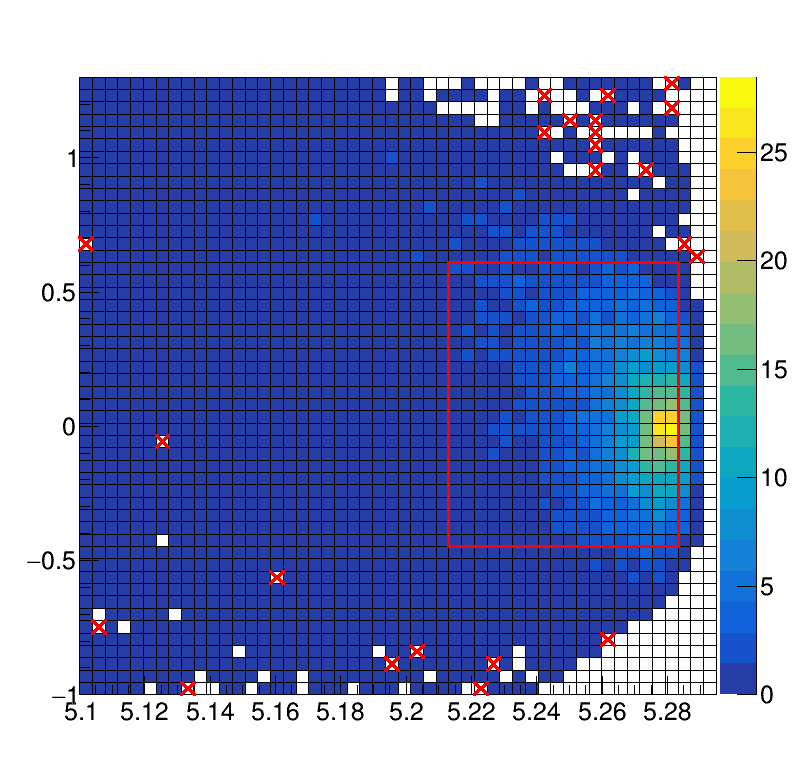
\includegraphics[width=0.49\linewidth]{fig/adaptive_1}
	\includegraphics[width=0.49\linewidth]{fig/adaptive_15}
	\caption{Steps taken in the adaptive binning algorithm. Left image shows the initial 2D histogram with the defined optimal region and the problematic bins, the right image shows the final binning with the unchanged optimal region, while the problematic bins are gone due to the new binning choice.}
	\label{fig:adapt}
\end{figure}

An additional problem seems to be the plotting of the fitted templates and the sample with variable binning. It would seem that RooFit does not take the bin widths into account when plotting, while everything works as expected for the fit itself. This was bypassed by extracting the fitted yields and applying them to templates and samples with uniform binning, which were then used for drawing.

\section{Signal MC fit results}\label{sec:signal-mc-fit-results}

The fit setup was used on the final samples obtained with both versions of the final selection (standard BDT and uBDT). The choice of the initial uniform binning is not obvious, so we perform fits to all streams of MC for each initial binning choice and the fitted and expected yield difference, pulls and fit significance for both final samples, shown in Figure \ref{fig:sig_binning}. Fits to final sample, obtained with the uBDT classifier generally seem to have a lower bias, pull distributions closer to the normal distribution and better significance than the fits in the case of the standard BDT final sample. This fixes our choice of the final selection. It is also possible to determine the optimal initial binning choice to be somewhere in the region of $22$ bins in each dimension, since a higher number of initial bins yields biased results, while a lower one yields results with poorer significance.

\begin{figure}[H]
	\centering
	\captionsetup{width=0.8\linewidth}
	\includegraphics[width=\linewidth]{fig/sig_binning}
	\caption{Fitted yield and expected yield difference (top), pulls (center) and fit significance (bottom) as a function of binning in \vars~for the final sample, optimized with the standard BDT classifier (blue) and the uBDT classifier (orange).}
	\label{fig:sig_binning}
\end{figure}

Figure \ref{fig:sig_streamfit} shows the fit result and the fitted sample of an arbitrary stream for \vars, for the fit region and for the signal region. The fits seem stable and under control. Fit results for all streams of MC are shown in Figure \ref{fig:sig_global}, along with the global fit over all streams. The results seem to describe the expected value in a precise manner, with the bias much smaller than the average statistical error. The normalized $\chi^2$ value with $9$ degrees of freedom of the global fit is $\chi^2_9 = 0.72$, while the average significance of the fits is around $2.75 \sigma$.

\begin{figure}[H]
	\centering
	\captionsetup{width=0.8\linewidth}
	\includegraphics[width=\linewidth]{fig/plt_uMVA1dc_0.png}
	\caption{An example fit to one stream of MC. Left column shows the $M_{BC}$ and the center column shows the $\Delta E$ distribution of the full fitted sample in the full fit region (top) and the signal region (bottom). The right column shows the expected 2D histogram in \vars~with initial uniform binning (top) and the variable binning (bottom) after the binning algorithm.}
	\label{fig:sig_streamfit}
\end{figure}

\begin{figure}[H]
	\centering
	\captionsetup{width=0.8\linewidth}
	\includegraphics[width=\linewidth]{fig/sig_global}
	\caption{Fits to all 10 streams of MC and the global fit with a zero degree polynomial. The red like shows the mean value of the global fit and the green band shows the $1\sigma$ confidence interval.}
	\label{fig:sig_global}
\end{figure}

\subsection{Toy MC experiment}

Toy MC experiments allow us to study the yields, errors and the pulls of the signal fit by generating our own pseudo datasets, according to the MC, and not producing it in the standard way, which consumes unaffordable amounts of CPU time. In order to test the fit behavior, a toy MC study was performed where all available MC was used for template creation. We constructed $3\E{3}$ pseudo datasets, where each dataset was generated expected amount of each template category, distributed according to the Poisson distribution. All fits were performed with the optimal initial uniform binning of $22\times22$ bins in \vars.

Figure \ref{fig:toyMC} shows distributions of the fit yields, errors and the pull distribution of all pseudo fits. The fits seem to be under control since there is not any significant bias, and the pulls follow a normal distribution with a mean of $(-4\pm18)\E{3}$ and standard deviation of $(1.009\pm0.013)$. The mean ($\bar X$) and the standard deviation $(S)$ were calculated in the usual way, while the errors of these statistics were obtained by calculating the standard error of the mean ($\sigma_{\bar X}$) and standard deviation ($\sigma_S$), taken from \cite{ahn2003standard}, as
\begin{equation}
\sigma_{\bar X} = \frac{S}{\sqrt{N}},\quad \sigma_{S} = \frac{S}{\sqrt{2(N-1)}},
\end{equation}
where $N$ is the number of performed measurements.

\begin{figure}[H]
	\centering
	\captionsetup{width=0.8\linewidth}
	\includegraphics[width=\linewidth]{fig/toyMC}
	\caption{Toy MC fits of pseudo data showing the fit yield (top), fit errors (center) and the pull distribution of the fits (bottom).}
	\label{fig:toyMC}
\end{figure}

\subsection{Toy MC linearity test}
Linearity test is used for determining sensitivity of the fit to the amount of signal in the fitted sample. Since this is a first measurement of this decay channel, MC modeling is not reliable and could be very different from reality, so we need to perform this test in order to determine our sensitivity to smaller, as well as larger amounts of expected signal.

The pseudo datasets are generated in the same way as in the previous subsection, with the exception of signal, which is generated with various amounts. $50$ steps from $[0.1,~10]$ in the logarithmic scale are taken for fractions of signal amount and for each fraction we generate 600 pseudo datasets according to Poisson statistics.

Figure \ref{fig:lin_test} shows the mean fit yield and expected yield difference, mean pull and the mean significance at each signal fraction value. The expected MC result is shown at fraction value $1$. The plots show no significant bias with with respect to the signal fraction, while the pulls seems to be described by the normal distributions throughout the fraction range. At expected value we are just below $3\sigma$ significance, as already pointed out at the beginning of this section.

\begin{figure}[H]
	\centering
	\captionsetup{width=0.8\linewidth}
	\includegraphics[width=\linewidth]{fig/lin_test}
	\caption{Mean fit yield and expected yield difference (top), mean pull (center) and mean significance (bottom) as a function of signal fraction.}
	\label{fig:lin_test}
\end{figure}

\section{Control fit results}

The same fit procedure as in Section \ref{sec:signal-mc-fit-results} is applied to the control decay. This enables us to compare the fit behavior on MC as well as data and check the MC/data agreement. The control sample is also used to check the behavior of several MVA classifier cuts on data and MC. We compare control yields, their ratios and ratios of cut efficiencies (double ratios). The following cut scenarios were studied
\begin{itemize}
\item[(a)]  after pre-cuts,\, $\vert m_{miss}^2 \vert < 1.1\e{GeV}/c^2$,\, $q_{B_{sig}}~q_{B_{comp}} = -1$,
\item[(b)] (a) + $BDT_{had.}$ cut (signal category I),
\item[(c)] (b) + $BDT_{q\bar q}$ cut,
\item[(d)] (b) + $uBDT_{B\bar B}$ cut,
\item[(e)] (b) + $BDT_{q\bar q} + uBDT_{B\bar B}$ cut (final selection).
\end{itemize}

The same binning was chosen as in the case of signal MC fits. The results for control fit yields, their ratios and double ratios are shown in Figure \ref{fig:cs_fits}. The plot shows an under-estimation of MC, which seems to be consistent and under control. On the other hand we also see that the cut efficiency ratios between data and MC are consistent with $1$. This means that the inconsistencies between data and MC, which are present since before applying any MVA cuts, are not introduce nor affect by these cuts.

\begin{figure}[H]
	\centering
	\captionsetup{width=0.8\linewidth}
	\includegraphics[width=\linewidth]{fig/cs_fits.pdf}
	\caption{Fit yields, their ratios and ratios of cut efficiencies (double ratios) for the control sample fits to data and MC.}
	\label{fig:cs_fits}
\end{figure}

\subsection{Branching ratio measurement and comparison}

\section{Signal fit to data}

\chapter{Systematics}
\section{Model uncertainty effects}
\section{PID efficiency correction}
\section{Bias}

\printbibliography

\chapter*{A: MVA control plots}
\section*{ROE clean-up $\pi^0$ training}

\subsection*{Variable importance}

\begin{longtable}{| p{.05\textwidth} | p{.6\textwidth} | p{.05\textwidth} |p{.2\textwidth} |}
\hline
& Name & Alias & Importance \\ \hline
0 &\texttt{chiProb} & $v_{0}$ & $0.262$ \\ \hline
1 &\texttt{useCMSFrame(daughterAngleInBetween(0,1))} & $v_{1}$ & $0.148$ \\ \hline
2 &\texttt{daughter(0,useCMSFrame(p))} & $v_{2}$ & $0.079$ \\ \hline
3 &\texttt{InvM} & $v_{3}$ & $0.076$ \\ \hline
4 &\texttt{daughter(1,clusterHighestE)} & $v_{4}$ & $0.062$ \\ \hline
5 &\texttt{daughter(1,p)} & $v_{5}$ & $0.050$ \\ \hline
6 &\texttt{daughter(1,clusterTheta)} & $v_{6}$ & $0.048$ \\ \hline
7 &\texttt{daughter(0,clusterHighestE)} & $v_{7}$ & $0.031$ \\ \hline
8 &\texttt{daughter(0,clusterTheta)} & $v_{8}$ & $0.028$ \\ \hline
9 &\texttt{daughter(0,minC2HDist)} & $v_{9}$ & $0.023$ \\ \hline
10 &\texttt{daughter(1,minC2HDist)} & $v_{10}$ & $0.021$ \\ \hline
11 &\texttt{daughter(0,clusterE9E25)} & $v_{11}$ & $0.021$ \\ \hline
12 &\texttt{daughter(1,clusterE9E25)} & $v_{12}$ & $0.021$ \\ \hline
13 &\texttt{useRestFrame(daughterAngleInBetween(0,1))} & $v_{13}$ & $0.018$ \\ \hline
14 &\texttt{daughter(1,clusterNHits)} & $v_{14}$ & $0.013$ \\ \hline
15 &\texttt{SigMBF} & $v_{15}$ & $0.013$ \\ \hline
16 &\texttt{daughter(0,clusterNHits)} & $v_{16}$ & $0.013$ \\ \hline
17 &\texttt{useCMSFrame(p)} & $v_{17}$ & $0.012$ \\ \hline
18 &\texttt{daughter(0,clusterErrorE)} & $v_{18}$ & $0.011$ \\ \hline
19 &\texttt{useLabFrame(daughterAngleInBetween(0,1))} & $v_{19}$ & $0.010$ \\ \hline
20 &\texttt{daughter(1,clusterErrorE)} & $v_{20}$ & $0.010$ \\ \hline
21 &\texttt{daughter(1,useCMSFrame(p))} & $v_{21}$ & $0.008$ \\ \hline
22 &\texttt{daughter(0,p)} & $v_{22}$ & $0.007$ \\ \hline
23 &\texttt{p} & $v_{23}$ & $0.007$ \\ \hline
24 &\texttt{SigM} & $v_{24}$ & $0.007$ \\ \hline
\captionsetup{width=0.8\linewidth}
\caption{Variable names, aliases and importance in the scope of $\pi^0$ MVA training for ROE clean-up.}
\end{longtable}

\subsection*{Variable distributions}

\begin{figure}[H]
\centering
\captionsetup{width=0.8\linewidth}
\subfigure{\includegraphics[width=0.241\linewidth]{fig/addendums/pi0_v0}}
\subfigure{\includegraphics[width=0.241\linewidth]{fig/addendums/pi0_v1}}
\subfigure{\includegraphics[width=0.241\linewidth]{fig/addendums/pi0_v2}}
\subfigure{\includegraphics[width=0.241\linewidth]{fig/addendums/pi0_v3}}\\
\subfigure{\includegraphics[width=0.241\linewidth]{fig/addendums/pi0_v4}}
\subfigure{\includegraphics[width=0.241\linewidth]{fig/addendums/pi0_v5}}
\subfigure{\includegraphics[width=0.241\linewidth]{fig/addendums/pi0_v6}}
\subfigure{\includegraphics[width=0.241\linewidth]{fig/addendums/pi0_v7}}\\
\subfigure{\includegraphics[width=0.241\linewidth]{fig/addendums/pi0_v8}}
\subfigure{\includegraphics[width=0.241\linewidth]{fig/addendums/pi0_v9}}
\subfigure{\includegraphics[width=0.241\linewidth]{fig/addendums/pi0_v10}}
\subfigure{\includegraphics[width=0.241\linewidth]{fig/addendums/pi0_v11}}\\
\subfigure{\includegraphics[width=0.241\linewidth]{fig/addendums/pi0_v12}}
\subfigure{\includegraphics[width=0.241\linewidth]{fig/addendums/pi0_v13}}
\subfigure{\includegraphics[width=0.241\linewidth]{fig/addendums/pi0_v14}}
\subfigure{\includegraphics[width=0.241\linewidth]{fig/addendums/pi0_v15}}
\caption{Feature distributions for MVA training of $\pi^0$ candidates in the scope of ROE clean-up.}
\end{figure}

\begin{figure}[H]\ContinuedFloat
\captionsetup{width=0.8\linewidth}
\subfigure{\includegraphics[width=0.241\linewidth]{fig/addendums/pi0_v16}}
\subfigure{\includegraphics[width=0.241\linewidth]{fig/addendums/pi0_v17}}
\subfigure{\includegraphics[width=0.241\linewidth]{fig/addendums/pi0_v18}}
\subfigure{\includegraphics[width=0.241\linewidth]{fig/addendums/pi0_v19}}\\
\subfigure{\includegraphics[width=0.241\linewidth]{fig/addendums/pi0_v20}}
\subfigure{\includegraphics[width=0.241\linewidth]{fig/addendums/pi0_v21}}
\subfigure{\includegraphics[width=0.241\linewidth]{fig/addendums/pi0_v22}}
\subfigure{\includegraphics[width=0.241\linewidth]{fig/addendums/pi0_v23}}\\
\subfigure{\includegraphics[width=0.241\linewidth]{fig/addendums/pi0_v24}}
\caption{Feature distributions for MVA training of $\pi^0$ candidates in the scope of ROE clean-up.}
\end{figure}

\subsection*{Hyper-parameter optimization}

\begin{figure}[H]
\centering
\captionsetup{width=0.8\linewidth}
\includegraphics[width=\linewidth]{fig/addendums/pi0_hpo}
\caption{Hyper-parameter optimization of \texttt{nTrees} and \texttt{nLevels} in the BDT forest training of $\pi^0$ candidates in the scope of the ROE clean-up.}
\end{figure}

\subsection*{Results}

\begin{figure}[H]
\centering
\captionsetup{width=0.8\linewidth}
\includegraphics[width=\linewidth]{fig/addendums/pi0_effpur}
\caption{Efficiency ($\mathcal{E}$) and purity ($\mathcal{P}$) of the MVA classifier output for $\pi^0$ candidates training on the train (solid) and test (dashed) samples.}
\end{figure}

\begin{figure}[H]
\centering
\captionsetup{width=0.8\linewidth}
\includegraphics[width=\linewidth]{fig/addendums/pi0_roc}
\caption{ROC curves of the MVA classifier output for $\pi^0$ candidates training on the train (solid) and test (dashed) samples.}
\end{figure}

\section*{ROE clean-up $\gamma$ training}

\subsection*{Variable importance}

\begin{longtable}{| p{.05\textwidth} | p{.6\textwidth} | p{.05\textwidth} |p{.2\textwidth} |}
\hline
& Name & Alias & Importance \\ \hline
0 &\texttt{p} & $v_{0}$ & $0.317$ \\ \hline
1 &\texttt{clusterHighestE} & $v_{1}$ & $0.251$ \\ \hline
2 &\texttt{pi0p} & $v_{2}$ & $0.183$ \\ \hline
3 &\texttt{minC2HDist} & $v_{3}$ & $0.058$ \\ \hline
4 &\texttt{cosTheta} & $v_{4}$ & $0.044$ \\ \hline
5 &\texttt{clusterNHits} & $v_{5}$ & $0.031$ \\ \hline
6 &\texttt{clusterE9E25} & $v_{6}$ & $0.030$ \\ \hline
7 &\texttt{useCMSFrame(p)} & $v_{7}$ & $0.028$ \\ \hline
8 &\texttt{clusterUncorrE} & $v_{8}$ & $0.023$ \\ \hline
9 &\texttt{clusterR} & $v_{9}$ & $0.019$ \\ \hline
10 &\texttt{clusterErrorE} & $v_{10}$ & $0.011$ \\ \hline
11 &\texttt{clusterReg} & $v_{11}$ & $0.006$ \\ \hline
\captionsetup{width=0.8\linewidth}
\caption{Variable names, aliases and importance in the scope of $\gamma$ MVA training for ROE clean-up.}
\end{longtable}

\subsection*{Variable distributions}

\begin{figure}[H]
\centering
\captionsetup{width=0.8\linewidth}
\subfigure{\includegraphics[width=0.241\linewidth]{fig/addendums/gamma_v0}}
\subfigure{\includegraphics[width=0.241\linewidth]{fig/addendums/gamma_v1}}
\subfigure{\includegraphics[width=0.241\linewidth]{fig/addendums/gamma_v2}}
\subfigure{\includegraphics[width=0.241\linewidth]{fig/addendums/gamma_v3}}\\
\subfigure{\includegraphics[width=0.241\linewidth]{fig/addendums/gamma_v4}}
\subfigure{\includegraphics[width=0.241\linewidth]{fig/addendums/gamma_v5}}
\subfigure{\includegraphics[width=0.241\linewidth]{fig/addendums/gamma_v6}}
\subfigure{\includegraphics[width=0.241\linewidth]{fig/addendums/gamma_v7}}\\
\subfigure{\includegraphics[width=0.241\linewidth]{fig/addendums/gamma_v8}}
\subfigure{\includegraphics[width=0.241\linewidth]{fig/addendums/gamma_v9}}
\subfigure{\includegraphics[width=0.241\linewidth]{fig/addendums/gamma_v10}}
\subfigure{\includegraphics[width=0.241\linewidth]{fig/addendums/gamma_v11}}\\
\caption{Feature distributions for MVA training of $\gamma$ candidates in the scope of ROE clean-up.}
\end{figure}

\subsection*{Hyper-parameter optimization}

\begin{figure}[H]
\centering
\captionsetup{width=0.8\linewidth}
\includegraphics[width=\linewidth]{fig/addendums/gamma_hpo}
\caption{Hyper-parameter optimization of \texttt{nTrees} and \texttt{nLevels} in the BDT forest training of $\gamma$ candidates in the scope of the ROE clean-up.}
\end{figure}

\subsection*{Results}

\begin{figure}[H]
\centering
\captionsetup{width=0.8\linewidth}
\includegraphics[width=\linewidth]{fig/addendums/gamma_effpur}
\caption{Efficiency ($\mathcal{E}$) and purity ($\mathcal{P}$) of the MVA classifier output for $\gamma$ candidates training on the train (solid) and test (dashed) samples.}
\end{figure}

\begin{figure}[H]
\centering
\captionsetup{width=0.8\linewidth}
\includegraphics[width=\linewidth]{fig/addendums/gamma_roc}
\caption{ROC curves of the MVA classifier output for $\gamma$ candidates training on the train (solid) and test (dashed) samples.}
\end{figure}

\section*{ROE clean-up duplicate pair training}

\subsection*{Variable importance}

\begin{longtable}{| p{.05\textwidth} | p{.6\textwidth} | p{.05\textwidth} |p{.2\textwidth} |}
\hline
& Name & Alias & Importance \\ \hline
0 &\texttt{useCMSFrame(daughterAngleInBetween(0,1))} & $v_{0}$ & $0.140$ \\ \hline
1 &\texttt{daughter(1,d0Err)} & $v_{1}$ & $0.084$ \\ \hline
2 &\texttt{useLabFrame(daughterAngleInBetween(0,1))} & $v_{2}$ & $0.056$ \\ \hline
3 &\texttt{daughter(1,d0)} & $v_{3}$ & $0.048$ \\ \hline
4 &\texttt{daughter(0,d0)} & $v_{4}$ & $0.047$ \\ \hline
5 &\texttt{daughter(0,nSVDHits)} & $v_{5}$ & $0.045$ \\ \hline
6 &\texttt{daughter(1,phi0Err)} & $v_{6}$ & $0.042$ \\ \hline
7 &\texttt{daughter(1,nCDCHits)} & $v_{7}$ & $0.038$ \\ \hline
8 &\texttt{daughter(1,z0)} & $v_{8}$ & $0.035$ \\ \hline
9 &\texttt{daughter(0,nCDCHits)} & $v_{9}$ & $0.032$ \\ \hline
10 &\texttt{daughter(0,z0)} & $v_{10}$ & $0.030$ \\ \hline
11 &\texttt{daughter(1,useCMSFrame(p))} & $v_{11}$ & $0.030$ \\ \hline
12 &\texttt{daughter(1,pz)} & $v_{12}$ & $0.026$ \\ \hline
13 &\texttt{extraInfo(decayModeID)} & $v_{13}$ & $0.026$ \\ \hline
14 &\texttt{daughter(0,pz)} & $v_{14}$ & $0.022$ \\ \hline
15 &\texttt{daughter(0,pValue)} & $v_{15}$ & $0.021$ \\ \hline
16 &\texttt{daughter(1,tanlambda)} & $v_{16}$ & $0.021$ \\ \hline
17 &\texttt{daughter(0,d0Err)} & $v_{17}$ & $0.020$ \\ \hline
18 &\texttt{daughter(1,pValue)} & $v_{18}$ & $0.019$ \\ \hline
19 &\texttt{daughter(0,phi0Err)} & $v_{19}$ & $0.018$ \\ \hline
20 &\texttt{daughter(0,useCMSFrame(p))} & $v_{20}$ & $0.018$ \\ \hline
21 &\texttt{daughter(0,tanlambda)} & $v_{21}$ & $0.017$ \\ \hline
22 &\texttt{daughter(0,phi0)} & $v_{22}$ & $0.017$ \\ \hline
23 &\texttt{daughter(1,phi0)} & $v_{23}$ & $0.016$ \\ \hline
24 &\texttt{daughter(0,z0Err)} & $v_{24}$ & $0.014$ \\ \hline
25 &\texttt{daughter(1,omega)} & $v_{25}$ & $0.014$ \\ \hline
26 &\texttt{daughter(0,omega)} & $v_{26}$ & $0.013$ \\ \hline
27 &\texttt{daughter(1,z0Err)} & $v_{27}$ & $0.013$ \\ \hline
28 &\texttt{daughter(0,pt)} & $v_{28}$ & $0.012$ \\ \hline
29 &\texttt{daughter(0,omegaErr)} & $v_{29}$ & $0.012$ \\ \hline
30 &\texttt{daughter(1,pt)} & $v_{30}$ & $0.011$ \\ \hline
31 &\texttt{daughter(1,omegaErr)} & $v_{31}$ & $0.011$ \\ \hline
32 &\texttt{daughter(0,tanlambdaErr)} & $v_{32}$ & $0.010$ \\ \hline
33 &\texttt{daughter(1,nSVDHits)} & $v_{33}$ & $0.010$ \\ \hline
34 &\texttt{daughter(1,tanlambdaErr)} & $v_{34}$ & $0.009$ \\ \hline
35 &\texttt{useRestFrame(daughterAngleInBetween(0,1))} & $v_{35}$ & $0.002$ \\ \hline
36 &\texttt{daughter(1,charge)} & $v_{36}$ & $0.000$ \\ \hline
37 &\texttt{daughter(0,charge)} & $v_{37}$ & $0.000$ \\ \hline
\captionsetup{width=0.8\linewidth}
\caption{Variable names, aliases and importance in the scope of duplicate track pair MVA training for ROE clean-up.}
\end{longtable}

\subsection*{Variable distributions}

\begin{figure}[H]
\centering
\captionsetup{width=0.8\linewidth}
\subfigure{\includegraphics[width=0.241\linewidth]{fig/addendums/dup_v0}}
\subfigure{\includegraphics[width=0.241\linewidth]{fig/addendums/dup_v1}}
\subfigure{\includegraphics[width=0.241\linewidth]{fig/addendums/dup_v2}}
\subfigure{\includegraphics[width=0.241\linewidth]{fig/addendums/dup_v3}}\\
\subfigure{\includegraphics[width=0.241\linewidth]{fig/addendums/dup_v4}}
\subfigure{\includegraphics[width=0.241\linewidth]{fig/addendums/dup_v5}}
\subfigure{\includegraphics[width=0.241\linewidth]{fig/addendums/dup_v6}}
\subfigure{\includegraphics[width=0.241\linewidth]{fig/addendums/dup_v7}}\\
\subfigure{\includegraphics[width=0.241\linewidth]{fig/addendums/dup_v8}}
\subfigure{\includegraphics[width=0.241\linewidth]{fig/addendums/dup_v9}}
\subfigure{\includegraphics[width=0.241\linewidth]{fig/addendums/dup_v10}}
\subfigure{\includegraphics[width=0.241\linewidth]{fig/addendums/dup_v11}}\\
\subfigure{\includegraphics[width=0.241\linewidth]{fig/addendums/dup_v12}}
\subfigure{\includegraphics[width=0.241\linewidth]{fig/addendums/dup_v13}}
\subfigure{\includegraphics[width=0.241\linewidth]{fig/addendums/dup_v14}}
\subfigure{\includegraphics[width=0.241\linewidth]{fig/addendums/dup_v15}}\\
\subfigure{\includegraphics[width=0.241\linewidth]{fig/addendums/dup_v16}}
\subfigure{\includegraphics[width=0.241\linewidth]{fig/addendums/dup_v17}}
\subfigure{\includegraphics[width=0.241\linewidth]{fig/addendums/dup_v18}}
\subfigure{\includegraphics[width=0.241\linewidth]{fig/addendums/dup_v19}}
\caption{Feature distributions for MVA training of duplicate track pair candidates in the scope of ROE clean-up.}
\end{figure}

\begin{figure}[H]\ContinuedFloat
\captionsetup{width=0.8\linewidth}
\subfigure{\includegraphics[width=0.241\linewidth]{fig/addendums/dup_v20}}
\subfigure{\includegraphics[width=0.241\linewidth]{fig/addendums/dup_v21}}
\subfigure{\includegraphics[width=0.241\linewidth]{fig/addendums/dup_v22}}
\subfigure{\includegraphics[width=0.241\linewidth]{fig/addendums/dup_v23}}\\
\subfigure{\includegraphics[width=0.241\linewidth]{fig/addendums/dup_v24}}
\subfigure{\includegraphics[width=0.241\linewidth]{fig/addendums/dup_v25}}
\subfigure{\includegraphics[width=0.241\linewidth]{fig/addendums/dup_v26}}
\subfigure{\includegraphics[width=0.241\linewidth]{fig/addendums/dup_v27}}\\
\subfigure{\includegraphics[width=0.241\linewidth]{fig/addendums/dup_v28}}
\subfigure{\includegraphics[width=0.241\linewidth]{fig/addendums/dup_v29}}
\subfigure{\includegraphics[width=0.241\linewidth]{fig/addendums/dup_v30}}
\subfigure{\includegraphics[width=0.241\linewidth]{fig/addendums/dup_v31}}\\
\subfigure{\includegraphics[width=0.241\linewidth]{fig/addendums/dup_v32}}
\subfigure{\includegraphics[width=0.241\linewidth]{fig/addendums/dup_v33}}
\subfigure{\includegraphics[width=0.241\linewidth]{fig/addendums/dup_v34}}
\subfigure{\includegraphics[width=0.241\linewidth]{fig/addendums/dup_v35}}\\
\subfigure{\includegraphics[width=0.241\linewidth]{fig/addendums/dup_v36}}
\subfigure{\includegraphics[width=0.241\linewidth]{fig/addendums/dup_v37}}
\caption{Feature distributions for MVA training of duplicate track pair candidates in the scope of ROE clean-up.}
\end{figure}

\subsection*{Hyper-parameter optimization}

\begin{figure}[H]
\centering
\captionsetup{width=0.8\linewidth}
\includegraphics[width=\linewidth]{fig/addendums/dup_hpo}
\caption{Hyper-parameter optimization of \texttt{nTrees} and \texttt{nLevels} in the BDT forest training of duplicate track pair candidates in the scope of the ROE clean-up.}
\end{figure}

\subsection*{Results}

\begin{figure}[H]
\centering
\captionsetup{width=0.8\linewidth}
\includegraphics[width=\linewidth]{fig/addendums/dup_effpur}
\caption{Efficiency ($\mathcal{E}$) and purity ($\mathcal{P}$) of the MVA classifier output for duplicate track pair candidates training on the train (solid) and test (dashed) samples.}
\end{figure}

\begin{figure}[H]
\centering
\captionsetup{width=0.8\linewidth}
\includegraphics[width=\linewidth]{fig/addendums/dup_roc}
\caption{ROC curves of the MVA classifier output for duplicate track pair candidates training on the train (solid) and test (dashed) samples.}
\end{figure}

\section*{ROE clean-up duplicate track training}

\subsection*{Variable importance}

\begin{longtable}{| p{.05\textwidth} | p{.6\textwidth} | p{.05\textwidth} |p{.2\textwidth} |}
\hline
& Name & Alias & Importance \\ \hline
0 &\texttt{d0} & $v_{0}$ & $0.093$ \\ \hline
1 &\texttt{extraInfo(nSVDHitsDiff)} & $v_{1}$ & $0.089$ \\ \hline
2 &\texttt{z0} & $v_{2}$ & $0.080$ \\ \hline
3 &\texttt{extraInfo(pValueDiff)} & $v_{3}$ & $0.060$ \\ \hline
4 &\texttt{extraInfo(ptDiff)} & $v_{4}$ & $0.059$ \\ \hline
5 &\texttt{extraInfo(z0Diff)} & $v_{5}$ & $0.055$ \\ \hline
6 &\texttt{extraInfo(phi0Diff)} & $v_{6}$ & $0.046$ \\ \hline
7 &\texttt{extraInfo(pzDiff)} & $v_{7}$ & $0.045$ \\ \hline
8 &\texttt{extraInfo(nCDCHitsDiff)} & $v_{8}$ & $0.043$ \\ \hline
9 &\texttt{phi0Err} & $v_{9}$ & $0.042$ \\ \hline
10 &\texttt{extraInfo(tanlambdaDiff)} & $v_{10}$ & $0.039$ \\ \hline
11 &\texttt{z0Err} & $v_{11}$ & $0.035$ \\ \hline
12 &\texttt{pValue} & $v_{12}$ & $0.030$ \\ \hline
13 &\texttt{extraInfo(omegaDiff)} & $v_{13}$ & $0.030$ \\ \hline
14 &\texttt{tanlambdaErr} & $v_{14}$ & $0.029$ \\ \hline
15 &\texttt{nCDCHits} & $v_{15}$ & $0.028$ \\ \hline
16 &\texttt{pt} & $v_{16}$ & $0.027$ \\ \hline
17 &\texttt{d0Err} & $v_{17}$ & $0.025$ \\ \hline
18 &\texttt{phi0} & $v_{18}$ & $0.025$ \\ \hline
19 &\texttt{pz} & $v_{19}$ & $0.024$ \\ \hline
20 &\texttt{cosTheta} & $v_{20}$ & $0.022$ \\ \hline
21 &\texttt{omegaErr} & $v_{21}$ & $0.022$ \\ \hline
22 &\texttt{useCMSFrame(p)} & $v_{22}$ & $0.021$ \\ \hline
23 &\texttt{omega} & $v_{23}$ & $0.018$ \\ \hline
24 &\texttt{nSVDHits} & $v_{24}$ & $0.014$ \\ \hline
\captionsetup{width=0.8\linewidth}
\caption{Variable names, aliases and importance in the scope of duplicate track MVA training for ROE clean-up.}
\end{longtable}

\subsection*{Variable distributions}

\begin{figure}[H]
\centering
\captionsetup{width=0.8\linewidth}
\subfigure{\includegraphics[width=0.241\linewidth]{fig/addendums/curl_v0}}
\subfigure{\includegraphics[width=0.241\linewidth]{fig/addendums/curl_v1}}
\subfigure{\includegraphics[width=0.241\linewidth]{fig/addendums/curl_v2}}
\subfigure{\includegraphics[width=0.241\linewidth]{fig/addendums/curl_v3}}\\
\subfigure{\includegraphics[width=0.241\linewidth]{fig/addendums/curl_v4}}
\subfigure{\includegraphics[width=0.241\linewidth]{fig/addendums/curl_v5}}
\subfigure{\includegraphics[width=0.241\linewidth]{fig/addendums/curl_v6}}
\subfigure{\includegraphics[width=0.241\linewidth]{fig/addendums/curl_v7}}\\
\subfigure{\includegraphics[width=0.241\linewidth]{fig/addendums/curl_v8}}
\subfigure{\includegraphics[width=0.241\linewidth]{fig/addendums/curl_v9}}
\subfigure{\includegraphics[width=0.241\linewidth]{fig/addendums/curl_v10}}
\subfigure{\includegraphics[width=0.241\linewidth]{fig/addendums/curl_v11}}\\
\subfigure{\includegraphics[width=0.241\linewidth]{fig/addendums/curl_v12}}
\subfigure{\includegraphics[width=0.241\linewidth]{fig/addendums/curl_v13}}
\subfigure{\includegraphics[width=0.241\linewidth]{fig/addendums/curl_v14}}
\subfigure{\includegraphics[width=0.241\linewidth]{fig/addendums/curl_v15}}\\
\subfigure{\includegraphics[width=0.241\linewidth]{fig/addendums/curl_v16}}
\subfigure{\includegraphics[width=0.241\linewidth]{fig/addendums/curl_v17}}
\subfigure{\includegraphics[width=0.241\linewidth]{fig/addendums/curl_v18}}
\subfigure{\includegraphics[width=0.241\linewidth]{fig/addendums/curl_v19}}
\caption{Feature distributions for MVA training of duplicate track candidates in the scope of ROE clean-up.}
\end{figure}

\begin{figure}[H]\ContinuedFloat
\captionsetup{width=0.8\linewidth}
\subfigure{\includegraphics[width=0.241\linewidth]{fig/addendums/curl_v20}}
\subfigure{\includegraphics[width=0.241\linewidth]{fig/addendums/curl_v21}}
\subfigure{\includegraphics[width=0.241\linewidth]{fig/addendums/curl_v22}}
\subfigure{\includegraphics[width=0.241\linewidth]{fig/addendums/curl_v23}}\\
\subfigure{\includegraphics[width=0.241\linewidth]{fig/addendums/curl_v24}}
\caption{Feature distributions for MVA training of duplicate track candidates in the scope of ROE clean-up.}
\end{figure}

\subsection*{Hyper-parameter optimization}

\begin{figure}[H]
\centering
\captionsetup{width=0.8\linewidth}
\includegraphics[width=\linewidth]{fig/addendums/curl_hpo}
\caption{Hyper-parameter optimization of \texttt{nTrees} and \texttt{nLevels} in the BDT forest training of duplicate track candidates in the scope of the ROE clean-up.}
\end{figure}

\subsection*{Results}

\begin{figure}[H]
\centering
\captionsetup{width=0.8\linewidth}
\includegraphics[width=\linewidth]{fig/addendums/curl_effpur}
\caption{Efficiency ($\mathcal{E}$) and purity ($\mathcal{P}$) of the MVA classifier output for duplicate track candidates training on the train (solid) and test (dashed) samples.}
\end{figure}

\begin{figure}[H]
\centering
\captionsetup{width=0.8\linewidth}
\includegraphics[width=\linewidth]{fig/addendums/curl_roc}
\caption{ROC curves of the MVA classifier output for duplicate track candidates training on the train (solid) and test (dashed) samples.}
\end{figure}

\section*{Hadronic decay MVA training}

\subsection*{Variable importance}

\begin{longtable}{| p{.05\textwidth} | p{.6\textwidth} | p{.05\textwidth} |p{.2\textwidth} |}
\hline
& Name & Alias & Importance \\ \hline
0 &\texttt{B\_qpKinLepton} & $v_{0}$ & $0.510$ \\ \hline
1 &\texttt{B\_qpIntermediateKinLepton} & $v_{1}$ & $0.170$ \\ \hline
2 &\texttt{B\_nLepInROE} & $v_{2}$ & $0.151$ \\ \hline
3 &\texttt{B\_qpIntermediateElectron} & $v_{3}$ & $0.031$ \\ \hline
4 &\texttt{B\_qpMuon} & $v_{4}$ & $0.026$ \\ \hline
5 &\texttt{B\_ROE\_PThetacms0} & $v_{5}$ & $0.020$ \\ \hline
6 &\texttt{B\_nROEDistTrk} & $v_{6}$ & $0.020$ \\ \hline
7 &\texttt{B\_qpElectron} & $v_{7}$ & $0.019$ \\ \hline
8 &\texttt{B\_ROECharge0} & $v_{8}$ & $0.018$ \\ \hline
9 &\texttt{B\_qpIntermediateMuon} & $v_{9}$ & $0.013$ \\ \hline
10 &\texttt{B\_nROETrk0} & $v_{10}$ & $0.010$ \\ \hline
11 &\texttt{B\_TagVPvalue} & $v_{11}$ & $0.007$ \\ \hline
12 &\texttt{B\_nKaonInROE} & $v_{12}$ & $0.004$ \\ \hline
\captionsetup{width=0.8\linewidth}
\caption{Variable names, aliases and importance in the scope of hadronic decay MVA training.}
\end{longtable}

\subsection*{Variable distributions}

\begin{figure}[H]
\centering
\captionsetup{width=0.8\linewidth}
\subfigure{\includegraphics[width=0.241\linewidth]{fig/addendums/HD_v0}}
\subfigure{\includegraphics[width=0.241\linewidth]{fig/addendums/HD_v1}}
\subfigure{\includegraphics[width=0.241\linewidth]{fig/addendums/HD_v2}}
\subfigure{\includegraphics[width=0.241\linewidth]{fig/addendums/HD_v3}}\\
\subfigure{\includegraphics[width=0.241\linewidth]{fig/addendums/HD_v4}}
\subfigure{\includegraphics[width=0.241\linewidth]{fig/addendums/HD_v5}}
\subfigure{\includegraphics[width=0.241\linewidth]{fig/addendums/HD_v6}}
\subfigure{\includegraphics[width=0.241\linewidth]{fig/addendums/HD_v7}}\\
\subfigure{\includegraphics[width=0.241\linewidth]{fig/addendums/HD_v8}}
\subfigure{\includegraphics[width=0.241\linewidth]{fig/addendums/HD_v9}}
\subfigure{\includegraphics[width=0.241\linewidth]{fig/addendums/HD_v10}}
\subfigure{\includegraphics[width=0.241\linewidth]{fig/addendums/HD_v11}}\\
\subfigure{\includegraphics[width=0.241\linewidth]{fig/addendums/HD_v12}}
\caption{Feature distributions for MVA training of hadronically decayed candidates.}
\end{figure}

\subsection*{Hyper-parameter optimization}

\begin{figure}[H]
\centering
\captionsetup{width=0.8\linewidth}
\includegraphics[width=\linewidth]{fig/addendums/HD_hpo}
\caption{Hyper-parameter optimization of \texttt{nTrees} and \texttt{nLevels} in the BDT forest training of hadronically decayed candidates.}
\end{figure}

\subsection*{Results}

\begin{figure}[H]
\centering
\captionsetup{width=0.8\linewidth}
\includegraphics[width=\linewidth]{fig/addendums/HD_effpur}
\caption{Efficiency ($\mathcal{E}$) and purity ($\mathcal{P}$) of the MVA classifier output for hadronically decayed candidates training on the train (solid) and test (dashed) samples.}
\end{figure}

\begin{figure}[H]
\centering
\captionsetup{width=0.8\linewidth}
\includegraphics[width=\linewidth]{fig/addendums/HD_roc}
\caption{ROC curves of the MVA classifier output for hadronically decayed candidates training on the train (solid) and test (dashed) samples.}
\end{figure}

\section*{$q \bar q$ suppression training}

\subsection*{Variable importance}

\begin{longtable}{| p{.05\textwidth} | p{.6\textwidth} | p{.05\textwidth} |p{.2\textwidth} |}
\hline
& Name & Alias & Importance \\ \hline
0 &\texttt{B\_R2} & $v_{0}$ & $0.275$ \\ \hline
1 &\texttt{B\_CosTBTO} & $v_{1}$ & $0.162$ \\ \hline
2 &\texttt{B\_ThrustB} & $v_{2}$ & $0.066$ \\ \hline
3 &\texttt{B\_roeFit\_dz} & $v_{3}$ & $0.056$ \\ \hline
4 &\texttt{B\_hso02} & $v_{4}$ & $0.056$ \\ \hline
5 &\texttt{B\_ThrustO} & $v_{5}$ & $0.035$ \\ \hline
6 &\texttt{B\_hoo2} & $v_{6}$ & $0.034$ \\ \hline
7 &\texttt{B\_hso12} & $v_{7}$ & $0.025$ \\ \hline
8 &\texttt{B\_qpFastHadron} & $v_{8}$ & $0.020$ \\ \hline
9 &\texttt{B\_hoo0} & $v_{9}$ & $0.018$ \\ \hline
10 &\texttt{B\_cc2\_CcROE} & $v_{10}$ & $0.018$ \\ \hline
11 &\texttt{B\_CosTBz} & $v_{11}$ & $0.017$ \\ \hline
12 &\texttt{B\_qpKaon} & $v_{12}$ & $0.016$ \\ \hline
13 &\texttt{B\_cc3\_CcROE} & $v_{13}$ & $0.016$ \\ \hline
14 &\texttt{B\_hso01} & $v_{14}$ & $0.016$ \\ \hline
15 &\texttt{B\_cc4\_CcROE} & $v_{15}$ & $0.015$ \\ \hline
16 &\texttt{B\_qpMaximumPstar} & $v_{16}$ & $0.014$ \\ \hline
17 &\texttt{B\_cc5\_CcROE} & $v_{17}$ & $0.012$ \\ \hline
18 &\texttt{B\_cc1\_CcROE} & $v_{18}$ & $0.011$ \\ \hline
19 &\texttt{B\_cc6\_CcROE} & $v_{19}$ & $0.011$ \\ \hline
20 &\texttt{B\_cc7\_CcROE} & $v_{20}$ & $0.010$ \\ \hline
21 &\texttt{B\_cc9\_CcROE} & $v_{21}$ & $0.009$ \\ \hline
22 &\texttt{B\_qpSlowPion} & $v_{22}$ & $0.009$ \\ \hline
23 &\texttt{B\_cc8\_CcROE} & $v_{23}$ & $0.009$ \\ \hline
24 &\texttt{B\_qpFSC} & $v_{24}$ & $0.009$ \\ \hline
25 &\texttt{B\_qpLambda} & $v_{25}$ & $0.008$ \\ \hline
26 &\texttt{B\_hoo1} & $v_{26}$ & $0.008$ \\ \hline
27 &\texttt{B\_qpKaonPion} & $v_{27}$ & $0.008$ \\ \hline
28 &\texttt{B\_hso10} & $v_{28}$ & $0.007$ \\ \hline
29 &\texttt{B\_hoo4} & $v_{29}$ & $0.007$ \\ \hline
30 &\texttt{B\_hso04} & $v_{30}$ & $0.006$ \\ \hline
31 &\texttt{B\_hso03} & $v_{31}$ & $0.005$ \\ \hline
32 &\texttt{B\_hoo3} & $v_{32}$ & $0.005$ \\ \hline
33 &\texttt{B\_hso14} & $v_{33}$ & $0.005$ \\ \hline
\captionsetup{width=0.8\linewidth}
\caption{Variable names, aliases and importance in the scope of $q\bar q$ suppression MVA training.}
\end{longtable}

\subsection*{Variable distributions}

\begin{figure}[H]
\centering
\captionsetup{width=0.8\linewidth}
\subfigure{\includegraphics[width=0.241\linewidth]{fig/addendums/QQ_v0}}
\subfigure{\includegraphics[width=0.241\linewidth]{fig/addendums/QQ_v1}}
\subfigure{\includegraphics[width=0.241\linewidth]{fig/addendums/QQ_v2}}
\subfigure{\includegraphics[width=0.241\linewidth]{fig/addendums/QQ_v3}}\\
\subfigure{\includegraphics[width=0.241\linewidth]{fig/addendums/QQ_v4}}
\subfigure{\includegraphics[width=0.241\linewidth]{fig/addendums/QQ_v5}}
\subfigure{\includegraphics[width=0.241\linewidth]{fig/addendums/QQ_v6}}
\subfigure{\includegraphics[width=0.241\linewidth]{fig/addendums/QQ_v7}}\\
\subfigure{\includegraphics[width=0.241\linewidth]{fig/addendums/QQ_v8}}
\subfigure{\includegraphics[width=0.241\linewidth]{fig/addendums/QQ_v9}}
\subfigure{\includegraphics[width=0.241\linewidth]{fig/addendums/QQ_v10}}
\subfigure{\includegraphics[width=0.241\linewidth]{fig/addendums/QQ_v11}}\\
\subfigure{\includegraphics[width=0.241\linewidth]{fig/addendums/QQ_v12}}
\subfigure{\includegraphics[width=0.241\linewidth]{fig/addendums/QQ_v13}}
\subfigure{\includegraphics[width=0.241\linewidth]{fig/addendums/QQ_v14}}
\subfigure{\includegraphics[width=0.241\linewidth]{fig/addendums/QQ_v15}}\\
\subfigure{\includegraphics[width=0.241\linewidth]{fig/addendums/QQ_v16}}
\subfigure{\includegraphics[width=0.241\linewidth]{fig/addendums/QQ_v17}}
\subfigure{\includegraphics[width=0.241\linewidth]{fig/addendums/QQ_v18}}
\subfigure{\includegraphics[width=0.241\linewidth]{fig/addendums/QQ_v19}}
\caption{Feature distributions for MVA training of $q\bar q$ background suppression.}
\end{figure}

\begin{figure}[H]\ContinuedFloat
\captionsetup{width=0.8\linewidth}
\subfigure{\includegraphics[width=0.241\linewidth]{fig/addendums/QQ_v20}}
\subfigure{\includegraphics[width=0.241\linewidth]{fig/addendums/QQ_v21}}
\subfigure{\includegraphics[width=0.241\linewidth]{fig/addendums/QQ_v22}}
\subfigure{\includegraphics[width=0.241\linewidth]{fig/addendums/QQ_v23}}\\
\subfigure{\includegraphics[width=0.241\linewidth]{fig/addendums/QQ_v24}}
\subfigure{\includegraphics[width=0.241\linewidth]{fig/addendums/QQ_v25}}
\subfigure{\includegraphics[width=0.241\linewidth]{fig/addendums/QQ_v26}}
\subfigure{\includegraphics[width=0.241\linewidth]{fig/addendums/QQ_v27}}\\
\subfigure{\includegraphics[width=0.241\linewidth]{fig/addendums/QQ_v28}}
\subfigure{\includegraphics[width=0.241\linewidth]{fig/addendums/QQ_v29}}
\subfigure{\includegraphics[width=0.241\linewidth]{fig/addendums/QQ_v30}}
\subfigure{\includegraphics[width=0.241\linewidth]{fig/addendums/QQ_v31}}\\
\subfigure{\includegraphics[width=0.241\linewidth]{fig/addendums/QQ_v32}}
\subfigure{\includegraphics[width=0.241\linewidth]{fig/addendums/QQ_v33}}
\caption{Feature distributions for MVA training of $q\bar q$ background suppression.}
\end{figure}

\subsection*{Hyper-parameter optimization}

\begin{figure}[H]
\centering
\captionsetup{width=0.8\linewidth}
\includegraphics[width=\linewidth]{fig/addendums/QQ_hpo}
\caption{Hyper-parameter optimization of \texttt{nTrees} and \texttt{nLevels} in the BDT forest training of $q\bar q$ background suppression.}
\end{figure}

\subsection*{Results}

\begin{figure}[H]
\centering
\captionsetup{width=0.8\linewidth}
\includegraphics[width=\linewidth]{fig/addendums/QQ_effpur}
\caption{Efficiency ($\mathcal{E}$) and purity ($\mathcal{P}$) of the MVA classifier output for $q\bar q$ background suppression training on the train (solid) and test (dashed) samples.}
\end{figure}

\begin{figure}[H]
\centering
\captionsetup{width=0.8\linewidth}
\includegraphics[width=\linewidth]{fig/addendums/QQ_roc}
\caption{ROC curves of the MVA classifier output for $q\bar q$ background suppression training on the train (solid) and test (dashed) samples.}
\end{figure}

\section*{Standard $B \bar B$ suppression training}

\subsection*{Variable importance}

\begin{longtable}{| p{.05\textwidth} | p{.6\textwidth} | p{.05\textwidth} |p{.2\textwidth} |}
\hline
& Name & Alias & Importance \\ \hline
0 &\texttt{B\_cosMomVtxKKlnu} & $v_{0}$ & $0.412$ \\ \hline
1 &\texttt{B\_ROE\_PThetacms0} & $v_{1}$ & $0.101$ \\ \hline
2 &\texttt{B\_nROETrk0} & $v_{2}$ & $0.067$ \\ \hline
3 &\texttt{B\_K1FT} & $v_{3}$ & $0.056$ \\ \hline
4 &\texttt{B\_nROEDistTrk} & $v_{4}$ & $0.055$ \\ \hline
5 &\texttt{B\_cosBY} & $v_{5}$ & $0.042$ \\ \hline
6 &\texttt{B\_xiZ0} & $v_{6}$ & $0.038$ \\ \hline
7 &\texttt{B\_roeFit\_dz} & $v_{7}$ & $0.034$ \\ \hline
8 &\texttt{B\_cosMomVtx} & $v_{8}$ & $0.033$ \\ \hline
9 &\texttt{B\_missM2Veto1} & $v_{9}$ & $0.030$ \\ \hline
10 &\texttt{B\_nKaonInROE} & $v_{10}$ & $0.021$ \\ \hline
11 &\texttt{B\_QVeto1} & $v_{11}$ & $0.020$ \\ \hline
12 &\texttt{B\_chiProb} & $v_{12}$ & $0.017$ \\ \hline
13 &\texttt{B\_K0FT} & $v_{13}$ & $0.016$ \\ \hline
14 &\texttt{B\_TagVPvalue} & $v_{14}$ & $0.015$ \\ \hline
15 &\texttt{B\_cosMomVtxKK} & $v_{15}$ & $0.014$ \\ \hline
16 &\texttt{B\_missM20} & $v_{16}$ & $0.014$ \\ \hline
17 &\texttt{B\_missM2Veto2} & $v_{17}$ & $0.007$ \\ \hline
18 &\texttt{B\_QVeto2} & $v_{18}$ & $0.006$ \\ \hline
\captionsetup{width=0.8\linewidth}
\caption{Variable names, aliases and importance in the scope of $B\bar B$ background suppression.}
\end{longtable}

\subsection*{Variable distributions}

\begin{figure}[H]
\centering
\captionsetup{width=0.8\linewidth}
\subfigure{\includegraphics[width=0.241\linewidth]{fig/addendums/BB01c_v0}}
\subfigure{\includegraphics[width=0.241\linewidth]{fig/addendums/BB01c_v1}}
\subfigure{\includegraphics[width=0.241\linewidth]{fig/addendums/BB01c_v2}}
\subfigure{\includegraphics[width=0.241\linewidth]{fig/addendums/BB01c_v3}}\\
\subfigure{\includegraphics[width=0.241\linewidth]{fig/addendums/BB01c_v4}}
\subfigure{\includegraphics[width=0.241\linewidth]{fig/addendums/BB01c_v5}}
\subfigure{\includegraphics[width=0.241\linewidth]{fig/addendums/BB01c_v6}}
\subfigure{\includegraphics[width=0.241\linewidth]{fig/addendums/BB01c_v7}}\\
\subfigure{\includegraphics[width=0.241\linewidth]{fig/addendums/BB01c_v8}}
\subfigure{\includegraphics[width=0.241\linewidth]{fig/addendums/BB01c_v9}}
\subfigure{\includegraphics[width=0.241\linewidth]{fig/addendums/BB01c_v10}}
\subfigure{\includegraphics[width=0.241\linewidth]{fig/addendums/BB01c_v11}}\\
\subfigure{\includegraphics[width=0.241\linewidth]{fig/addendums/BB01c_v12}}
\subfigure{\includegraphics[width=0.241\linewidth]{fig/addendums/BB01c_v13}}
\subfigure{\includegraphics[width=0.241\linewidth]{fig/addendums/BB01c_v14}}
\subfigure{\includegraphics[width=0.241\linewidth]{fig/addendums/BB01c_v15}}\\
\subfigure{\includegraphics[width=0.241\linewidth]{fig/addendums/BB01c_v16}}
\subfigure{\includegraphics[width=0.241\linewidth]{fig/addendums/BB01c_v17}}
\subfigure{\includegraphics[width=0.241\linewidth]{fig/addendums/BB01c_v18}}
\caption{Feature distributions for MVA training of $B\bar B$ background suppression.}
\end{figure}

\subsection*{Hyper-parameter optimization}

\begin{figure}[H]
\centering
\captionsetup{width=0.8\linewidth}
\includegraphics[width=\linewidth]{fig/addendums/BB01c_hpo}
\caption{Hyper-parameter optimization of \texttt{nTrees} and \texttt{nLevels} in the BDT forest training of $B\bar B$ background suppression.}
\end{figure}

\subsection*{Results}

\begin{figure}[H]
\centering
\captionsetup{width=0.8\linewidth}
\includegraphics[width=\linewidth]{fig/addendums/BB01c_effpur}
\caption{Efficiency ($\mathcal{E}$) and purity ($\mathcal{P}$) of the MVA classifier output for $B\bar B$ background suppression training on the train (solid) and test (dashed) samples.}
\end{figure}

\begin{figure}[H]
\centering
\captionsetup{width=0.8\linewidth}
\includegraphics[width=\linewidth]{fig/addendums/BB01c_roc}
\caption{ROC curves of the MVA classifier output for $B\bar B$ background suppression training on the train (solid) and test (dashed) samples.}
\end{figure}

\section*{Uniformity boosted $B \bar B$ suppression training}

\subsection*{Hyper-parameter optimization}

Hyper-parameters were not optimized due to the large CPU time consumption of the algorithm. The following set up of the hyper-parameters was chosen
\begin{itemize}
\item \texttt{nTrees}: 300
\item \texttt{nLevels}: 4
\end{itemize}

\subsection*{Results}

\begin{figure}[H]
\centering
\captionsetup{width=0.8\linewidth}
\includegraphics[width=\linewidth]{fig/addendums/uMVA1dc_effpur}
\caption{Efficiency ($\mathcal{E}$) and purity ($\mathcal{P}$) of the uniformity boosted MVA classifier output for $B\bar B$ background suppression training on the train (solid) and test (dashed) samples.}
\end{figure}

\begin{figure}[H]
\centering
\captionsetup{width=0.8\linewidth}
\includegraphics[width=\linewidth]{fig/addendums/uMVA1dc_roc}
\caption{ROC curves of the uniformity boosted MVA classifier output for $B\bar B$ background suppression training on the train (solid) and test (dashed) samples.}
\end{figure}


\end{document}


